\documentclass[]{article}
\usepackage{lmodern}
\usepackage{amssymb,amsmath}
\usepackage{ifxetex,ifluatex}
\usepackage{fixltx2e} % provides \textsubscript
\ifnum 0\ifxetex 1\fi\ifluatex 1\fi=0 % if pdftex
  \usepackage[T1]{fontenc}
  \usepackage[utf8]{inputenc}
\else % if luatex or xelatex
  \ifxetex
    \usepackage{mathspec}
  \else
    \usepackage{fontspec}
  \fi
  \defaultfontfeatures{Ligatures=TeX,Scale=MatchLowercase}
\fi
% use upquote if available, for straight quotes in verbatim environments
\IfFileExists{upquote.sty}{\usepackage{upquote}}{}
% use microtype if available
\IfFileExists{microtype.sty}{%
\usepackage{microtype}
\UseMicrotypeSet[protrusion]{basicmath} % disable protrusion for tt fonts
}{}
\usepackage[margin=1in]{geometry}
\usepackage{hyperref}
\hypersetup{unicode=true,
            pdftitle={Mineração de texto em pedidos de Lei de Acesso à informação - LAI},
            pdfborder={0 0 0},
            breaklinks=true}
\urlstyle{same}  % don't use monospace font for urls
\usepackage{color}
\usepackage{fancyvrb}
\newcommand{\VerbBar}{|}
\newcommand{\VERB}{\Verb[commandchars=\\\{\}]}
\DefineVerbatimEnvironment{Highlighting}{Verbatim}{commandchars=\\\{\}}
% Add ',fontsize=\small' for more characters per line
\usepackage{framed}
\definecolor{shadecolor}{RGB}{248,248,248}
\newenvironment{Shaded}{\begin{snugshade}}{\end{snugshade}}
\newcommand{\KeywordTok}[1]{\textcolor[rgb]{0.13,0.29,0.53}{\textbf{#1}}}
\newcommand{\DataTypeTok}[1]{\textcolor[rgb]{0.13,0.29,0.53}{#1}}
\newcommand{\DecValTok}[1]{\textcolor[rgb]{0.00,0.00,0.81}{#1}}
\newcommand{\BaseNTok}[1]{\textcolor[rgb]{0.00,0.00,0.81}{#1}}
\newcommand{\FloatTok}[1]{\textcolor[rgb]{0.00,0.00,0.81}{#1}}
\newcommand{\ConstantTok}[1]{\textcolor[rgb]{0.00,0.00,0.00}{#1}}
\newcommand{\CharTok}[1]{\textcolor[rgb]{0.31,0.60,0.02}{#1}}
\newcommand{\SpecialCharTok}[1]{\textcolor[rgb]{0.00,0.00,0.00}{#1}}
\newcommand{\StringTok}[1]{\textcolor[rgb]{0.31,0.60,0.02}{#1}}
\newcommand{\VerbatimStringTok}[1]{\textcolor[rgb]{0.31,0.60,0.02}{#1}}
\newcommand{\SpecialStringTok}[1]{\textcolor[rgb]{0.31,0.60,0.02}{#1}}
\newcommand{\ImportTok}[1]{#1}
\newcommand{\CommentTok}[1]{\textcolor[rgb]{0.56,0.35,0.01}{\textit{#1}}}
\newcommand{\DocumentationTok}[1]{\textcolor[rgb]{0.56,0.35,0.01}{\textbf{\textit{#1}}}}
\newcommand{\AnnotationTok}[1]{\textcolor[rgb]{0.56,0.35,0.01}{\textbf{\textit{#1}}}}
\newcommand{\CommentVarTok}[1]{\textcolor[rgb]{0.56,0.35,0.01}{\textbf{\textit{#1}}}}
\newcommand{\OtherTok}[1]{\textcolor[rgb]{0.56,0.35,0.01}{#1}}
\newcommand{\FunctionTok}[1]{\textcolor[rgb]{0.00,0.00,0.00}{#1}}
\newcommand{\VariableTok}[1]{\textcolor[rgb]{0.00,0.00,0.00}{#1}}
\newcommand{\ControlFlowTok}[1]{\textcolor[rgb]{0.13,0.29,0.53}{\textbf{#1}}}
\newcommand{\OperatorTok}[1]{\textcolor[rgb]{0.81,0.36,0.00}{\textbf{#1}}}
\newcommand{\BuiltInTok}[1]{#1}
\newcommand{\ExtensionTok}[1]{#1}
\newcommand{\PreprocessorTok}[1]{\textcolor[rgb]{0.56,0.35,0.01}{\textit{#1}}}
\newcommand{\AttributeTok}[1]{\textcolor[rgb]{0.77,0.63,0.00}{#1}}
\newcommand{\RegionMarkerTok}[1]{#1}
\newcommand{\InformationTok}[1]{\textcolor[rgb]{0.56,0.35,0.01}{\textbf{\textit{#1}}}}
\newcommand{\WarningTok}[1]{\textcolor[rgb]{0.56,0.35,0.01}{\textbf{\textit{#1}}}}
\newcommand{\AlertTok}[1]{\textcolor[rgb]{0.94,0.16,0.16}{#1}}
\newcommand{\ErrorTok}[1]{\textcolor[rgb]{0.64,0.00,0.00}{\textbf{#1}}}
\newcommand{\NormalTok}[1]{#1}
\usepackage{graphicx,grffile}
\makeatletter
\def\maxwidth{\ifdim\Gin@nat@width>\linewidth\linewidth\else\Gin@nat@width\fi}
\def\maxheight{\ifdim\Gin@nat@height>\textheight\textheight\else\Gin@nat@height\fi}
\makeatother
% Scale images if necessary, so that they will not overflow the page
% margins by default, and it is still possible to overwrite the defaults
% using explicit options in \includegraphics[width, height, ...]{}
\setkeys{Gin}{width=\maxwidth,height=\maxheight,keepaspectratio}
\IfFileExists{parskip.sty}{%
\usepackage{parskip}
}{% else
\setlength{\parindent}{0pt}
\setlength{\parskip}{6pt plus 2pt minus 1pt}
}
\setlength{\emergencystretch}{3em}  % prevent overfull lines
\providecommand{\tightlist}{%
  \setlength{\itemsep}{0pt}\setlength{\parskip}{0pt}}
\setcounter{secnumdepth}{0}
% Redefines (sub)paragraphs to behave more like sections
\ifx\paragraph\undefined\else
\let\oldparagraph\paragraph
\renewcommand{\paragraph}[1]{\oldparagraph{#1}\mbox{}}
\fi
\ifx\subparagraph\undefined\else
\let\oldsubparagraph\subparagraph
\renewcommand{\subparagraph}[1]{\oldsubparagraph{#1}\mbox{}}
\fi

%%% Use protect on footnotes to avoid problems with footnotes in titles
\let\rmarkdownfootnote\footnote%
\def\footnote{\protect\rmarkdownfootnote}

%%% Change title format to be more compact
\usepackage{titling}

% Create subtitle command for use in maketitle
\newcommand{\subtitle}[1]{
  \posttitle{
    \begin{center}\large#1\end{center}
    }
}

\setlength{\droptitle}{-2em}

  \title{Mineração de texto em pedidos de Lei de Acesso à informação - LAI}
    \pretitle{\vspace{\droptitle}\centering\huge}
  \posttitle{\par}
    \author{}
    \preauthor{}\postauthor{}
    \date{}
    \predate{}\postdate{}
  
\usepackage{booktabs}
\usepackage{longtable}
\usepackage{array}
\usepackage{multirow}
\usepackage[table]{xcolor}
\usepackage{wrapfig}
\usepackage{float}
\usepackage{colortbl}
\usepackage{pdflscape}
\usepackage{tabu}
\usepackage{threeparttable}
\usepackage{threeparttablex}
\usepackage[normalem]{ulem}
\usepackage{makecell}

\begin{document}
\maketitle

\subsection{Packages for this routine}\label{packages-for-this-routine}

\section{BASE DE DADOS}\label{base-de-dados}

\subsection{Importação dos dados}\label{importacao-dos-dados}

Caminho do projeto

\begin{Shaded}
\begin{Highlighting}[]
\NormalTok{PATH = }\StringTok{"..;/proj_eSIC_v10/textmining_pt/DATA/"}
\end{Highlighting}
\end{Shaded}

\begin{itemize}
\tightlist
\item
  Pedidos e-SIC
\end{itemize}

\begin{Shaded}
\begin{Highlighting}[]
\NormalTok{FILE =}\StringTok{ "relatorio_pedidos.ods"}
\NormalTok{db_raw =}\StringTok{ }\NormalTok{readODS}\OperatorTok{::}\KeywordTok{read.ods}\NormalTok{(}\DataTypeTok{file =} \KeywordTok{paste0}\NormalTok{(PATH,FILE), }\DataTypeTok{sheet =} \DecValTok{1}\NormalTok{); }\CommentTok{# dim(db_raw)}
\NormalTok{dbnames =}\StringTok{ }\NormalTok{db_raw[}\DecValTok{1}\NormalTok{,]; db_raw =}\StringTok{ }\NormalTok{db_raw[}\OperatorTok{-}\DecValTok{1}\NormalTok{,]; }
\KeywordTok{colnames}\NormalTok{(db_raw) =}\StringTok{ }\KeywordTok{c}\NormalTok{(}\StringTok{"ID"}\NormalTok{, }\StringTok{"DATA_PEDIDO"}\NormalTok{, }\StringTok{"DATA_PRAZOATEND"}\NormalTok{, }\StringTok{"DESCRI_PEDIDO"}\NormalTok{,}
                     \StringTok{"RESUMO_PEDIDO"}\NormalTok{, }\StringTok{"DATA_RESPOSTA"}\NormalTok{)}
\CommentTok{#View(head(db_raw))}
\NormalTok{LAI =}\StringTok{ }\NormalTok{db_raw}
\end{Highlighting}
\end{Shaded}

\begin{itemize}
\tightlist
\item
  Respostas e-SIC
\end{itemize}

\begin{Shaded}
\begin{Highlighting}[]
\NormalTok{FILE1 =}\StringTok{ "relatorio_respostas.xlsx"}
\NormalTok{db1_raw =}\StringTok{ }\NormalTok{readxl}\OperatorTok{::}\KeywordTok{read_excel}\NormalTok{(}\KeywordTok{paste0}\NormalTok{(PATH,FILE1), }\DataTypeTok{sheet =} \StringTok{"DADOS"}\NormalTok{, }\DataTypeTok{col_names =} \OtherTok{TRUE}\NormalTok{); }
\CommentTok{# dim(db1_raw); names(db1_raw)}
\KeywordTok{colnames}\NormalTok{(db1_raw) =}\StringTok{ }\KeywordTok{c}\NormalTok{(}\StringTok{"ID"}\NormalTok{, }\StringTok{"DATA"}\NormalTok{, }\StringTok{"SOLICITACAO"}\NormalTok{, }\StringTok{"DIRETORIA"}\NormalTok{, }\StringTok{"DATA_RESPOSTA"}\NormalTok{)}
\CommentTok{#View(head(db1_raw))}
\NormalTok{LAI1 =}\StringTok{ }\NormalTok{db1_raw}
\end{Highlighting}
\end{Shaded}

\begin{itemize}
\tightlist
\item
  Stopwords
\end{itemize}

\begin{Shaded}
\begin{Highlighting}[]
\NormalTok{FILE2 =}\StringTok{ "stopwords_PT_FINAL.csv"}
\NormalTok{stopwords_pt =}\StringTok{ }\KeywordTok{read.csv}\NormalTok{(}\KeywordTok{paste0}\NormalTok{(PATH,FILE2), }\DataTypeTok{sep =} \StringTok{';'}\NormalTok{, }\DataTypeTok{header =}\NormalTok{ F, }\DataTypeTok{encoding =} \StringTok{"UTF-8"}\NormalTok{)}
\NormalTok{stopwords_pt =}\StringTok{ }\NormalTok{stopwords_pt[,}\OperatorTok{-}\DecValTok{2}\NormalTok{]; }
\KeywordTok{cat}\NormalTok{(}\KeywordTok{paste0}\NormalTok{(}\StringTok{"O nosso vetor de stopwords contém "}\NormalTok{,}\KeywordTok{length}\NormalTok{(stopwords_pt), }\StringTok{" palavras únicas"}\NormalTok{))}
\end{Highlighting}
\end{Shaded}

\begin{verbatim}
## O nosso vetor de stopwords contém 605 palavras únicas
\end{verbatim}

\begin{Shaded}
\begin{Highlighting}[]
\NormalTok{## dim(stopwords_pt); class(stopwords_pt)}
\NormalTok{stopwords_pt =}\StringTok{ }\KeywordTok{as.character}\NormalTok{(stopwords_pt)}
\NormalTok{stopwords_pt[}\DecValTok{1}\OperatorTok{:}\DecValTok{14}\NormalTok{]}
\end{Highlighting}
\end{Shaded}

\begin{verbatim}
##  [1] ","       "a"       "à"       "acerca"  "adeus"   "agora"   "aí"     
##  [8] "ainda"   "alem"    "além"    "algmas"  "algo"    "algumas" "alguns"
\end{verbatim}

\subsection{Pré-processamento dos
dados}\label{pre-processamento-dos-dados}

\subsubsection{Pedidos por diretoria}\label{pedidos-por-diretoria}

\begin{itemize}
\tightlist
\item
  Tabela 01 número de solcitações/pedidos de informação
\end{itemize}

\begin{Shaded}
\begin{Highlighting}[]
\NormalTok{LAI1 }\OperatorTok
\StringTok{ }\KeywordTok{count}\NormalTok{(DIRETORIA, }\DataTypeTok{sort =} \OtherTok{TRUE}\NormalTok{, }\DataTypeTok{name =} \StringTok{"total_pedidos"}\NormalTok{) }\OperatorTok
\StringTok{  }\KeywordTok{kable}\NormalTok{(}\StringTok{"latex"}\NormalTok{, }\DataTypeTok{caption =} \StringTok{"Quantitativo de solicitações por Diretoria/EPE via e-SIC"}\NormalTok{,}
        \DataTypeTok{booktabs =}\NormalTok{ T) }\OperatorTok
\StringTok{  }\KeywordTok{kable_styling}\NormalTok{(}\DataTypeTok{latex_options =} \KeywordTok{c}\NormalTok{(}\StringTok{"striped"}\NormalTok{, }\StringTok{"hold_position"}\NormalTok{))}
\end{Highlighting}
\end{Shaded}

\rowcolors{2}{gray!6}{white}

\begin{table}[!h]

\caption{\label{tab:unnamed-chunk-9}Quantitativo de solicitações por Diretoria/EPE via e-SIC}
\centering
\begin{tabular}[t]{lr}
\hiderowcolors
\toprule
DIRETORIA & total\_pedidos\\
\midrule
\showrowcolors
DEA & 210\\
DEE & 197\\
DGC & 115\\
DPG & 24\\
OUTROS & 19\\
SIC & 1\\
\bottomrule
\end{tabular}
\end{table}

\rowcolors{2}{white}{white}

\begin{Shaded}
\begin{Highlighting}[]
\NormalTok{diretorias0 =}\StringTok{ }\KeywordTok{levels}\NormalTok{(}\KeywordTok{as.factor}\NormalTok{(LAI1}\OperatorTok{$}\NormalTok{DIRETORIA))}
\end{Highlighting}
\end{Shaded}

Verificamos a existência de 5 diretorias, sendo elas: \emph{DEA},
\emph{DEE}, \emph{DGC}, \emph{DPG}, \emph{SIC} e \emph{OUTROS}. Essa
última é devido a existência de informações solicitadas que não são de
competência direta de nenhuma das cinco diretorias, daí a necessidade de
uma última categoria \emph{OUTROS} para atender essas demandas.

A seguir, um passo importante de reclassificação será executado devido
ao número pequeno de solicitações para a diretoria \emph{SIC}. Apenas
uma solcitação existente no nosso banco de dados para essa diretoria.
Iremos, portanto, unificar essa demanda à categoria \emph{OUTROS}.

\begin{itemize}
\tightlist
\item
  Respostas e-SIC - Reclassificação Diretorias
\end{itemize}

\begin{Shaded}
\begin{Highlighting}[]
\NormalTok{LAI1 =}\StringTok{ }\NormalTok{LAI1 }\OperatorTok\StringTok{ }
\StringTok{  }\KeywordTok{mutate}\NormalTok{(}\DataTypeTok{DIRETORIA =} \KeywordTok{ifelse}\NormalTok{(DIRETORIA }\OperatorTok{==}\StringTok{ }\NormalTok{diretorias0[}\DecValTok{6}\NormalTok{],diretorias0[}\DecValTok{5}\NormalTok{],DIRETORIA))}
\NormalTok{diretorias =}\StringTok{ }\KeywordTok{levels}\NormalTok{(}\KeywordTok{as.factor}\NormalTok{(LAI1}\OperatorTok{$}\NormalTok{DIRETORIA))}
\CommentTok{#dim(LAI1)}
\CommentTok{#View(head(LAI1))}
\end{Highlighting}
\end{Shaded}

\begin{itemize}
\tightlist
\item
  Tabela 02 número de solcitações/pedidos de informação - após
  reclassificação
\end{itemize}

\begin{Shaded}
\begin{Highlighting}[]
\NormalTok{pedidos_diretoria =}\StringTok{ }\NormalTok{LAI1 }\OperatorTok
\StringTok{ }\KeywordTok{count}\NormalTok{(DIRETORIA, }\DataTypeTok{sort =} \OtherTok{TRUE}\NormalTok{, }\DataTypeTok{name =} \StringTok{"total_pedidos"}\NormalTok{) }
\NormalTok{pedidos_diretoria }\OperatorTok
\StringTok{  }\KeywordTok{kable}\NormalTok{(}\StringTok{"latex"}\NormalTok{, }\DataTypeTok{caption =} \StringTok{"Quantitativo de solicitações por Diretoria/EPE via e-SIC - após reclassificação"}\NormalTok{, }
        \DataTypeTok{booktabs =}\NormalTok{ T) }\OperatorTok
\StringTok{  }\KeywordTok{kable_styling}\NormalTok{(}\DataTypeTok{latex_options =} \KeywordTok{c}\NormalTok{(}\StringTok{"striped"}\NormalTok{, }\StringTok{"hold_position"}\NormalTok{))}
\end{Highlighting}
\end{Shaded}

\rowcolors{2}{gray!6}{white}

\begin{table}[!h]

\caption{\label{tab:unnamed-chunk-11}Quantitativo de solicitações por Diretoria/EPE via e-SIC - após reclassificação}
\centering
\begin{tabular}[t]{lr}
\hiderowcolors
\toprule
DIRETORIA & total\_pedidos\\
\midrule
\showrowcolors
DEA & 210\\
DEE & 197\\
DGC & 115\\
DPG & 24\\
OUTROS & 20\\
\bottomrule
\end{tabular}
\end{table}

\rowcolors{2}{white}{white}

As constatações anteriores foram feitas apenas na base de dados
referente às respostas, donde temos a classificação das diretorias
responsáveis por responder cada uma das demandas. É necessário, agora,
unificar as bases de dados pertinentes a solicitações e respostas.

\subsubsection{Unificando as duas bases}\label{unificando-as-duas-bases}

\begin{Shaded}
\begin{Highlighting}[]
\NormalTok{LAI =}\StringTok{ }\NormalTok{LAI }\OperatorTok\StringTok{ }\KeywordTok{select}\NormalTok{(}\OperatorTok{-}\NormalTok{DATA_RESPOSTA); }\CommentTok{#dim(LAI)}
\NormalTok{LAI1 =}\StringTok{ }\NormalTok{LAI1 }\OperatorTok\StringTok{ }\KeywordTok{select}\NormalTok{(}\OperatorTok{-}\NormalTok{DATA); }\CommentTok{#dim(LAI1)}
\NormalTok{DB =}\StringTok{ }\KeywordTok{left_join}\NormalTok{(}\DataTypeTok{x =}\NormalTok{ LAI, }\DataTypeTok{y =}\NormalTok{ LAI1, }\DataTypeTok{by =} \StringTok{"ID"}\NormalTok{)}
\CommentTok{#View(head(DB))}
\end{Highlighting}
\end{Shaded}

Ver Anexo 01 c/ amostra dos dados da tabela que serpá utilizada para
manipulação daqui pra frente.

\subsection{Mineração de texto}\label{mineracao-de-texto}

\begin{itemize}
\tightlist
\item
  Palavras por diretoria
\end{itemize}

\begin{Shaded}
\begin{Highlighting}[]
\KeywordTok{library}\NormalTok{(tidytext)}
\NormalTok{diretoria_palavras <-}\StringTok{ }\NormalTok{DB }\OperatorTok
\StringTok{  }\KeywordTok{unnest_tokens}\NormalTok{(palavra, DESCRI_PEDIDO) }\OperatorTok
\StringTok{  }\KeywordTok{count}\NormalTok{(DIRETORIA, palavra, }\DataTypeTok{sort =} \OtherTok{TRUE}\NormalTok{) }\OperatorTok
\StringTok{  }\KeywordTok{ungroup}\NormalTok{()}
\end{Highlighting}
\end{Shaded}

Iniciamos as manipulações utilizando recursos da função
\texttt{unnest\_tokens(\ )} do pacote \texttt{library(tidytext)} que nos
permite trabalhar com textos em um formato \texttt{tidy} que coloca uma
palavra por linha e cada coluna um conjunto de caracteres de text a
serem separados por palavra, formando, assim, \emph{termos/palavras} por
linha. Utilizamos, aindam dos recursos do pacote
\texttt{library(diplyr)} para agrupar esses termos por diretoria e
quantificar as suas repetições.

A tabela a seguir mostra a frequência das 10 palavras de maior
ocorrência de todos os pedidos, agregadados por diretoria.

\begin{itemize}
\tightlist
\item
  Tabela 03 Palavras mais frequentes no conjunto de solicitações
\end{itemize}

\begin{Shaded}
\begin{Highlighting}[]
\NormalTok{diretoria_palavras[}\DecValTok{0}\OperatorTok{:}\DecValTok{10}\NormalTok{,] }\OperatorTok
\StringTok{  }\KeywordTok{kable}\NormalTok{(}\StringTok{"latex"}\NormalTok{, }\DataTypeTok{caption =} \StringTok{"Palavras mais frequentes no conjunto de solicitações"}\NormalTok{, }
        \DataTypeTok{booktabs =}\NormalTok{ T, }\DataTypeTok{format.args =} \KeywordTok{list}\NormalTok{(}\DataTypeTok{decimal.mark =} \StringTok{','}\NormalTok{, }\DataTypeTok{big.mark =} \StringTok{"'"}\NormalTok{)) }\OperatorTok
\StringTok{  }\KeywordTok{kable_styling}\NormalTok{(}\DataTypeTok{latex_options =} \KeywordTok{c}\NormalTok{(}\StringTok{"striped"}\NormalTok{, }\StringTok{"hold_position"}\NormalTok{))}
\end{Highlighting}
\end{Shaded}

\rowcolors{2}{gray!6}{white}

\begin{table}[!h]

\caption{\label{tab:unnamed-chunk-16}Palavras mais frequentes no conjunto de solicitações}
\centering
\begin{tabular}[t]{llr}
\hiderowcolors
\toprule
DIRETORIA & palavra & n\\
\midrule
\showrowcolors
DEA & de & 1'127\\
DEE & de & 979\\
DGC & de & 736\\
DEE & a & 364\\
DEA & a & 350\\
\addlinespace
DEA & e & 329\\
DGC & a & 304\\
DEE & e & 273\\
DGC & e & 266\\
DEA & o & 262\\
\bottomrule
\end{tabular}
\end{table}

\rowcolors{2}{white}{white}

Verificamos que exatamente as 10 palavras mais frequentes em todos os
pedidos realizados são palavras sem muito interesse contextual pois não
acrescentam nenhum sentido semântico, são essas: preposição (de),
conjunção (e) e artigos(o,a). Veremos mais a frente (indicar sessão)
como remover essas palavras que são ditas \emph{stopwords} e trabalhar
apenas com palavras de sentido maior semântico, acrescentando assim
maior assertividade na classificação do nosso modelo a ser proposto no
capítulo (indicar capítulo).

\begin{itemize}
\tightlist
\item
  Total de palavras
\end{itemize}

\begin{Shaded}
\begin{Highlighting}[]
\NormalTok{total_palavras =}\StringTok{ }\NormalTok{diretoria_palavras }\OperatorTok
\KeywordTok{group_by}\NormalTok{(DIRETORIA) }\OperatorTok
\KeywordTok{summarize}\NormalTok{(}\DataTypeTok{total_palavras =} \KeywordTok{sum}\NormalTok{(n))}
\end{Highlighting}
\end{Shaded}

\begin{itemize}
\tightlist
\item
  Tabela 04 Total de palavras por diretoria
\end{itemize}

\begin{Shaded}
\begin{Highlighting}[]
\NormalTok{total_palavras }\OperatorTok
\StringTok{  }\KeywordTok{kable}\NormalTok{(}\StringTok{"latex"}\NormalTok{, }\DataTypeTok{caption =} \StringTok{"Palavras mais frequentes no conjunto de solicitações"}\NormalTok{, }
        \DataTypeTok{booktabs =}\NormalTok{ T, }\DataTypeTok{format.args =} \KeywordTok{list}\NormalTok{(}\DataTypeTok{decimal.mark =} \StringTok{','}\NormalTok{, }\DataTypeTok{big.mark =} \StringTok{"."}\NormalTok{)) }\OperatorTok
\StringTok{  }\KeywordTok{kable_styling}\NormalTok{(}\DataTypeTok{latex_options =} \KeywordTok{c}\NormalTok{(}\StringTok{"striped"}\NormalTok{, }\StringTok{"hold_position"}\NormalTok{))}
\end{Highlighting}
\end{Shaded}

\rowcolors{2}{gray!6}{white}

\begin{table}[!h]

\caption{\label{tab:unnamed-chunk-18}Palavras mais frequentes no conjunto de solicitações}
\centering
\begin{tabular}[t]{lr}
\hiderowcolors
\toprule
DIRETORIA & total\_palavras\\
\midrule
\showrowcolors
DEA & 14.079\\
DEE & 12.907\\
DGC & 10.355\\
DPG & 1.434\\
OUTROS & 1.022\\
\bottomrule
\end{tabular}
\end{table}

\rowcolors{2}{white}{white}

É importante ressaltar aqui, a diferença extrema entre o número de
palavras existente por diretoria, isso se dá devido ao número de pedidos
realizados por diretoria já constatado anteriormente. Temos 210
solicitações registradas para a DEA, 197 para a DEE, 115 para a DGC e,
apenas, 24 e 20 pedidos para a DPG e OUTROS, respectivamente.

Vamos, portanto, visualizar o número médio de palavras por pedido e
diretoria. Para isso, vamos pegar o total de palavras por diretoria e
dividir pelo total de pedidos por diretoria.

\begin{Shaded}
\begin{Highlighting}[]
\NormalTok{prop_palavras_pedido_dir =}\StringTok{ }\KeywordTok{left_join}\NormalTok{(pedidos_diretoria, }
\NormalTok{                                                total_palavras, }\DataTypeTok{by =} \StringTok{"DIRETORIA"}\NormalTok{)}
\NormalTok{prop_palavras_pedido_dir}\OperatorTok{$}\NormalTok{palavras_por_pedido =}\StringTok{ }\KeywordTok{round}\NormalTok{(prop_palavras_pedido_dir}\OperatorTok{$}\NormalTok{total_palavras }\OperatorTok{/}\StringTok{ }\NormalTok{prop_palavras_pedido_dir}\OperatorTok{$}\NormalTok{total_pedidos, }\DecValTok{2}\NormalTok{)}
\end{Highlighting}
\end{Shaded}

\begin{itemize}
\tightlist
\item
  Tabela 04 Número médio de palavras por pedido e diretoria
\end{itemize}

\begin{Shaded}
\begin{Highlighting}[]
\NormalTok{prop_palavras_pedido_dir }\OperatorTok
\StringTok{  }\KeywordTok{kable}\NormalTok{(}\StringTok{"latex"}\NormalTok{, }\DataTypeTok{caption =} \StringTok{"Palavras mais frequentes no conjunto de solicitações"}\NormalTok{, }
        \DataTypeTok{booktabs =}\NormalTok{ T, }\DataTypeTok{format.args =} \KeywordTok{list}\NormalTok{(}\DataTypeTok{decimal.mark =} \StringTok{','}\NormalTok{, }\DataTypeTok{big.mark =} \StringTok{"'"}\NormalTok{)) }\OperatorTok
\StringTok{  }\KeywordTok{kable_styling}\NormalTok{(}\DataTypeTok{latex_options =} \KeywordTok{c}\NormalTok{(}\StringTok{"striped"}\NormalTok{, }\StringTok{"hold_position"}\NormalTok{))}
\end{Highlighting}
\end{Shaded}

\rowcolors{2}{gray!6}{white}

\begin{table}[!h]

\caption{\label{tab:unnamed-chunk-20}Palavras mais frequentes no conjunto de solicitações}
\centering
\begin{tabular}[t]{lrrr}
\hiderowcolors
\toprule
DIRETORIA & total\_pedidos & total\_palavras & palavras\_por\_pedido\\
\midrule
\showrowcolors
DEA & 210 & 14'079 & 67,04\\
DEE & 197 & 12'907 & 65,52\\
DGC & 115 & 10'355 & 90,04\\
DPG & 24 & 1'434 & 59,75\\
OUTROS & 20 & 1'022 & 51,10\\
\bottomrule
\end{tabular}
\end{table}

\rowcolors{2}{white}{white} - Junta informações

\begin{Shaded}
\begin{Highlighting}[]
\NormalTok{diretoria_palavras =}\StringTok{ }\KeywordTok{left_join}\NormalTok{(diretoria_palavras, total_palavras, }\DataTypeTok{by =} \StringTok{"DIRETORIA"}\NormalTok{)}
\end{Highlighting}
\end{Shaded}

\begin{itemize}
\tightlist
\item
  Distribuição do nº de palavras usadas em solicitações por diretoria
  (histograma)
\end{itemize}

\begin{Shaded}
\begin{Highlighting}[]
\KeywordTok{library}\NormalTok{(ggplot2)}
\NormalTok{gcomma <-}\StringTok{ }\ControlFlowTok{function}\NormalTok{(x) }\KeywordTok{format}\NormalTok{(x, }\DataTypeTok{big.mark =} \StringTok{"."}\NormalTok{, }\DataTypeTok{decimal.mark =} \StringTok{","}\NormalTok{, }\DataTypeTok{scientific =} \OtherTok{FALSE}\NormalTok{) }

\KeywordTok{ggplot}\NormalTok{(diretoria_palavras, }\KeywordTok{aes}\NormalTok{(n}\OperatorTok{/}\NormalTok{total_palavras, }\DataTypeTok{fill =}\NormalTok{ DIRETORIA)) }\OperatorTok{+}
\KeywordTok{geom_histogram}\NormalTok{(}\DataTypeTok{show.legend =} \OtherTok{FALSE}\NormalTok{, }\DataTypeTok{binwidth =}\NormalTok{ .}\DecValTok{0085}\NormalTok{) }\OperatorTok{+}\StringTok{ }\KeywordTok{xlim}\NormalTok{(}\OtherTok{NA}\NormalTok{, .}\DecValTok{025}\NormalTok{) }\OperatorTok{+}
\KeywordTok{facet_wrap}\NormalTok{(}\OperatorTok{~}\NormalTok{DIRETORIA, }\DataTypeTok{ncol =} \DecValTok{2}\NormalTok{, }\DataTypeTok{scales =} \StringTok{"free_y"}\NormalTok{) }\OperatorTok{+}
\StringTok{  }\KeywordTok{scale_y_continuous}\NormalTok{(}\DataTypeTok{labels=}\NormalTok{gcomma) }\OperatorTok{+}\StringTok{ }
\StringTok{  }\KeywordTok{scale_x_continuous}\NormalTok{(}\DataTypeTok{labels=}\NormalTok{gcomma)}
\end{Highlighting}
\end{Shaded}

\begin{verbatim}
## Scale for 'x' is already present. Adding another scale for 'x', which
## will replace the existing scale.
\end{verbatim}

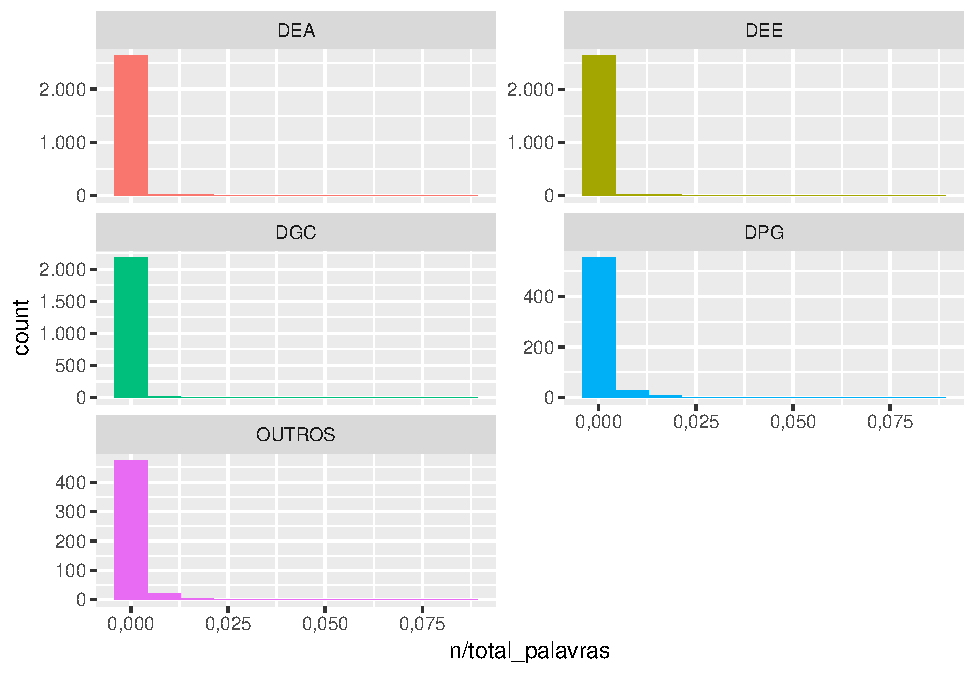
\includegraphics{markdown_v21_files/figure-latex/unnamed-chunk-22-1.pdf}

\begin{itemize}
\tightlist
\item
  Palavras mais frequentes por diretoria
\end{itemize}

\begin{Shaded}
\begin{Highlighting}[]
\NormalTok{PROP_PALAVRA =}\StringTok{ }\NormalTok{diretoria_palavras }\OperatorTok
\StringTok{    }\KeywordTok{mutate}\NormalTok{(}\DataTypeTok{palavra =} \KeywordTok{str_extract}\NormalTok{(palavra, }\StringTok{"[a-z']+"}\NormalTok{)) }\OperatorTok
\StringTok{    }\KeywordTok{count}\NormalTok{(DIRETORIA, palavra) }\OperatorTok
\StringTok{    }\KeywordTok{group_by}\NormalTok{(DIRETORIA) }\OperatorTok
\StringTok{    }\KeywordTok{mutate}\NormalTok{(}\DataTypeTok{proportion =}\NormalTok{ n }\OperatorTok{/}\StringTok{ }\KeywordTok{sum}\NormalTok{(n)) }\OperatorTok
\StringTok{    }\KeywordTok{select}\NormalTok{(}\OperatorTok{-}\NormalTok{n) }\OperatorTok
\StringTok{    }\KeywordTok{spread}\NormalTok{(DIRETORIA, proportion)}
\end{Highlighting}
\end{Shaded}

\paragraph{Gráficos de comparação de frequência de palavras por
diretorias (2 a
2)}\label{graficos-de-comparacao-de-frequencia-de-palavras-por-diretorias-2-a-2}

\texttt{COM\ STOPWORDS}

É importante ressaltar que os gráficos a seguir mostram, apenas, a
comparação de frequência de palavras existentes em ambas diretorias. Ou
seja, palavras existentes em apenas uma diretoria serão desconsideradas
para a geração destes.

\begin{itemize}
\tightlist
\item
  DEE X DEA
\end{itemize}

\begin{Shaded}
\begin{Highlighting}[]
\NormalTok{freq00 <-}\StringTok{ }\NormalTok{PROP_PALAVRA }\OperatorTok
\StringTok{    }\KeywordTok{gather}\NormalTok{(DIRETORIA, proportion, }\KeywordTok{c}\NormalTok{(}\StringTok{`}\DataTypeTok{DEA}\StringTok{`}\NormalTok{))}
  
  \KeywordTok{library}\NormalTok{(scales)}
  \CommentTok{# expect a warning about rows with missing values being removed}
  \KeywordTok{ggplot}\NormalTok{(freq00, }\KeywordTok{aes}\NormalTok{(}\DataTypeTok{x =}\NormalTok{ proportion, }\DataTypeTok{y =} \StringTok{`}\DataTypeTok{DEE}\StringTok{`}\NormalTok{,}
                        \DataTypeTok{color =} \KeywordTok{abs}\NormalTok{(}\StringTok{`}\DataTypeTok{DEE}\StringTok{`} \OperatorTok{-}\StringTok{ }\NormalTok{proportion))) }\OperatorTok{+}
\StringTok{    }\KeywordTok{geom_abline}\NormalTok{(}\DataTypeTok{color =} \StringTok{"gray40"}\NormalTok{, }\DataTypeTok{lty =} \DecValTok{2}\NormalTok{) }\OperatorTok{+}
\StringTok{    }\KeywordTok{geom_jitter}\NormalTok{(}\DataTypeTok{alpha =} \FloatTok{0.1}\NormalTok{, }\DataTypeTok{size =} \FloatTok{2.5}\NormalTok{, }\DataTypeTok{width =} \FloatTok{0.3}\NormalTok{, }\DataTypeTok{height =} \FloatTok{0.3}\NormalTok{) }\OperatorTok{+}
\StringTok{    }\KeywordTok{geom_text}\NormalTok{(}\KeywordTok{aes}\NormalTok{(}\DataTypeTok{label =}\NormalTok{ palavra), }\DataTypeTok{check_overlap =} \OtherTok{TRUE}\NormalTok{, }\DataTypeTok{vjust =} \FloatTok{1.5}\NormalTok{) }\OperatorTok{+}
\StringTok{    }\KeywordTok{scale_x_log10}\NormalTok{(}\DataTypeTok{labels =} \KeywordTok{percent_format}\NormalTok{(}\DataTypeTok{big.mark =} \StringTok{"."}\NormalTok{, }\DataTypeTok{decimal.mark =} \StringTok{","}\NormalTok{)) }\OperatorTok{+}
\StringTok{    }\KeywordTok{scale_y_log10}\NormalTok{(}\DataTypeTok{labels =} \KeywordTok{percent_format}\NormalTok{(}\DataTypeTok{big.mark =} \StringTok{"."}\NormalTok{, }\DataTypeTok{decimal.mark =} \StringTok{","}\NormalTok{)) }\OperatorTok{+}
\StringTok{    }\KeywordTok{scale_color_gradient}\NormalTok{(}\DataTypeTok{limits =} \KeywordTok{c}\NormalTok{(}\DecValTok{0}\NormalTok{, }\FloatTok{0.001}\NormalTok{),}
                         \DataTypeTok{low =} \StringTok{"darkslategray4"}\NormalTok{, }\DataTypeTok{high =} \StringTok{"gray75"}\NormalTok{) }\OperatorTok{+}
\StringTok{    }\KeywordTok{facet_wrap}\NormalTok{(}\OperatorTok{~}\NormalTok{DIRETORIA, }\DataTypeTok{ncol =} \DecValTok{1}\NormalTok{) }\OperatorTok{+}
\StringTok{    }\KeywordTok{theme}\NormalTok{(}\DataTypeTok{legend.position=}\StringTok{"none"}\NormalTok{) }\OperatorTok{+}
\StringTok{    }\KeywordTok{labs}\NormalTok{(}\DataTypeTok{y =} \StringTok{"DEE"}\NormalTok{, }\DataTypeTok{x =} \OtherTok{NULL}\NormalTok{)}
\end{Highlighting}
\end{Shaded}

\begin{verbatim}
## Warning: Removed 3487 rows containing missing values (geom_point).
\end{verbatim}

\begin{verbatim}
## Warning: Removed 3488 rows containing missing values (geom_text).
\end{verbatim}

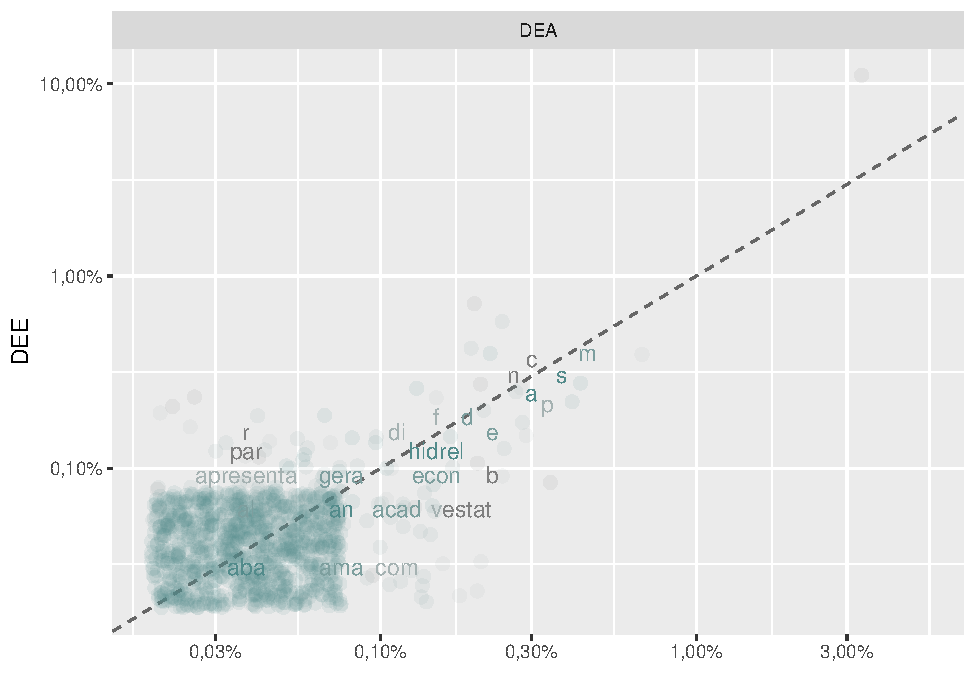
\includegraphics{markdown_v21_files/figure-latex/unnamed-chunk-25-1.pdf}

\begin{itemize}
\tightlist
\item
  DEE X DPG
\end{itemize}

\begin{Shaded}
\begin{Highlighting}[]
\NormalTok{freq01 <-}\StringTok{ }\NormalTok{PROP_PALAVRA }\OperatorTok
\StringTok{    }\KeywordTok{gather}\NormalTok{(DIRETORIA, proportion, }\KeywordTok{c}\NormalTok{(}\StringTok{`}\DataTypeTok{DPG}\StringTok{`}\NormalTok{))}
  
  \KeywordTok{library}\NormalTok{(scales)}
  \CommentTok{# expect a warning about rows with missing values being removed}
  \KeywordTok{ggplot}\NormalTok{(freq01, }\KeywordTok{aes}\NormalTok{(}\DataTypeTok{x =}\NormalTok{ proportion, }\DataTypeTok{y =} \StringTok{`}\DataTypeTok{DEE}\StringTok{`}\NormalTok{,}
                        \DataTypeTok{color =} \KeywordTok{abs}\NormalTok{(}\StringTok{`}\DataTypeTok{DEE}\StringTok{`} \OperatorTok{-}\StringTok{ }\NormalTok{proportion))) }\OperatorTok{+}
\StringTok{    }\KeywordTok{geom_abline}\NormalTok{(}\DataTypeTok{color =} \StringTok{"gray40"}\NormalTok{, }\DataTypeTok{lty =} \DecValTok{2}\NormalTok{) }\OperatorTok{+}
\StringTok{    }\KeywordTok{geom_jitter}\NormalTok{(}\DataTypeTok{alpha =} \FloatTok{0.1}\NormalTok{, }\DataTypeTok{size =} \FloatTok{2.5}\NormalTok{, }\DataTypeTok{width =} \FloatTok{0.3}\NormalTok{, }\DataTypeTok{height =} \FloatTok{0.3}\NormalTok{) }\OperatorTok{+}
\StringTok{    }\KeywordTok{geom_text}\NormalTok{(}\KeywordTok{aes}\NormalTok{(}\DataTypeTok{label =}\NormalTok{ palavra), }\DataTypeTok{check_overlap =} \OtherTok{TRUE}\NormalTok{, }\DataTypeTok{vjust =} \FloatTok{1.5}\NormalTok{) }\OperatorTok{+}
\StringTok{    }\KeywordTok{scale_x_log10}\NormalTok{(}\DataTypeTok{labels =} \KeywordTok{percent_format}\NormalTok{(}\DataTypeTok{big.mark =} \StringTok{"."}\NormalTok{, }\DataTypeTok{decimal.mark =} \StringTok{","}\NormalTok{)) }\OperatorTok{+}
\StringTok{    }\KeywordTok{scale_y_log10}\NormalTok{(}\DataTypeTok{labels =} \KeywordTok{percent_format}\NormalTok{(}\DataTypeTok{big.mark =} \StringTok{"."}\NormalTok{, }\DataTypeTok{decimal.mark =} \StringTok{","}\NormalTok{)) }\OperatorTok{+}
\StringTok{    }\KeywordTok{scale_color_gradient}\NormalTok{(}\DataTypeTok{limits =} \KeywordTok{c}\NormalTok{(}\DecValTok{0}\NormalTok{, }\FloatTok{0.001}\NormalTok{),}
                         \DataTypeTok{low =} \StringTok{"darkslategray4"}\NormalTok{, }\DataTypeTok{high =} \StringTok{"gray75"}\NormalTok{) }\OperatorTok{+}
\StringTok{    }\KeywordTok{facet_wrap}\NormalTok{(}\OperatorTok{~}\NormalTok{DIRETORIA, }\DataTypeTok{ncol =} \DecValTok{1}\NormalTok{) }\OperatorTok{+}
\StringTok{    }\KeywordTok{theme}\NormalTok{(}\DataTypeTok{legend.position=}\StringTok{"none"}\NormalTok{) }\OperatorTok{+}
\StringTok{    }\KeywordTok{labs}\NormalTok{(}\DataTypeTok{y =} \StringTok{"DEE"}\NormalTok{, }\DataTypeTok{x =} \OtherTok{NULL}\NormalTok{)}
\end{Highlighting}
\end{Shaded}

\begin{verbatim}
## Warning: Removed 4235 rows containing missing values (geom_point).
\end{verbatim}

\begin{verbatim}
## Warning: Removed 4236 rows containing missing values (geom_text).
\end{verbatim}

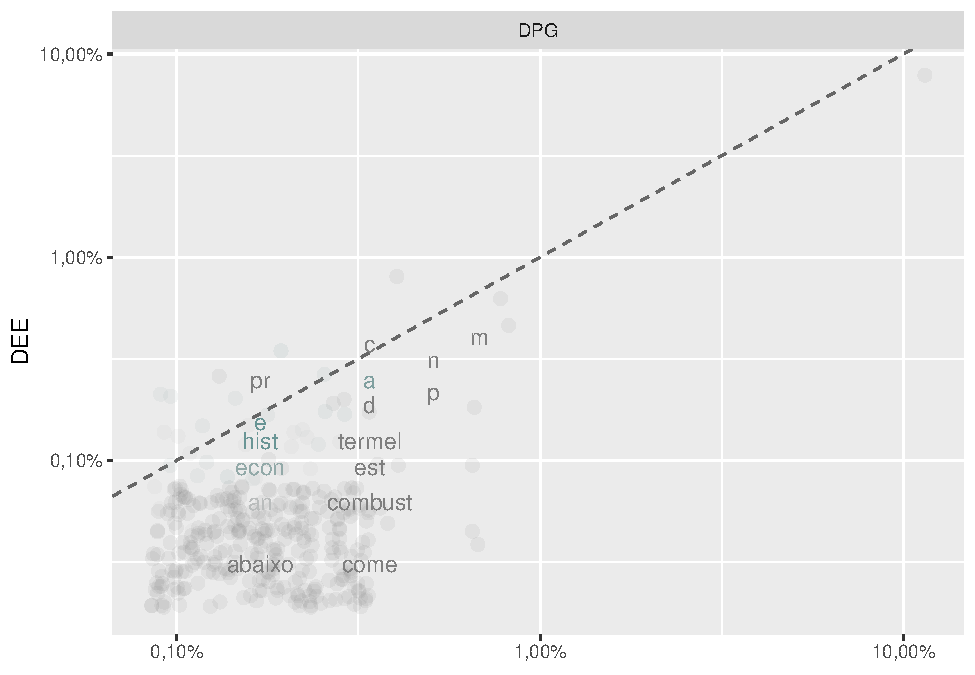
\includegraphics{markdown_v21_files/figure-latex/unnamed-chunk-26-1.pdf}

\begin{Shaded}
\begin{Highlighting}[]
\FunctionTok{Warning messages:}
\FunctionTok{1:}\AttributeTok{ Removed 4235 rows containing missing values (geom_point). }
\FunctionTok{2:}\AttributeTok{ Removed 4236 rows containing missing values (geom_text). }
\end{Highlighting}
\end{Shaded}

\begin{itemize}
\tightlist
\item
  DEE X DGC
\end{itemize}

\begin{Shaded}
\begin{Highlighting}[]
\NormalTok{freq02 <-}\StringTok{ }\NormalTok{PROP_PALAVRA }\OperatorTok
\StringTok{    }\KeywordTok{gather}\NormalTok{(DIRETORIA, proportion, }\KeywordTok{c}\NormalTok{(}\StringTok{`}\DataTypeTok{DGC}\StringTok{`}\NormalTok{))}
  
  \KeywordTok{library}\NormalTok{(scales)}
  \CommentTok{# expect a warning about rows with missing values being removed}
  \KeywordTok{ggplot}\NormalTok{(freq02, }\KeywordTok{aes}\NormalTok{(}\DataTypeTok{x =}\NormalTok{ proportion, }\DataTypeTok{y =} \StringTok{`}\DataTypeTok{DEE}\StringTok{`}\NormalTok{,}
                        \DataTypeTok{color =} \KeywordTok{abs}\NormalTok{(}\StringTok{`}\DataTypeTok{DEE}\StringTok{`} \OperatorTok{-}\StringTok{ }\NormalTok{proportion))) }\OperatorTok{+}
\StringTok{    }\KeywordTok{geom_abline}\NormalTok{(}\DataTypeTok{color =} \StringTok{"gray40"}\NormalTok{, }\DataTypeTok{lty =} \DecValTok{2}\NormalTok{) }\OperatorTok{+}
\StringTok{    }\KeywordTok{geom_jitter}\NormalTok{(}\DataTypeTok{alpha =} \FloatTok{0.1}\NormalTok{, }\DataTypeTok{size =} \FloatTok{2.5}\NormalTok{, }\DataTypeTok{width =} \FloatTok{0.3}\NormalTok{, }\DataTypeTok{height =} \FloatTok{0.3}\NormalTok{) }\OperatorTok{+}
\StringTok{    }\KeywordTok{geom_text}\NormalTok{(}\KeywordTok{aes}\NormalTok{(}\DataTypeTok{label =}\NormalTok{ palavra), }\DataTypeTok{check_overlap =} \OtherTok{TRUE}\NormalTok{, }\DataTypeTok{vjust =} \FloatTok{1.5}\NormalTok{) }\OperatorTok{+}
\StringTok{    }\KeywordTok{scale_x_log10}\NormalTok{(}\DataTypeTok{labels =} \KeywordTok{percent_format}\NormalTok{(}\DataTypeTok{big.mark =} \StringTok{"."}\NormalTok{, }\DataTypeTok{decimal.mark =} \StringTok{","}\NormalTok{)) }\OperatorTok{+}
\StringTok{    }\KeywordTok{scale_y_log10}\NormalTok{(}\DataTypeTok{labels =} \KeywordTok{percent_format}\NormalTok{(}\DataTypeTok{big.mark =} \StringTok{"."}\NormalTok{, }\DataTypeTok{decimal.mark =} \StringTok{","}\NormalTok{)) }\OperatorTok{+}
\StringTok{    }\KeywordTok{scale_color_gradient}\NormalTok{(}\DataTypeTok{limits =} \KeywordTok{c}\NormalTok{(}\DecValTok{0}\NormalTok{, }\FloatTok{0.001}\NormalTok{),}
                         \DataTypeTok{low =} \StringTok{"darkslategray4"}\NormalTok{, }\DataTypeTok{high =} \StringTok{"gray75"}\NormalTok{) }\OperatorTok{+}
\StringTok{    }\KeywordTok{facet_wrap}\NormalTok{(}\OperatorTok{~}\NormalTok{DIRETORIA, }\DataTypeTok{ncol =} \DecValTok{1}\NormalTok{) }\OperatorTok{+}
\StringTok{    }\KeywordTok{theme}\NormalTok{(}\DataTypeTok{legend.position=}\StringTok{"none"}\NormalTok{) }\OperatorTok{+}
\StringTok{    }\KeywordTok{labs}\NormalTok{(}\DataTypeTok{y =} \StringTok{"DEE"}\NormalTok{, }\DataTypeTok{x =} \OtherTok{NULL}\NormalTok{)}
\end{Highlighting}
\end{Shaded}

\begin{verbatim}
## Warning: Removed 3794 rows containing missing values (geom_point).
\end{verbatim}

\begin{verbatim}
## Warning: Removed 3795 rows containing missing values (geom_text).
\end{verbatim}

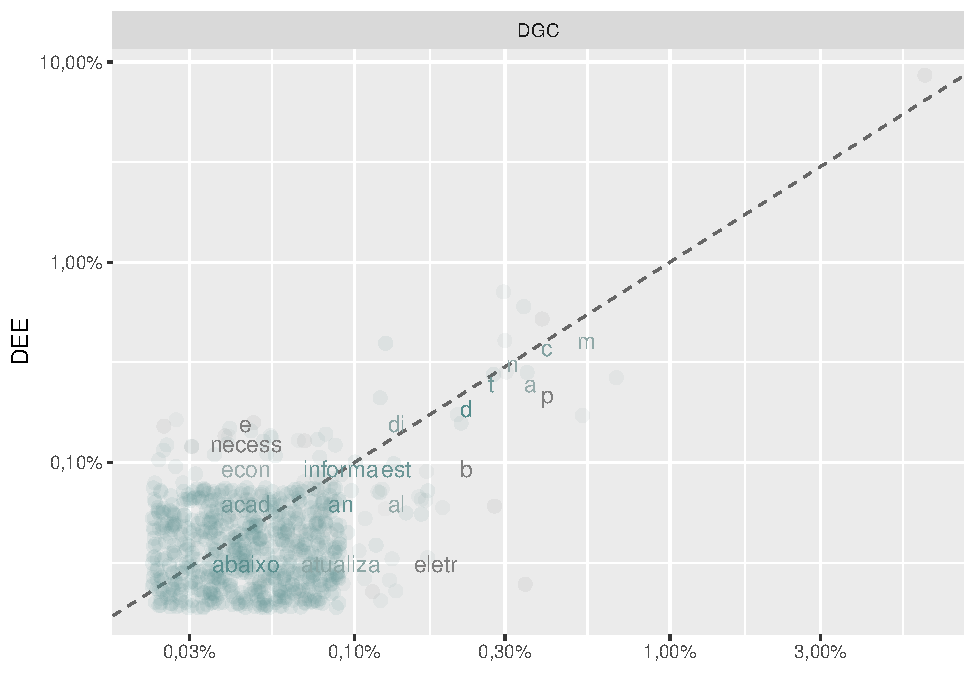
\includegraphics{markdown_v21_files/figure-latex/unnamed-chunk-27-1.pdf}

\begin{Shaded}
\begin{Highlighting}[]
\FunctionTok{Warning messages:}
\FunctionTok{1:}\AttributeTok{ Removed 3794 rows containing missing values (geom_point). }
\FunctionTok{2:}\AttributeTok{ Removed 3795 rows containing missing values (geom_text).}
\end{Highlighting}
\end{Shaded}

\begin{itemize}
\tightlist
\item
  DEE X OUTROS
\end{itemize}

\begin{Shaded}
\begin{Highlighting}[]
\NormalTok{freq03 <-}\StringTok{ }\NormalTok{PROP_PALAVRA }\OperatorTok
\StringTok{    }\KeywordTok{gather}\NormalTok{(DIRETORIA, proportion, }\KeywordTok{c}\NormalTok{(}\StringTok{`}\DataTypeTok{OUTROS}\StringTok{`}\NormalTok{))}
  
  \KeywordTok{library}\NormalTok{(scales)}
  \CommentTok{# expect a warning about rows with missing values being removed}
  \KeywordTok{ggplot}\NormalTok{(freq03, }\KeywordTok{aes}\NormalTok{(}\DataTypeTok{x =}\NormalTok{ proportion, }\DataTypeTok{y =} \StringTok{`}\DataTypeTok{DEE}\StringTok{`}\NormalTok{,}
                        \DataTypeTok{color =} \KeywordTok{abs}\NormalTok{(}\StringTok{`}\DataTypeTok{DEE}\StringTok{`} \OperatorTok{-}\StringTok{ }\NormalTok{proportion))) }\OperatorTok{+}
\StringTok{    }\KeywordTok{geom_abline}\NormalTok{(}\DataTypeTok{color =} \StringTok{"gray40"}\NormalTok{, }\DataTypeTok{lty =} \DecValTok{2}\NormalTok{) }\OperatorTok{+}
\StringTok{    }\KeywordTok{geom_jitter}\NormalTok{(}\DataTypeTok{alpha =} \FloatTok{0.1}\NormalTok{, }\DataTypeTok{size =} \FloatTok{2.5}\NormalTok{, }\DataTypeTok{width =} \FloatTok{0.3}\NormalTok{, }\DataTypeTok{height =} \FloatTok{0.3}\NormalTok{) }\OperatorTok{+}
\StringTok{    }\KeywordTok{geom_text}\NormalTok{(}\KeywordTok{aes}\NormalTok{(}\DataTypeTok{label =}\NormalTok{ palavra), }\DataTypeTok{check_overlap =} \OtherTok{TRUE}\NormalTok{, }\DataTypeTok{vjust =} \FloatTok{1.5}\NormalTok{) }\OperatorTok{+}
\StringTok{    }\KeywordTok{scale_x_log10}\NormalTok{(}\DataTypeTok{labels =} \KeywordTok{percent_format}\NormalTok{(}\DataTypeTok{big.mark =} \StringTok{"."}\NormalTok{, }\DataTypeTok{decimal.mark =} \StringTok{","}\NormalTok{)) }\OperatorTok{+}
\StringTok{    }\KeywordTok{scale_y_log10}\NormalTok{(}\DataTypeTok{labels =} \KeywordTok{percent_format}\NormalTok{(}\DataTypeTok{big.mark =} \StringTok{"."}\NormalTok{, }\DataTypeTok{decimal.mark =} \StringTok{","}\NormalTok{)) }\OperatorTok{+}
\StringTok{    }\KeywordTok{scale_color_gradient}\NormalTok{(}\DataTypeTok{limits =} \KeywordTok{c}\NormalTok{(}\DecValTok{0}\NormalTok{, }\FloatTok{0.001}\NormalTok{),}
                         \DataTypeTok{low =} \StringTok{"darkslategray4"}\NormalTok{, }\DataTypeTok{high =} \StringTok{"gray75"}\NormalTok{) }\OperatorTok{+}
\StringTok{    }\KeywordTok{facet_wrap}\NormalTok{(}\OperatorTok{~}\NormalTok{DIRETORIA, }\DataTypeTok{ncol =} \DecValTok{1}\NormalTok{) }\OperatorTok{+}
\StringTok{    }\KeywordTok{theme}\NormalTok{(}\DataTypeTok{legend.position=}\StringTok{"none"}\NormalTok{) }\OperatorTok{+}
\StringTok{    }\KeywordTok{labs}\NormalTok{(}\DataTypeTok{y =} \StringTok{"DEE"}\NormalTok{, }\DataTypeTok{x =} \OtherTok{NULL}\NormalTok{)}
\end{Highlighting}
\end{Shaded}

\begin{verbatim}
## Warning: Removed 4273 rows containing missing values (geom_point).
\end{verbatim}

\begin{verbatim}
## Warning: Removed 4274 rows containing missing values (geom_text).
\end{verbatim}

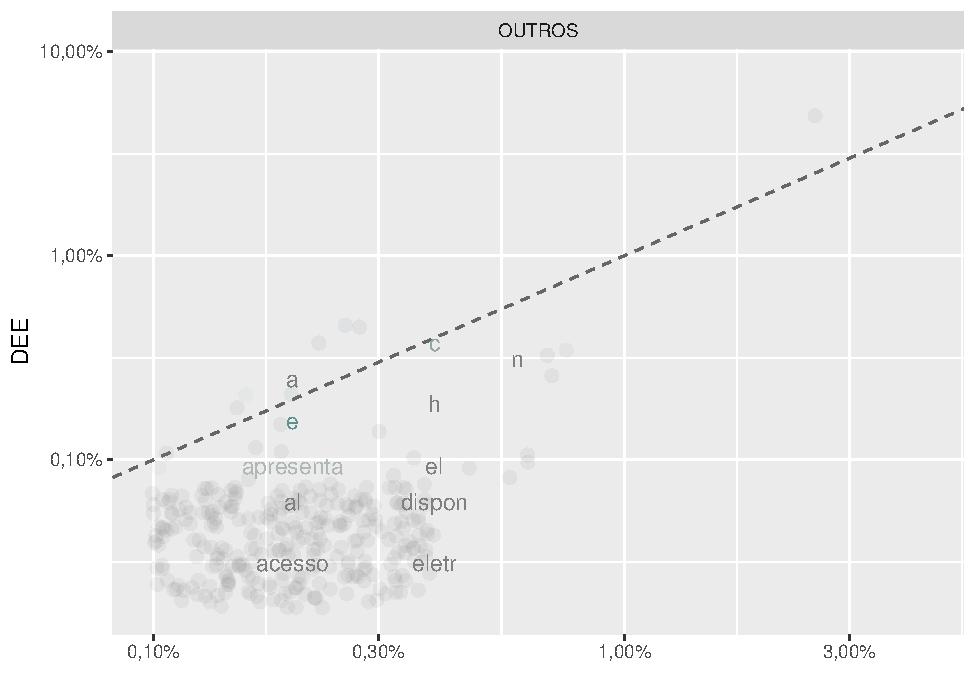
\includegraphics{markdown_v21_files/figure-latex/unnamed-chunk-28-1.pdf}

\begin{Shaded}
\begin{Highlighting}[]
\FunctionTok{Warning messages:}
\FunctionTok{1:}\AttributeTok{ Removed 4273 rows containing missing values (geom_point). }
\FunctionTok{2:}\AttributeTok{ Removed 4274 rows containing missing values (geom_text).}
\end{Highlighting}
\end{Shaded}

\begin{itemize}
\tightlist
\item
  DEA X DPG
\end{itemize}

\begin{Shaded}
\begin{Highlighting}[]
\NormalTok{freq04 <-}\StringTok{ }\NormalTok{PROP_PALAVRA }\OperatorTok
\StringTok{    }\KeywordTok{gather}\NormalTok{(DIRETORIA, proportion, }\KeywordTok{c}\NormalTok{(}\StringTok{`}\DataTypeTok{DPG}\StringTok{`}\NormalTok{))}
  
  \KeywordTok{library}\NormalTok{(scales)}
  \CommentTok{# expect a warning about rows with missing values being removed}
  \KeywordTok{ggplot}\NormalTok{(freq04, }\KeywordTok{aes}\NormalTok{(}\DataTypeTok{x =}\NormalTok{ proportion, }\DataTypeTok{y =} \StringTok{`}\DataTypeTok{DEA}\StringTok{`}\NormalTok{,}
                        \DataTypeTok{color =} \KeywordTok{abs}\NormalTok{(}\StringTok{`}\DataTypeTok{DEA}\StringTok{`} \OperatorTok{-}\StringTok{ }\NormalTok{proportion))) }\OperatorTok{+}
\StringTok{    }\KeywordTok{geom_abline}\NormalTok{(}\DataTypeTok{color =} \StringTok{"gray40"}\NormalTok{, }\DataTypeTok{lty =} \DecValTok{2}\NormalTok{) }\OperatorTok{+}
\StringTok{    }\KeywordTok{geom_jitter}\NormalTok{(}\DataTypeTok{alpha =} \FloatTok{0.1}\NormalTok{, }\DataTypeTok{size =} \FloatTok{2.5}\NormalTok{, }\DataTypeTok{width =} \FloatTok{0.3}\NormalTok{, }\DataTypeTok{height =} \FloatTok{0.3}\NormalTok{) }\OperatorTok{+}
\StringTok{    }\KeywordTok{geom_text}\NormalTok{(}\KeywordTok{aes}\NormalTok{(}\DataTypeTok{label =}\NormalTok{ palavra), }\DataTypeTok{check_overlap =} \OtherTok{TRUE}\NormalTok{, }\DataTypeTok{vjust =} \FloatTok{1.5}\NormalTok{) }\OperatorTok{+}
\StringTok{    }\KeywordTok{scale_x_log10}\NormalTok{(}\DataTypeTok{labels =} \KeywordTok{percent_format}\NormalTok{(}\DataTypeTok{big.mark =} \StringTok{"."}\NormalTok{, }\DataTypeTok{decimal.mark =} \StringTok{","}\NormalTok{)) }\OperatorTok{+}
\StringTok{    }\KeywordTok{scale_y_log10}\NormalTok{(}\DataTypeTok{labels =} \KeywordTok{percent_format}\NormalTok{(}\DataTypeTok{big.mark =} \StringTok{"."}\NormalTok{, }\DataTypeTok{decimal.mark =} \StringTok{","}\NormalTok{)) }\OperatorTok{+}
\StringTok{    }\KeywordTok{scale_color_gradient}\NormalTok{(}\DataTypeTok{limits =} \KeywordTok{c}\NormalTok{(}\DecValTok{0}\NormalTok{, }\FloatTok{0.001}\NormalTok{),}
                         \DataTypeTok{low =} \StringTok{"darkslategray4"}\NormalTok{, }\DataTypeTok{high =} \StringTok{"gray75"}\NormalTok{) }\OperatorTok{+}
\StringTok{    }\KeywordTok{facet_wrap}\NormalTok{(}\OperatorTok{~}\NormalTok{DIRETORIA, }\DataTypeTok{ncol =} \DecValTok{1}\NormalTok{) }\OperatorTok{+}
\StringTok{    }\KeywordTok{theme}\NormalTok{(}\DataTypeTok{legend.position=}\StringTok{"none"}\NormalTok{) }\OperatorTok{+}
\StringTok{    }\KeywordTok{labs}\NormalTok{(}\DataTypeTok{y =} \StringTok{"DEA"}\NormalTok{, }\DataTypeTok{x =} \OtherTok{NULL}\NormalTok{)}
\end{Highlighting}
\end{Shaded}

\begin{verbatim}
## Warning: Removed 4221 rows containing missing values (geom_point).
\end{verbatim}

\begin{verbatim}
## Warning: Removed 4222 rows containing missing values (geom_text).
\end{verbatim}

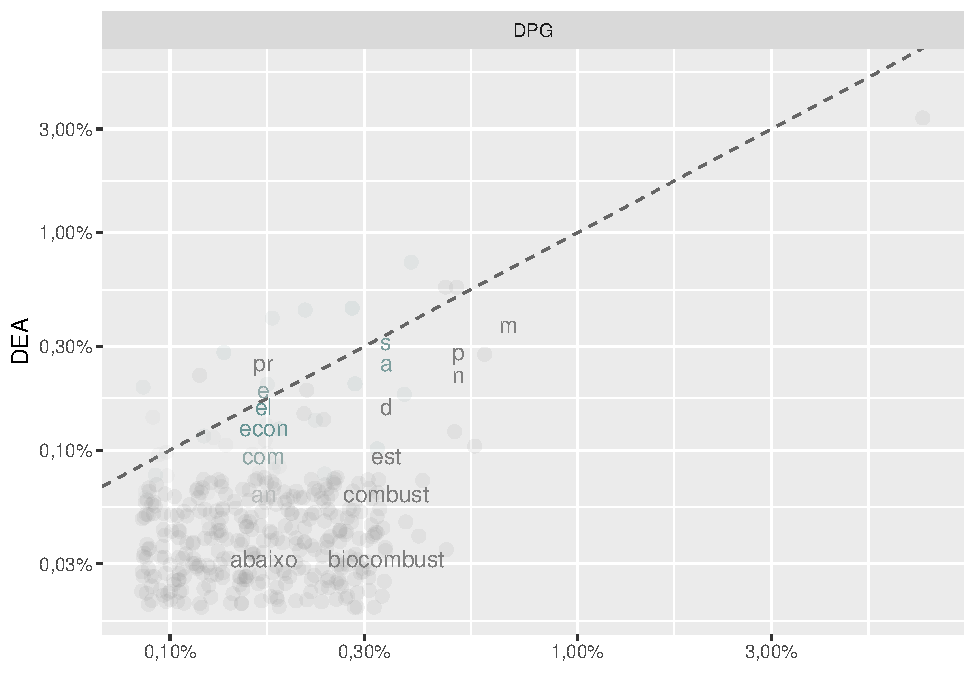
\includegraphics{markdown_v21_files/figure-latex/unnamed-chunk-29-1.pdf}

\begin{Shaded}
\begin{Highlighting}[]
\FunctionTok{Warning messages:}
\FunctionTok{1:}\AttributeTok{ Removed 4221 rows containing missing values (geom_point). }
\FunctionTok{2:}\AttributeTok{ Removed 4222 rows containing missing values (geom_text).}
\end{Highlighting}
\end{Shaded}

\begin{itemize}
\tightlist
\item
  DEA X DGC
\end{itemize}

\begin{Shaded}
\begin{Highlighting}[]
\NormalTok{freq05 <-}\StringTok{ }\NormalTok{PROP_PALAVRA }\OperatorTok
\StringTok{    }\KeywordTok{gather}\NormalTok{(DIRETORIA, proportion, }\KeywordTok{c}\NormalTok{(}\StringTok{`}\DataTypeTok{DGC}\StringTok{`}\NormalTok{))}
  
  \KeywordTok{library}\NormalTok{(scales)}
  \CommentTok{# expect a warning about rows with missing values being removed}
  \KeywordTok{ggplot}\NormalTok{(freq05, }\KeywordTok{aes}\NormalTok{(}\DataTypeTok{x =}\NormalTok{ proportion, }\DataTypeTok{y =} \StringTok{`}\DataTypeTok{DEA}\StringTok{`}\NormalTok{,}
                        \DataTypeTok{color =} \KeywordTok{abs}\NormalTok{(}\StringTok{`}\DataTypeTok{DEA}\StringTok{`} \OperatorTok{-}\StringTok{ }\NormalTok{proportion))) }\OperatorTok{+}
\StringTok{    }\KeywordTok{geom_abline}\NormalTok{(}\DataTypeTok{color =} \StringTok{"gray40"}\NormalTok{, }\DataTypeTok{lty =} \DecValTok{2}\NormalTok{) }\OperatorTok{+}
\StringTok{    }\KeywordTok{geom_jitter}\NormalTok{(}\DataTypeTok{alpha =} \FloatTok{0.1}\NormalTok{, }\DataTypeTok{size =} \FloatTok{2.5}\NormalTok{, }\DataTypeTok{width =} \FloatTok{0.3}\NormalTok{, }\DataTypeTok{height =} \FloatTok{0.3}\NormalTok{) }\OperatorTok{+}
\StringTok{    }\KeywordTok{geom_text}\NormalTok{(}\KeywordTok{aes}\NormalTok{(}\DataTypeTok{label =}\NormalTok{ palavra), }\DataTypeTok{check_overlap =} \OtherTok{TRUE}\NormalTok{, }\DataTypeTok{vjust =} \FloatTok{1.5}\NormalTok{) }\OperatorTok{+}
\StringTok{    }\KeywordTok{scale_x_log10}\NormalTok{(}\DataTypeTok{labels =} \KeywordTok{percent_format}\NormalTok{(}\DataTypeTok{big.mark =} \StringTok{"."}\NormalTok{, }\DataTypeTok{decimal.mark =} \StringTok{","}\NormalTok{)) }\OperatorTok{+}
\StringTok{    }\KeywordTok{scale_y_log10}\NormalTok{(}\DataTypeTok{labels =} \KeywordTok{percent_format}\NormalTok{(}\DataTypeTok{big.mark =} \StringTok{"."}\NormalTok{, }\DataTypeTok{decimal.mark =} \StringTok{","}\NormalTok{)) }\OperatorTok{+}
\StringTok{    }\KeywordTok{scale_color_gradient}\NormalTok{(}\DataTypeTok{limits =} \KeywordTok{c}\NormalTok{(}\DecValTok{0}\NormalTok{, }\FloatTok{0.001}\NormalTok{),}
                         \DataTypeTok{low =} \StringTok{"darkslategray4"}\NormalTok{, }\DataTypeTok{high =} \StringTok{"gray75"}\NormalTok{) }\OperatorTok{+}
\StringTok{    }\KeywordTok{facet_wrap}\NormalTok{(}\OperatorTok{~}\NormalTok{DIRETORIA, }\DataTypeTok{ncol =} \DecValTok{1}\NormalTok{) }\OperatorTok{+}
\StringTok{    }\KeywordTok{theme}\NormalTok{(}\DataTypeTok{legend.position=}\StringTok{"none"}\NormalTok{) }\OperatorTok{+}
\StringTok{    }\KeywordTok{labs}\NormalTok{(}\DataTypeTok{y =} \StringTok{"DEA"}\NormalTok{, }\DataTypeTok{x =} \OtherTok{NULL}\NormalTok{)}
\end{Highlighting}
\end{Shaded}

\begin{verbatim}
## Warning: Removed 3812 rows containing missing values (geom_point).
\end{verbatim}

\begin{verbatim}
## Warning: Removed 3813 rows containing missing values (geom_text).
\end{verbatim}

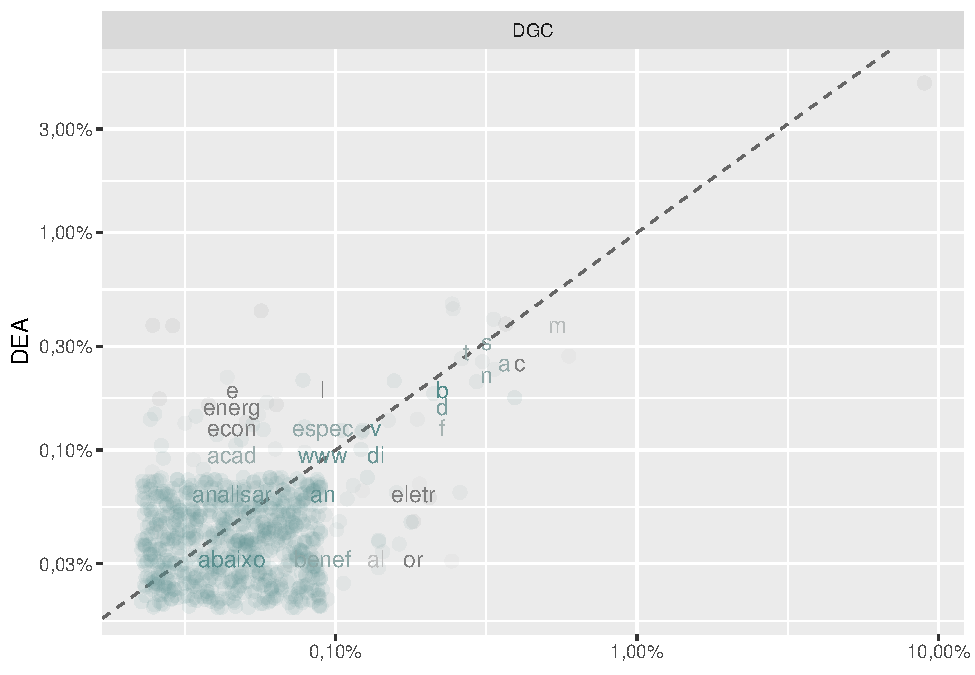
\includegraphics{markdown_v21_files/figure-latex/unnamed-chunk-30-1.pdf}

\begin{Shaded}
\begin{Highlighting}[]
\FunctionTok{Warning messages:}
\FunctionTok{1:}\AttributeTok{ Removed 3812 rows containing missing values (geom_point). }
\FunctionTok{2:}\AttributeTok{ Removed 3813 rows containing missing values (geom_text).}
\end{Highlighting}
\end{Shaded}

\begin{itemize}
\tightlist
\item
  DEA X OUTROS
\end{itemize}

\begin{Shaded}
\begin{Highlighting}[]
\NormalTok{freq06 <-}\StringTok{ }\NormalTok{PROP_PALAVRA }\OperatorTok
\StringTok{    }\KeywordTok{gather}\NormalTok{(DIRETORIA, proportion, }\KeywordTok{c}\NormalTok{(}\StringTok{`}\DataTypeTok{OUTROS}\StringTok{`}\NormalTok{))}
  
  \KeywordTok{library}\NormalTok{(scales)}
  \CommentTok{# expect a warning about rows with missing values being removed}
  \KeywordTok{ggplot}\NormalTok{(freq06, }\KeywordTok{aes}\NormalTok{(}\DataTypeTok{x =}\NormalTok{ proportion, }\DataTypeTok{y =} \StringTok{`}\DataTypeTok{DEA}\StringTok{`}\NormalTok{,}
                        \DataTypeTok{color =} \KeywordTok{abs}\NormalTok{(}\StringTok{`}\DataTypeTok{DEA}\StringTok{`} \OperatorTok{-}\StringTok{ }\NormalTok{proportion))) }\OperatorTok{+}
\StringTok{    }\KeywordTok{geom_abline}\NormalTok{(}\DataTypeTok{color =} \StringTok{"gray40"}\NormalTok{, }\DataTypeTok{lty =} \DecValTok{2}\NormalTok{) }\OperatorTok{+}
\StringTok{    }\KeywordTok{geom_jitter}\NormalTok{(}\DataTypeTok{alpha =} \FloatTok{0.1}\NormalTok{, }\DataTypeTok{size =} \FloatTok{2.5}\NormalTok{, }\DataTypeTok{width =} \FloatTok{0.3}\NormalTok{, }\DataTypeTok{height =} \FloatTok{0.3}\NormalTok{) }\OperatorTok{+}
\StringTok{    }\KeywordTok{geom_text}\NormalTok{(}\KeywordTok{aes}\NormalTok{(}\DataTypeTok{label =}\NormalTok{ palavra), }\DataTypeTok{check_overlap =} \OtherTok{TRUE}\NormalTok{, }\DataTypeTok{vjust =} \FloatTok{1.5}\NormalTok{) }\OperatorTok{+}
\StringTok{    }\KeywordTok{scale_x_log10}\NormalTok{(}\DataTypeTok{labels =} \KeywordTok{percent_format}\NormalTok{(}\DataTypeTok{big.mark =} \StringTok{"."}\NormalTok{, }\DataTypeTok{decimal.mark =} \StringTok{","}\NormalTok{)) }\OperatorTok{+}
\StringTok{    }\KeywordTok{scale_y_log10}\NormalTok{(}\DataTypeTok{labels =} \KeywordTok{percent_format}\NormalTok{(}\DataTypeTok{big.mark =} \StringTok{"."}\NormalTok{, }\DataTypeTok{decimal.mark =} \StringTok{","}\NormalTok{)) }\OperatorTok{+}
\StringTok{    }\KeywordTok{scale_color_gradient}\NormalTok{(}\DataTypeTok{limits =} \KeywordTok{c}\NormalTok{(}\DecValTok{0}\NormalTok{, }\FloatTok{0.001}\NormalTok{),}
                         \DataTypeTok{low =} \StringTok{"darkslategray4"}\NormalTok{, }\DataTypeTok{high =} \StringTok{"gray75"}\NormalTok{) }\OperatorTok{+}
\StringTok{    }\KeywordTok{facet_wrap}\NormalTok{(}\OperatorTok{~}\NormalTok{DIRETORIA, }\DataTypeTok{ncol =} \DecValTok{1}\NormalTok{) }\OperatorTok{+}
\StringTok{    }\KeywordTok{theme}\NormalTok{(}\DataTypeTok{legend.position=}\StringTok{"none"}\NormalTok{) }\OperatorTok{+}
\StringTok{    }\KeywordTok{labs}\NormalTok{(}\DataTypeTok{y =} \StringTok{"DEA"}\NormalTok{, }\DataTypeTok{x =} \OtherTok{NULL}\NormalTok{)}
\end{Highlighting}
\end{Shaded}

\begin{verbatim}
## Warning: Removed 4303 rows containing missing values (geom_point).
\end{verbatim}

\begin{verbatim}
## Warning: Removed 4304 rows containing missing values (geom_text).
\end{verbatim}

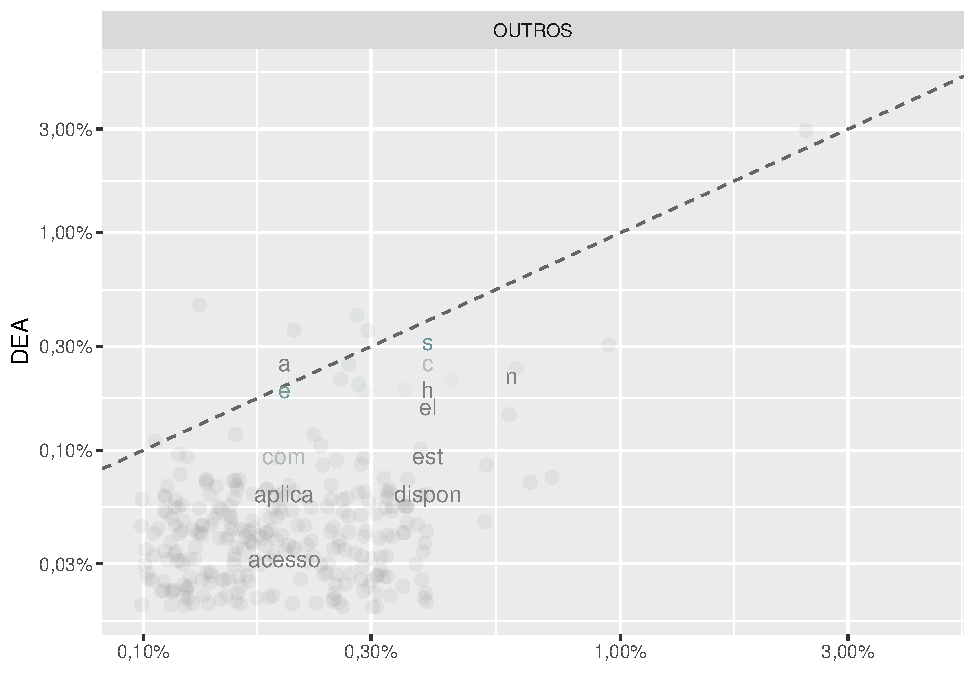
\includegraphics{markdown_v21_files/figure-latex/unnamed-chunk-31-1.pdf}

\begin{Shaded}
\begin{Highlighting}[]
\FunctionTok{Warning messages:}
\FunctionTok{1:}\AttributeTok{ Removed 4303 rows containing missing values (geom_point). }
\FunctionTok{2:}\AttributeTok{ Removed 4304 rows containing missing values (geom_text). }
\end{Highlighting}
\end{Shaded}

\begin{itemize}
\tightlist
\item
  DPG X DGC
\end{itemize}

\begin{Shaded}
\begin{Highlighting}[]
\NormalTok{freq07 <-}\StringTok{ }\NormalTok{PROP_PALAVRA }\OperatorTok
\StringTok{    }\KeywordTok{gather}\NormalTok{(DIRETORIA, proportion, }\KeywordTok{c}\NormalTok{(}\StringTok{`}\DataTypeTok{DGC}\StringTok{`}\NormalTok{))}
  
  \KeywordTok{library}\NormalTok{(scales)}
  \CommentTok{# expect a warning about rows with missing values being removed}
  \KeywordTok{ggplot}\NormalTok{(freq07, }\KeywordTok{aes}\NormalTok{(}\DataTypeTok{x =}\NormalTok{ proportion, }\DataTypeTok{y =} \StringTok{`}\DataTypeTok{DPG}\StringTok{`}\NormalTok{,}
                        \DataTypeTok{color =} \KeywordTok{abs}\NormalTok{(}\StringTok{`}\DataTypeTok{DPG}\StringTok{`} \OperatorTok{-}\StringTok{ }\NormalTok{proportion))) }\OperatorTok{+}
\StringTok{    }\KeywordTok{geom_abline}\NormalTok{(}\DataTypeTok{color =} \StringTok{"gray40"}\NormalTok{, }\DataTypeTok{lty =} \DecValTok{2}\NormalTok{) }\OperatorTok{+}
\StringTok{    }\KeywordTok{geom_jitter}\NormalTok{(}\DataTypeTok{alpha =} \FloatTok{0.1}\NormalTok{, }\DataTypeTok{size =} \FloatTok{2.5}\NormalTok{, }\DataTypeTok{width =} \FloatTok{0.3}\NormalTok{, }\DataTypeTok{height =} \FloatTok{0.3}\NormalTok{) }\OperatorTok{+}
\StringTok{    }\KeywordTok{geom_text}\NormalTok{(}\KeywordTok{aes}\NormalTok{(}\DataTypeTok{label =}\NormalTok{ palavra), }\DataTypeTok{check_overlap =} \OtherTok{TRUE}\NormalTok{, }\DataTypeTok{vjust =} \FloatTok{1.5}\NormalTok{) }\OperatorTok{+}
\StringTok{    }\KeywordTok{scale_x_log10}\NormalTok{(}\DataTypeTok{labels =} \KeywordTok{percent_format}\NormalTok{(}\DataTypeTok{big.mark =} \StringTok{"."}\NormalTok{, }\DataTypeTok{decimal.mark =} \StringTok{","}\NormalTok{)) }\OperatorTok{+}
\StringTok{    }\KeywordTok{scale_y_log10}\NormalTok{(}\DataTypeTok{labels =} \KeywordTok{percent_format}\NormalTok{(}\DataTypeTok{big.mark =} \StringTok{"."}\NormalTok{, }\DataTypeTok{decimal.mark =} \StringTok{","}\NormalTok{)) }\OperatorTok{+}
\StringTok{    }\KeywordTok{scale_color_gradient}\NormalTok{(}\DataTypeTok{limits =} \KeywordTok{c}\NormalTok{(}\DecValTok{0}\NormalTok{, }\FloatTok{0.001}\NormalTok{),}
                         \DataTypeTok{low =} \StringTok{"darkslategray4"}\NormalTok{, }\DataTypeTok{high =} \StringTok{"gray75"}\NormalTok{) }\OperatorTok{+}
\StringTok{    }\KeywordTok{facet_wrap}\NormalTok{(}\OperatorTok{~}\NormalTok{DIRETORIA, }\DataTypeTok{ncol =} \DecValTok{1}\NormalTok{) }\OperatorTok{+}
\StringTok{    }\KeywordTok{theme}\NormalTok{(}\DataTypeTok{legend.position=}\StringTok{"none"}\NormalTok{) }\OperatorTok{+}
\StringTok{    }\KeywordTok{labs}\NormalTok{(}\DataTypeTok{y =} \StringTok{"DPG"}\NormalTok{, }\DataTypeTok{x =} \OtherTok{NULL}\NormalTok{)}
\end{Highlighting}
\end{Shaded}

\begin{verbatim}
## Warning: Removed 4296 rows containing missing values (geom_point).
\end{verbatim}

\begin{verbatim}
## Warning: Removed 4297 rows containing missing values (geom_text).
\end{verbatim}

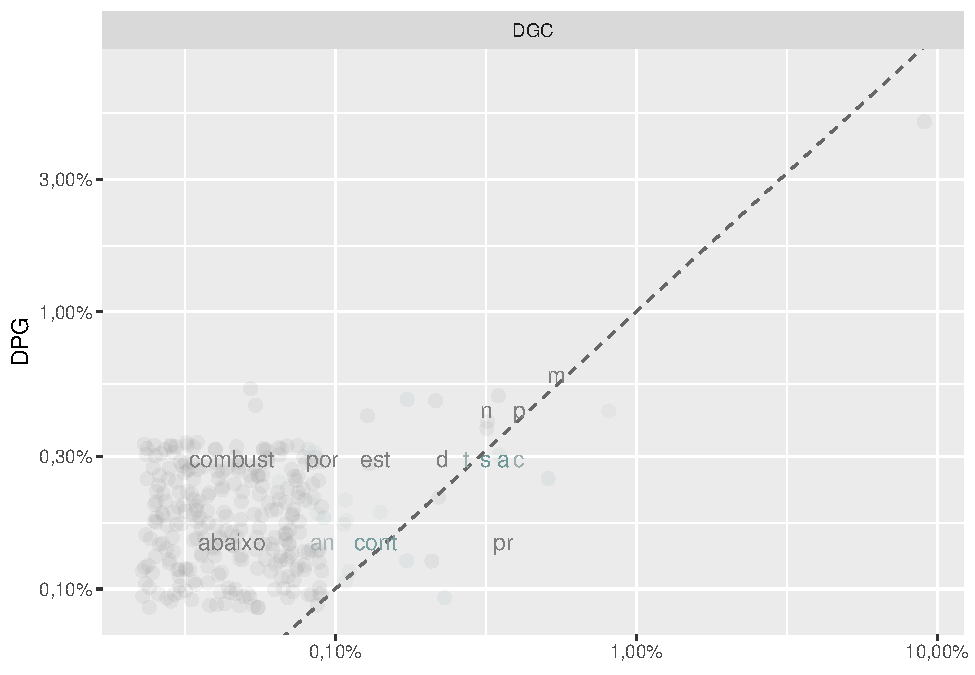
\includegraphics{markdown_v21_files/figure-latex/unnamed-chunk-32-1.pdf}

\begin{Shaded}
\begin{Highlighting}[]
\FunctionTok{Warning messages:}
\FunctionTok{1:}\AttributeTok{ Removed 4296 rows containing missing values (geom_point). }
\FunctionTok{2:}\AttributeTok{ Removed 4297 rows containing missing values (geom_text). }
\end{Highlighting}
\end{Shaded}

\begin{itemize}
\tightlist
\item
  DPG X OUTROS
\end{itemize}

\begin{Shaded}
\begin{Highlighting}[]
\NormalTok{freq08 <-}\StringTok{ }\NormalTok{PROP_PALAVRA }\OperatorTok
\StringTok{    }\KeywordTok{gather}\NormalTok{(DIRETORIA, proportion, }\KeywordTok{c}\NormalTok{(}\StringTok{`}\DataTypeTok{OUTROS}\StringTok{`}\NormalTok{))}
  
  \KeywordTok{library}\NormalTok{(scales)}
  \CommentTok{# expect a warning about rows with missing values being removed}
  \KeywordTok{ggplot}\NormalTok{(freq08, }\KeywordTok{aes}\NormalTok{(}\DataTypeTok{x =}\NormalTok{ proportion, }\DataTypeTok{y =} \StringTok{`}\DataTypeTok{DPG}\StringTok{`}\NormalTok{,}
                        \DataTypeTok{color =} \KeywordTok{abs}\NormalTok{(}\StringTok{`}\DataTypeTok{DPG}\StringTok{`} \OperatorTok{-}\StringTok{ }\NormalTok{proportion))) }\OperatorTok{+}
\StringTok{    }\KeywordTok{geom_abline}\NormalTok{(}\DataTypeTok{color =} \StringTok{"gray40"}\NormalTok{, }\DataTypeTok{lty =} \DecValTok{2}\NormalTok{) }\OperatorTok{+}
\StringTok{    }\KeywordTok{geom_jitter}\NormalTok{(}\DataTypeTok{alpha =} \FloatTok{0.1}\NormalTok{, }\DataTypeTok{size =} \FloatTok{2.5}\NormalTok{, }\DataTypeTok{width =} \FloatTok{0.3}\NormalTok{, }\DataTypeTok{height =} \FloatTok{0.3}\NormalTok{) }\OperatorTok{+}
\StringTok{    }\KeywordTok{geom_text}\NormalTok{(}\KeywordTok{aes}\NormalTok{(}\DataTypeTok{label =}\NormalTok{ palavra), }\DataTypeTok{check_overlap =} \OtherTok{TRUE}\NormalTok{, }\DataTypeTok{vjust =} \FloatTok{1.5}\NormalTok{) }\OperatorTok{+}
\StringTok{    }\KeywordTok{scale_x_log10}\NormalTok{(}\DataTypeTok{labels =} \KeywordTok{percent_format}\NormalTok{(}\DataTypeTok{big.mark =} \StringTok{"."}\NormalTok{, }\DataTypeTok{decimal.mark =} \StringTok{","}\NormalTok{)) }\OperatorTok{+}
\StringTok{    }\KeywordTok{scale_y_log10}\NormalTok{(}\DataTypeTok{labels =} \KeywordTok{percent_format}\NormalTok{(}\DataTypeTok{big.mark =} \StringTok{"."}\NormalTok{, }\DataTypeTok{decimal.mark =} \StringTok{","}\NormalTok{)) }\OperatorTok{+}
\StringTok{    }\KeywordTok{scale_color_gradient}\NormalTok{(}\DataTypeTok{limits =} \KeywordTok{c}\NormalTok{(}\DecValTok{0}\NormalTok{, }\FloatTok{0.001}\NormalTok{),}
                         \DataTypeTok{low =} \StringTok{"darkslategray4"}\NormalTok{, }\DataTypeTok{high =} \StringTok{"gray75"}\NormalTok{) }\OperatorTok{+}
\StringTok{    }\KeywordTok{facet_wrap}\NormalTok{(}\OperatorTok{~}\NormalTok{DIRETORIA, }\DataTypeTok{ncol =} \DecValTok{1}\NormalTok{) }\OperatorTok{+}
\StringTok{    }\KeywordTok{theme}\NormalTok{(}\DataTypeTok{legend.position=}\StringTok{"none"}\NormalTok{) }\OperatorTok{+}
\StringTok{    }\KeywordTok{labs}\NormalTok{(}\DataTypeTok{y =} \StringTok{"DPG"}\NormalTok{, }\DataTypeTok{x =} \OtherTok{NULL}\NormalTok{)}
\end{Highlighting}
\end{Shaded}

\begin{verbatim}
## Warning: Removed 4450 rows containing missing values (geom_point).
\end{verbatim}

\begin{verbatim}
## Warning: Removed 4451 rows containing missing values (geom_text).
\end{verbatim}

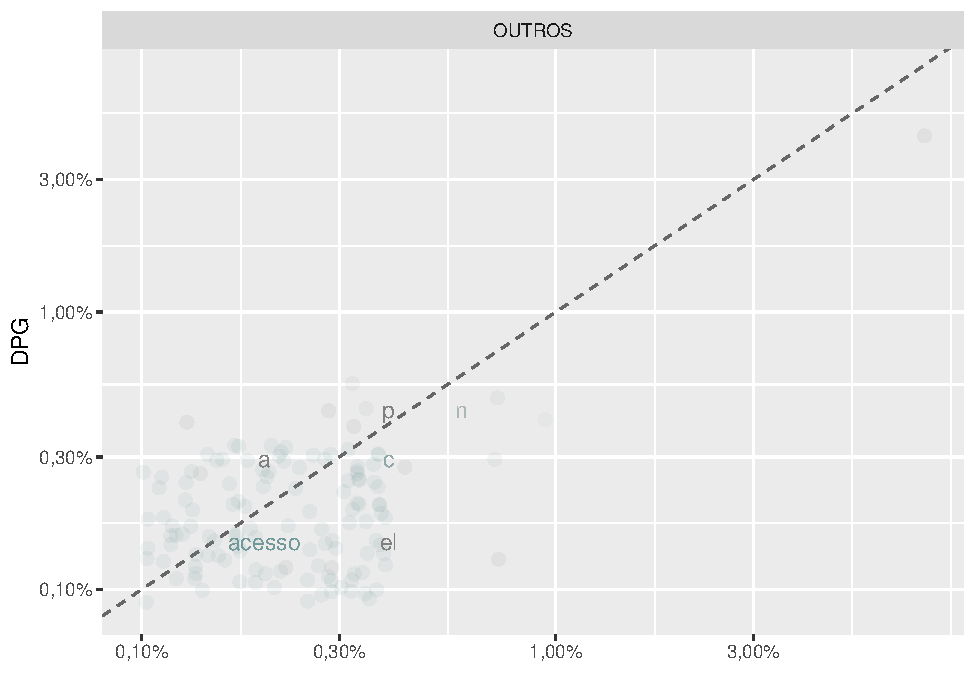
\includegraphics{markdown_v21_files/figure-latex/unnamed-chunk-33-1.pdf}

\begin{Shaded}
\begin{Highlighting}[]
\FunctionTok{Warning messages:}
\FunctionTok{1:}\AttributeTok{ Removed 4450 rows containing missing values (geom_point). }
\FunctionTok{2:}\AttributeTok{ Removed 4451 rows containing missing values (geom_text). }
\end{Highlighting}
\end{Shaded}

\begin{itemize}
\tightlist
\item
  DPG X OUTROS
\end{itemize}

\begin{Shaded}
\begin{Highlighting}[]
\NormalTok{freq09 <-}\StringTok{ }\NormalTok{PROP_PALAVRA }\OperatorTok
\StringTok{    }\KeywordTok{gather}\NormalTok{(DIRETORIA, proportion, }\KeywordTok{c}\NormalTok{(}\StringTok{`}\DataTypeTok{OUTROS}\StringTok{`}\NormalTok{))}
  
  \KeywordTok{library}\NormalTok{(scales)}
  \CommentTok{# expect a warning about rows with missing values being removed}
  \KeywordTok{ggplot}\NormalTok{(freq08, }\KeywordTok{aes}\NormalTok{(}\DataTypeTok{x =}\NormalTok{ proportion, }\DataTypeTok{y =} \StringTok{`}\DataTypeTok{DGC}\StringTok{`}\NormalTok{,}
                        \DataTypeTok{color =} \KeywordTok{abs}\NormalTok{(}\StringTok{`}\DataTypeTok{DGC}\StringTok{`} \OperatorTok{-}\StringTok{ }\NormalTok{proportion))) }\OperatorTok{+}
\StringTok{    }\KeywordTok{geom_abline}\NormalTok{(}\DataTypeTok{color =} \StringTok{"gray40"}\NormalTok{, }\DataTypeTok{lty =} \DecValTok{2}\NormalTok{) }\OperatorTok{+}
\StringTok{    }\KeywordTok{geom_jitter}\NormalTok{(}\DataTypeTok{alpha =} \FloatTok{0.1}\NormalTok{, }\DataTypeTok{size =} \FloatTok{2.5}\NormalTok{, }\DataTypeTok{width =} \FloatTok{0.3}\NormalTok{, }\DataTypeTok{height =} \FloatTok{0.3}\NormalTok{) }\OperatorTok{+}
\StringTok{    }\KeywordTok{geom_text}\NormalTok{(}\KeywordTok{aes}\NormalTok{(}\DataTypeTok{label =}\NormalTok{ palavra), }\DataTypeTok{check_overlap =} \OtherTok{TRUE}\NormalTok{, }\DataTypeTok{vjust =} \FloatTok{1.5}\NormalTok{) }\OperatorTok{+}
\StringTok{    }\KeywordTok{scale_x_log10}\NormalTok{(}\DataTypeTok{labels =} \KeywordTok{percent_format}\NormalTok{(}\DataTypeTok{big.mark =} \StringTok{"."}\NormalTok{, }\DataTypeTok{decimal.mark =} \StringTok{","}\NormalTok{)) }\OperatorTok{+}
\StringTok{    }\KeywordTok{scale_y_log10}\NormalTok{(}\DataTypeTok{labels =} \KeywordTok{percent_format}\NormalTok{(}\DataTypeTok{big.mark =} \StringTok{"."}\NormalTok{, }\DataTypeTok{decimal.mark =} \StringTok{","}\NormalTok{)) }\OperatorTok{+}
\StringTok{    }\KeywordTok{scale_color_gradient}\NormalTok{(}\DataTypeTok{limits =} \KeywordTok{c}\NormalTok{(}\DecValTok{0}\NormalTok{, }\FloatTok{0.001}\NormalTok{),}
                         \DataTypeTok{low =} \StringTok{"darkslategray4"}\NormalTok{, }\DataTypeTok{high =} \StringTok{"gray75"}\NormalTok{) }\OperatorTok{+}
\StringTok{    }\KeywordTok{facet_wrap}\NormalTok{(}\OperatorTok{~}\NormalTok{DIRETORIA, }\DataTypeTok{ncol =} \DecValTok{1}\NormalTok{) }\OperatorTok{+}
\StringTok{    }\KeywordTok{theme}\NormalTok{(}\DataTypeTok{legend.position=}\StringTok{"none"}\NormalTok{) }\OperatorTok{+}
\StringTok{    }\KeywordTok{labs}\NormalTok{(}\DataTypeTok{y =} \StringTok{"DGC"}\NormalTok{, }\DataTypeTok{x =} \OtherTok{NULL}\NormalTok{)}
\end{Highlighting}
\end{Shaded}

\begin{verbatim}
## Warning: Removed 4302 rows containing missing values (geom_point).
\end{verbatim}

\begin{verbatim}
## Warning: Removed 4303 rows containing missing values (geom_text).
\end{verbatim}

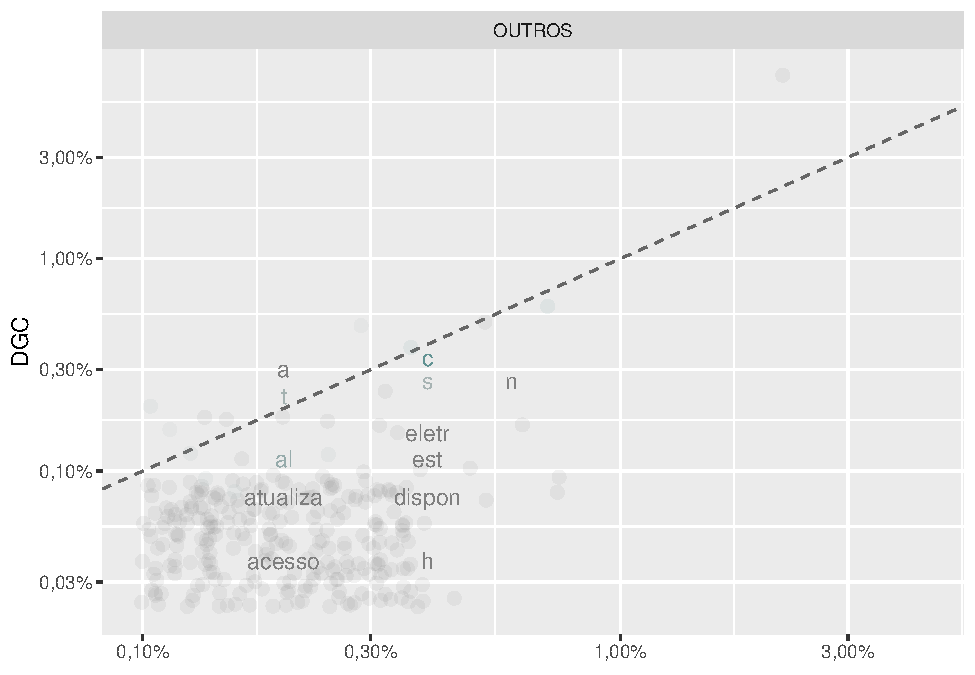
\includegraphics{markdown_v21_files/figure-latex/unnamed-chunk-34-1.pdf}

\begin{Shaded}
\begin{Highlighting}[]
\FunctionTok{Warning messages:}
\FunctionTok{1:}\AttributeTok{ Removed 4302 rows containing missing values (geom_point). }
\FunctionTok{2:}\AttributeTok{ Removed 4303 rows containing missing values (geom_text).}
\end{Highlighting}
\end{Shaded}

\begin{itemize}
\tightlist
\item
  Zipf's law
\end{itemize}

\begin{Shaded}
\begin{Highlighting}[]
\NormalTok{freq_by_rank <-}\StringTok{ }\NormalTok{diretoria_palavras }\OperatorTok
\KeywordTok{group_by}\NormalTok{(DIRETORIA) }\OperatorTok
\KeywordTok{mutate}\NormalTok{(}\DataTypeTok{ranque =} \KeywordTok{row_number}\NormalTok{(),}
\StringTok{`}\DataTypeTok{frequência de termos}\StringTok{`}\NormalTok{ =}\StringTok{ }\NormalTok{n}\OperatorTok{/}\NormalTok{total_palavras)}

\CommentTok{# Plot}
\NormalTok{freq_by_rank }\OperatorTok
\KeywordTok{ggplot}\NormalTok{(}\KeywordTok{aes}\NormalTok{(ranque, }\StringTok{`}\DataTypeTok{frequência de termos}\StringTok{`}\NormalTok{, }\DataTypeTok{color =}\NormalTok{ DIRETORIA)) }\OperatorTok{+}
\KeywordTok{geom_abline}\NormalTok{(}\DataTypeTok{intercept =} \OperatorTok{-}\FloatTok{0.62}\NormalTok{, }\DataTypeTok{slope =} \OperatorTok{-}\FloatTok{1.1}\NormalTok{, }\DataTypeTok{color =} \StringTok{"gray50"}\NormalTok{, }\DataTypeTok{linetype =} \DecValTok{2}\NormalTok{) }\OperatorTok{+}
\KeywordTok{geom_line}\NormalTok{(}\DataTypeTok{size =} \FloatTok{1.1}\NormalTok{, }\DataTypeTok{alpha =} \FloatTok{0.8}\NormalTok{, }\DataTypeTok{show.legend =} \OtherTok{TRUE}\NormalTok{) }\OperatorTok{+}
\KeywordTok{scale_x_log10}\NormalTok{(}\DataTypeTok{labels=}\NormalTok{gcomma) }\OperatorTok{+}
\KeywordTok{scale_y_log10}\NormalTok{(}\DataTypeTok{labels=}\NormalTok{gcomma)}
\end{Highlighting}
\end{Shaded}

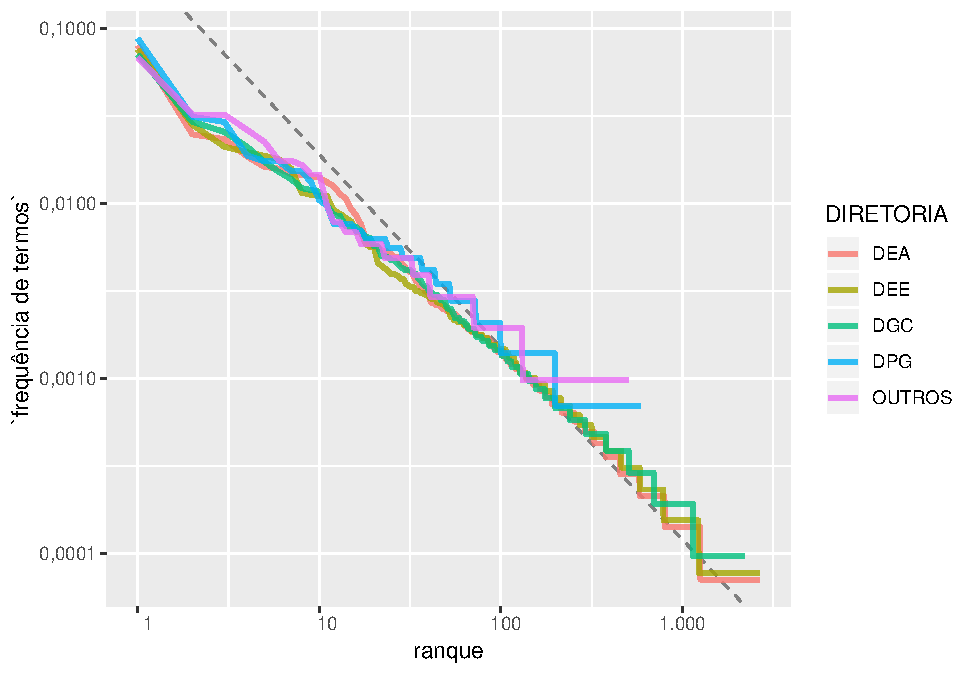
\includegraphics{markdown_v21_files/figure-latex/unnamed-chunk-35-1.pdf}

\paragraph{Frequência de palavras por
diretoria}\label{frequencia-de-palavras-por-diretoria}

\begin{Shaded}
\begin{Highlighting}[]
\NormalTok{diretoria_palavras <-}\StringTok{ }\NormalTok{DB }\OperatorTok
\StringTok{  }\KeywordTok{unnest_tokens}\NormalTok{(palavra, DESCRI_PEDIDO) }\OperatorTok
\StringTok{  }\KeywordTok{count}\NormalTok{(DIRETORIA, palavra, }\DataTypeTok{sort =} \OtherTok{TRUE}\NormalTok{) }\OperatorTok
\StringTok{  }\KeywordTok{ungroup}\NormalTok{()}
\CommentTok{#diretoria_palavras}

\NormalTok{plot_diretoria_palavras <-}\StringTok{ }\NormalTok{diretoria_palavras }\OperatorTok
\StringTok{  }\KeywordTok{bind_tf_idf}\NormalTok{(palavra, DIRETORIA, n) }\OperatorTok
\StringTok{  }\KeywordTok{arrange}\NormalTok{(}\KeywordTok{desc}\NormalTok{(tf_idf)) }\OperatorTok
\StringTok{  }\KeywordTok{mutate}\NormalTok{(}\DataTypeTok{palavra =} \KeywordTok{factor}\NormalTok{(palavra, }\DataTypeTok{levels =} \KeywordTok{rev}\NormalTok{(}\KeywordTok{unique}\NormalTok{(palavra)))) }\OperatorTok
\StringTok{  }\KeywordTok{mutate}\NormalTok{(}\DataTypeTok{DIRETORIA =} \KeywordTok{factor}\NormalTok{(DIRETORIA, }\DataTypeTok{levels =} \KeywordTok{c}\NormalTok{(}\StringTok{"DEA"}\NormalTok{,}
                                                  \StringTok{"DEE"}\NormalTok{,}
                                                  \StringTok{"DGC"}\NormalTok{,}
                                                  \StringTok{"DPG"}\NormalTok{,}
                                                  \StringTok{"OUTROS"}\NormalTok{)))}
\CommentTok{#View(head(plot_diretoria_palavras))}
\CommentTok{#jpeg("02_freq_palavras_dir.jpeg")}
\NormalTok{plot_diretoria_palavras }\OperatorTok
\KeywordTok{group_by}\NormalTok{(DIRETORIA) }\OperatorTok
\KeywordTok{top_n}\NormalTok{(}\DecValTok{10}\NormalTok{, tf_idf) }\OperatorTok
\KeywordTok{ungroup}\NormalTok{() }\OperatorTok
\KeywordTok{mutate}\NormalTok{(}\DataTypeTok{palavra =} \KeywordTok{reorder}\NormalTok{(palavra, tf_idf)) }\OperatorTok
\KeywordTok{ggplot}\NormalTok{(}\KeywordTok{aes}\NormalTok{(palavra, tf_idf, }\DataTypeTok{fill =}\NormalTok{ DIRETORIA)) }\OperatorTok{+}
\KeywordTok{geom_col}\NormalTok{(}\DataTypeTok{show.legend =} \OtherTok{FALSE}\NormalTok{) }\OperatorTok{+}
\KeywordTok{labs}\NormalTok{(}\DataTypeTok{x =} \OtherTok{NULL}\NormalTok{, }\DataTypeTok{y =} \StringTok{"tf-idf"}\NormalTok{) }\OperatorTok{+}
\KeywordTok{facet_wrap}\NormalTok{(}\OperatorTok{~}\NormalTok{DIRETORIA, }\DataTypeTok{ncol =} \DecValTok{2}\NormalTok{, }\DataTypeTok{scales =} \StringTok{"free"}\NormalTok{) }\OperatorTok{+}
\KeywordTok{coord_flip}\NormalTok{() }\OperatorTok{+}\StringTok{ }
\KeywordTok{scale_y_continuous}\NormalTok{(}\DataTypeTok{labels=}\NormalTok{gcomma)}
\end{Highlighting}
\end{Shaded}

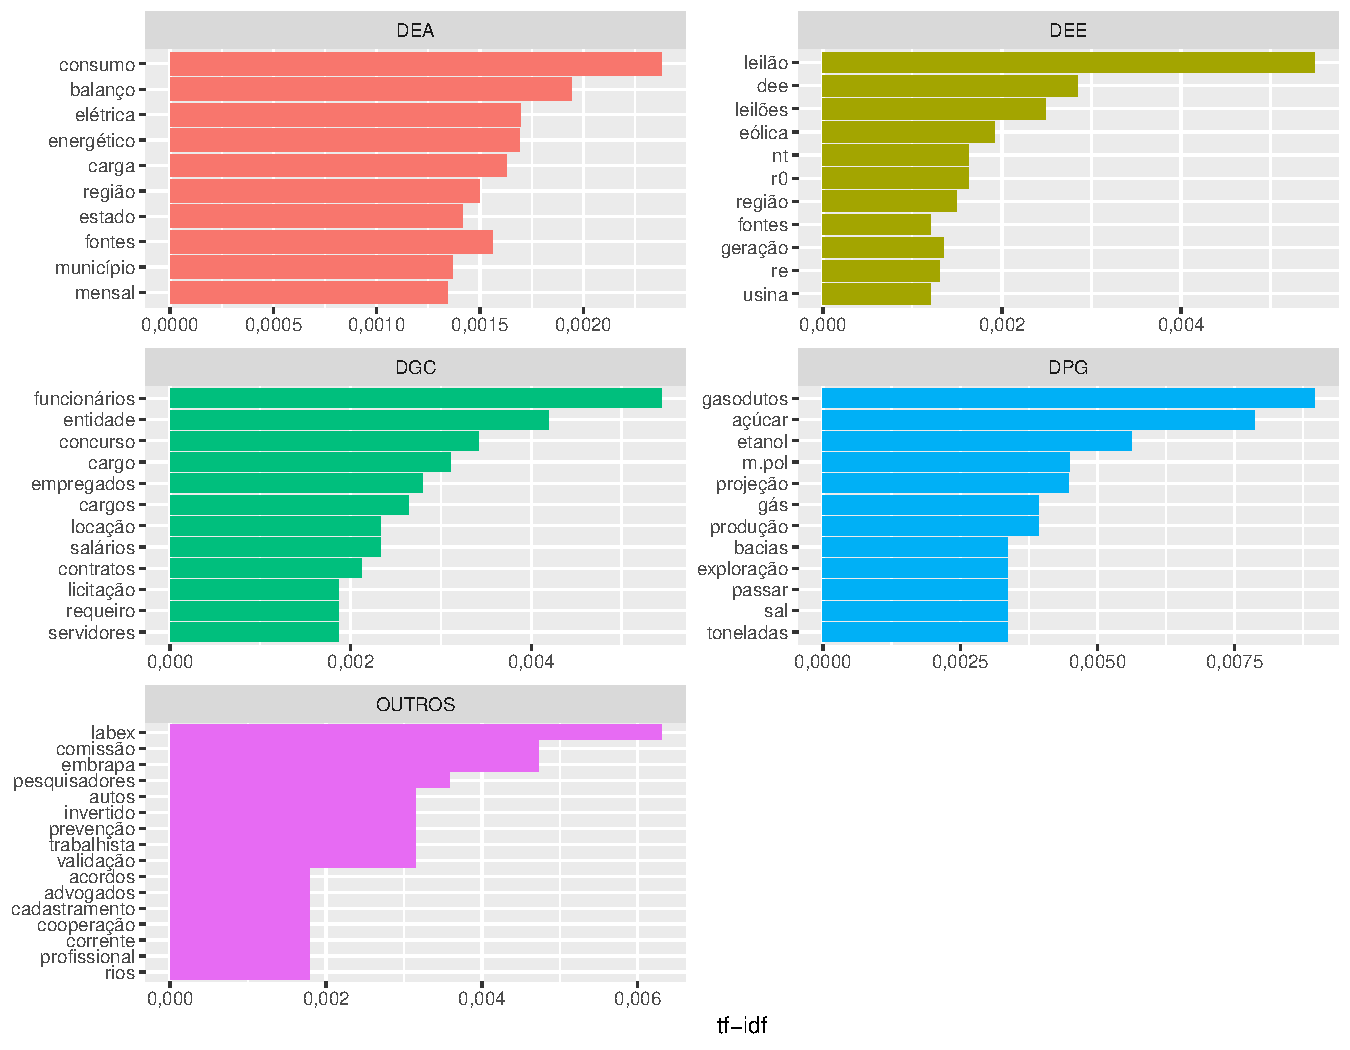
\includegraphics{markdown_v21_files/figure-latex/02_freq_palavras_dir-1.pdf}

\begin{Shaded}
\begin{Highlighting}[]
\CommentTok{#dev.off()}
\end{Highlighting}
\end{Shaded}

\paragraph{Filtrando um pedaço de
texto}\label{filtrando-um-pedaco-de-texto}

\begin{Shaded}
\begin{Highlighting}[]
\NormalTok{DB }\OperatorTok
\KeywordTok{filter}\NormalTok{(}\KeywordTok{str_detect}\NormalTok{(DESCRI_PEDIDO, }\StringTok{"r0"}\NormalTok{)) }\OperatorTok
\KeywordTok{select}\NormalTok{(DESCRI_PEDIDO) }\OperatorTok
\StringTok{  }\KeywordTok{head}\NormalTok{()}
\end{Highlighting}
\end{Shaded}

\begin{verbatim}
##                                                                                                                                                                                                                                                                                                                                                                                                                                                                                                                                                 DESCRI_PEDIDO
## 1                                                                                                                                                                                                                                                                          Prezados,\n\nSolicitamos que o deck do Newave 22.6 utilizado para Revisão da Garantia Física de UHEs, conforme consta da Nota Técnica EPE-DEE-RE-097/2016-r0 da Empresa de Pesquisa Energética -  EPE, nos seja enviado para conhecimento, por gentileza.\n\nObrigada,\nGraziella.
## 2                                                                                                                                                                                                                                                                                                                                                                                                                                                        Gostaria de ter acesso à Nota Técnica EPE-DEE-RE-097/2016-r0, pois não a encontro disponível online.
## 3 Solicitamos para nossa análise cópias dos relatórios nºs EPE-DEE-RE-147/2008-r0 que trata dos ESTUDOS RELATIVOS AOS GRANDES APROVEITAMENTOS HIDRELÉTRICOS NA REGIÃO AMAZÔNICA – Análise do sistema de atendimento aos estados do Acre e Rondônia no período Pré-Madeira – dezembro de 2008 e do relatório nº RE-EPES–4.010/08, que trata do SISTEMA ACRE-RONDÔNIA R2 – Estudos de Transitórios Eletromagnéticos e Condutor Econômico das LTs 230 kV P.Velho – Abunã – Rio Branco – janeiro de 2009.\n\nAgradecemos breve retorno.\n\nAtt.\n\nMônica\n\n\n\n
## 4                                                                                                                                                                                                                                                                                                                                                                            Cópia do documento EPE-DEE-RE-083/2010-r0, “Estudo de Integração das Usinas Hidrelétricas Previstas para o Estado de Santa Catarina”, elaborado pela EPE em novembro de 2010. \n
## 5                                                                                                                                                                                                                                                                                                                                                                                                                                                                                                       Solicito cópia da Nota Técnica EPE-DEE-RE-097/2016-r0
## 6                                                                                                                                                                                                                                                                                                                                                                                                          Bom dia, por gentileza gostaria ter acesso ao parecer técnico EPE-DEE-PT-051/2016-r0 e projeto alternativo apresentado pela tecnogera.\n\nObrigada
\end{verbatim}

Uma limpeza removendo palavras sem significado semântico
(\textbf{stopwords}) pode auxiliar o algoritmo a retornar palavras ainda
mais acertivas

\subsubsection{Radicais}\label{radicais}

Podemos diminuir redundâncias por parte do algoritmo ensinando-o a
compreender palavras que podem estar escritas de forma diferente mas que
em significado semântico são semelhantes. Para isso, analisamos o
radical de palavras com um mesmo prefixo mas com sufixos diferentes seja
por quisistos como gênero ou plural.

Exemplos:

leilão \(\propto\) leilões estado \(\propto\) estados região \(\propto\)
regiões

\texttt{Falta\ implementar}

\subsubsection{Stopwords}\label{stopwords}

Com o arquivo de \texttt{stopwords}previamente inserido vamos,
primeiramente, transforma-lo em um data\_frame a fim de futuramente
utilizá-lo para extrair do texto palavras em comum.

\paragraph{\texorpdfstring{Freq. de palavras sem \textbf{stopwords} por
diretoria}{Freq. de palavras sem stopwords por diretoria}}\label{freq.-de-palavras-sem-stopwords-por-diretoria}

\begin{Shaded}
\begin{Highlighting}[]
\NormalTok{mystopwords <-}\StringTok{ }\KeywordTok{data_frame}\NormalTok{(}\DataTypeTok{palavra =}\NormalTok{ stopwords_pt)}
\end{Highlighting}
\end{Shaded}

\begin{verbatim}
## Warning: `data_frame()` is deprecated, use `tibble()`.
## This warning is displayed once per session.
\end{verbatim}

\begin{Shaded}
\begin{Highlighting}[]
\NormalTok{diretoria_palavras_noSTOP <-}\StringTok{ }\KeywordTok{anti_join}\NormalTok{(diretoria_palavras, mystopwords, }\DataTypeTok{by =} \StringTok{"palavra"}\NormalTok{)}
\CommentTok{#View(head(diretoria_palavras_noSTOP))}
\end{Highlighting}
\end{Shaded}

\begin{Shaded}
\begin{Highlighting}[]
\CommentTok{#diretoria_palavras_noSTOP_noSTOP}
\NormalTok{plot_diretoria_palavras_noSTOP <-}\StringTok{ }\NormalTok{diretoria_palavras_noSTOP }\OperatorTok
\StringTok{  }\KeywordTok{bind_tf_idf}\NormalTok{(palavra, DIRETORIA, n) }\OperatorTok
\StringTok{  }\KeywordTok{arrange}\NormalTok{(}\KeywordTok{desc}\NormalTok{(tf_idf)) }\OperatorTok
\StringTok{  }\KeywordTok{mutate}\NormalTok{(}\DataTypeTok{word =} \KeywordTok{factor}\NormalTok{(palavra, }\DataTypeTok{levels =} \KeywordTok{rev}\NormalTok{(}\KeywordTok{unique}\NormalTok{(palavra)))) }\OperatorTok
\StringTok{  }\KeywordTok{mutate}\NormalTok{(}\DataTypeTok{DIRETORIA =} \KeywordTok{factor}\NormalTok{(DIRETORIA, }\DataTypeTok{levels =} \KeywordTok{c}\NormalTok{(}\StringTok{"DEA"}\NormalTok{,}
                                                  \StringTok{"DEE"}\NormalTok{,}
                                                  \StringTok{"DGC"}\NormalTok{,}
                                                  \StringTok{"DPG"}\NormalTok{,}
                                                  \StringTok{"OUTROS"}\NormalTok{)))}
\CommentTok{#plot_diretoria_palavras_noSTOP}
\CommentTok{#windows.options(width=10, height=10)}
\CommentTok{#jpeg("03_freq_palavras_dir_nostop.jpeg")}
\NormalTok{plot_diretoria_palavras_noSTOP }\OperatorTok
\KeywordTok{group_by}\NormalTok{(DIRETORIA) }\OperatorTok
\KeywordTok{top_n}\NormalTok{(}\DecValTok{10}\NormalTok{, tf_idf) }\OperatorTok
\KeywordTok{ungroup}\NormalTok{() }\OperatorTok
\KeywordTok{mutate}\NormalTok{(}\DataTypeTok{palavra =} \KeywordTok{reorder}\NormalTok{(palavra, tf_idf)) }\OperatorTok
\KeywordTok{ggplot}\NormalTok{(}\KeywordTok{aes}\NormalTok{(palavra, tf_idf, }\DataTypeTok{fill =}\NormalTok{ DIRETORIA)) }\OperatorTok{+}
\KeywordTok{geom_col}\NormalTok{(}\DataTypeTok{show.legend =} \OtherTok{FALSE}\NormalTok{) }\OperatorTok{+}
\KeywordTok{labs}\NormalTok{(}\DataTypeTok{x =} \OtherTok{NULL}\NormalTok{, }\DataTypeTok{y =} \StringTok{"tf-idf"}\NormalTok{) }\OperatorTok{+}
\KeywordTok{facet_wrap}\NormalTok{(}\OperatorTok{~}\NormalTok{DIRETORIA, }\DataTypeTok{ncol =} \DecValTok{2}\NormalTok{, }\DataTypeTok{scales =} \StringTok{"free"}\NormalTok{) }\OperatorTok{+}
\KeywordTok{coord_flip}\NormalTok{() }\OperatorTok{+}\StringTok{ }
\KeywordTok{scale_y_continuous}\NormalTok{(}\DataTypeTok{labels=}\NormalTok{gcomma)}
\end{Highlighting}
\end{Shaded}

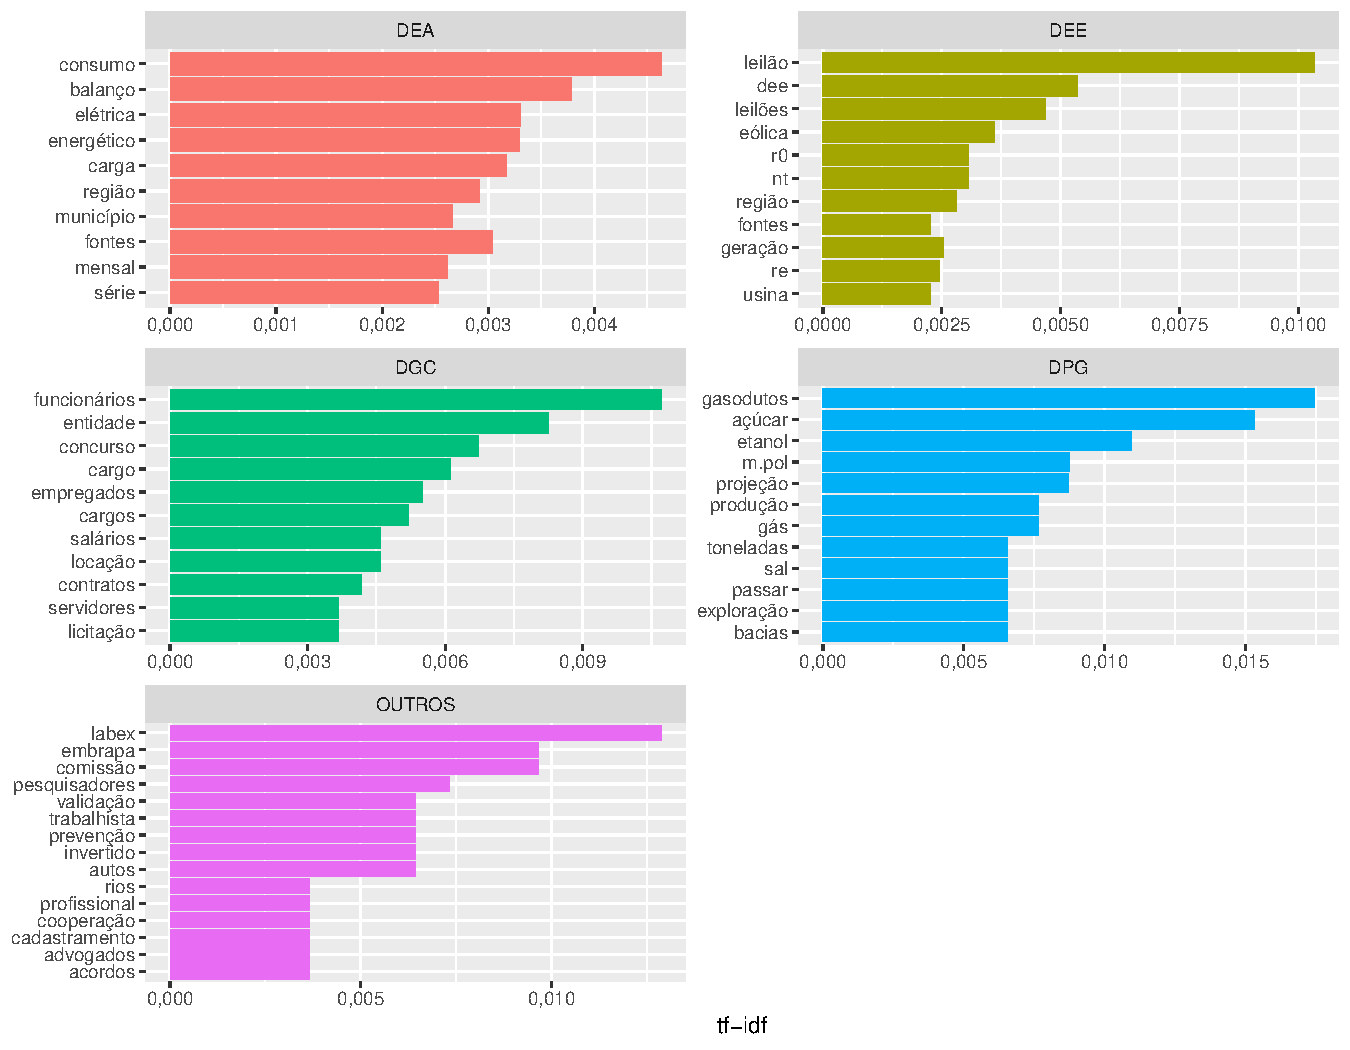
\includegraphics{markdown_v21_files/figure-latex/03_freq_palavras_dir_nostop-1.pdf}

\begin{Shaded}
\begin{Highlighting}[]
\CommentTok{#dev.off()}
\end{Highlighting}
\end{Shaded}

\subsubsection{Usando bigram para n=2 palavras por
token}\label{usando-bigram-para-n2-palavras-por-token}

\paragraph{Frequência de palavras por
diretoria}\label{frequencia-de-palavras-por-diretoria-1}

\begin{Shaded}
\begin{Highlighting}[]
\NormalTok{diretoria_palavras_bigram <-}\StringTok{ }\NormalTok{DB }\OperatorTok
\StringTok{  }\KeywordTok{select}\NormalTok{(DESCRI_PEDIDO,DIRETORIA) }\OperatorTok
\StringTok{  }\KeywordTok{unnest_tokens}\NormalTok{(BIGRAM, DESCRI_PEDIDO, }\DataTypeTok{token =} \StringTok{"ngrams"}\NormalTok{, }\DataTypeTok{n =} \DecValTok{2}\NormalTok{) }\OperatorTok
\StringTok{  }\KeywordTok{count}\NormalTok{(DIRETORIA, BIGRAM, }\DataTypeTok{sort =} \OtherTok{TRUE}\NormalTok{) }\OperatorTok
\StringTok{  }\KeywordTok{ungroup}\NormalTok{()}
\CommentTok{#diretoria_palavras_bigram}

\NormalTok{plot_diretoria_palavras_bigram <-}\StringTok{ }\NormalTok{diretoria_palavras_bigram }\OperatorTok
\StringTok{  }\KeywordTok{bind_tf_idf}\NormalTok{(BIGRAM, DIRETORIA, n) }\OperatorTok
\StringTok{  }\KeywordTok{arrange}\NormalTok{(}\KeywordTok{desc}\NormalTok{(tf_idf)) }\OperatorTok
\StringTok{  }\KeywordTok{mutate}\NormalTok{(}\DataTypeTok{BIGRAM =} \KeywordTok{factor}\NormalTok{(BIGRAM, }\DataTypeTok{levels =} \KeywordTok{rev}\NormalTok{(}\KeywordTok{unique}\NormalTok{(BIGRAM)))) }\OperatorTok
\StringTok{  }\KeywordTok{mutate}\NormalTok{(}\DataTypeTok{DIRETORIA =} \KeywordTok{factor}\NormalTok{(DIRETORIA, }\DataTypeTok{levels =} \KeywordTok{c}\NormalTok{(}\StringTok{"DEA"}\NormalTok{,}
                                                  \StringTok{"DEE"}\NormalTok{,}
                                                  \StringTok{"DGC"}\NormalTok{,}
                                                  \StringTok{"DPG"}\NormalTok{,}
                                                  \StringTok{"OUTROS"}\NormalTok{)))}
\CommentTok{#View(head(plot_diretoria_palavras_bigram))}
\CommentTok{#jpeg("02_freq_palavras_dir.jpeg")}
\NormalTok{plot_diretoria_palavras_bigram }\OperatorTok
\KeywordTok{group_by}\NormalTok{(DIRETORIA) }\OperatorTok
\KeywordTok{top_n}\NormalTok{(}\DecValTok{10}\NormalTok{, tf_idf) }\OperatorTok
\KeywordTok{ungroup}\NormalTok{() }\OperatorTok
\KeywordTok{mutate}\NormalTok{(}\DataTypeTok{BIGRAM =} \KeywordTok{reorder}\NormalTok{(BIGRAM, tf_idf)) }\OperatorTok
\KeywordTok{ggplot}\NormalTok{(}\KeywordTok{aes}\NormalTok{(BIGRAM, tf_idf, }\DataTypeTok{fill =}\NormalTok{ DIRETORIA)) }\OperatorTok{+}
\KeywordTok{geom_col}\NormalTok{(}\DataTypeTok{show.legend =} \OtherTok{FALSE}\NormalTok{) }\OperatorTok{+}
\KeywordTok{labs}\NormalTok{(}\DataTypeTok{x =} \OtherTok{NULL}\NormalTok{, }\DataTypeTok{y =} \StringTok{"tf-idf"}\NormalTok{) }\OperatorTok{+}
\KeywordTok{facet_wrap}\NormalTok{(}\OperatorTok{~}\NormalTok{DIRETORIA, }\DataTypeTok{ncol =} \DecValTok{2}\NormalTok{, }\DataTypeTok{scales =} \StringTok{"free"}\NormalTok{) }\OperatorTok{+}
\KeywordTok{coord_flip}\NormalTok{() }\OperatorTok{+}\StringTok{ }
\KeywordTok{scale_y_continuous}\NormalTok{(}\DataTypeTok{labels=}\NormalTok{gcomma)}
\end{Highlighting}
\end{Shaded}

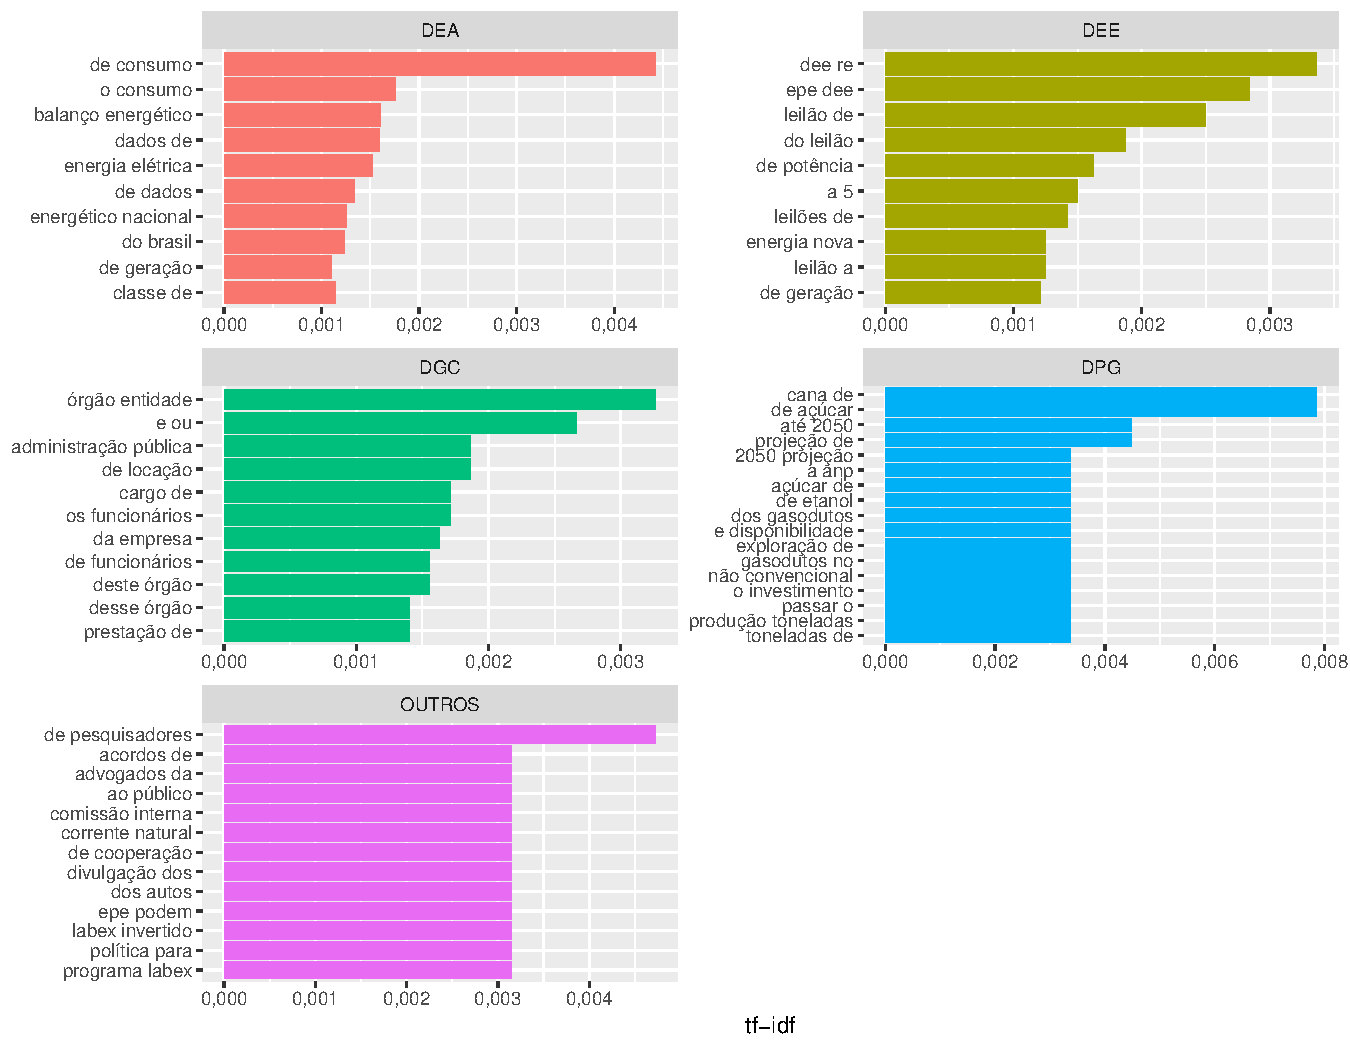
\includegraphics{markdown_v21_files/figure-latex/03_freq_palavras_dir-1.pdf}

\begin{Shaded}
\begin{Highlighting}[]
\CommentTok{#dev.off()}
\end{Highlighting}
\end{Shaded}

\subsubsection{Usando bigram para n=3 palavras por
token}\label{usando-bigram-para-n3-palavras-por-token}

\paragraph{Frequência de palavras por
diretoria}\label{frequencia-de-palavras-por-diretoria-2}

\begin{Shaded}
\begin{Highlighting}[]
\NormalTok{diretoria_palavras_trigram <-}\StringTok{ }\NormalTok{DB }\OperatorTok
\StringTok{  }\KeywordTok{select}\NormalTok{(DESCRI_PEDIDO,DIRETORIA) }\OperatorTok
\StringTok{  }\KeywordTok{unnest_tokens}\NormalTok{(TRIGRAM, DESCRI_PEDIDO, }\DataTypeTok{token =} \StringTok{"ngrams"}\NormalTok{, }\DataTypeTok{n =} \DecValTok{3}\NormalTok{) }\OperatorTok
\StringTok{  }\KeywordTok{count}\NormalTok{(DIRETORIA, TRIGRAM, }\DataTypeTok{sort =} \OtherTok{TRUE}\NormalTok{) }\OperatorTok
\StringTok{  }\KeywordTok{ungroup}\NormalTok{()}
\CommentTok{#diretoria_palavras_trigram}

\NormalTok{plot_diretoria_palavras_trigram <-}\StringTok{ }\NormalTok{diretoria_palavras_trigram }\OperatorTok
\StringTok{  }\KeywordTok{bind_tf_idf}\NormalTok{(TRIGRAM, DIRETORIA, n) }\OperatorTok
\StringTok{  }\KeywordTok{arrange}\NormalTok{(}\KeywordTok{desc}\NormalTok{(tf_idf)) }\OperatorTok
\StringTok{  }\KeywordTok{mutate}\NormalTok{(}\DataTypeTok{TRIGRAM =} \KeywordTok{factor}\NormalTok{(TRIGRAM, }\DataTypeTok{levels =} \KeywordTok{rev}\NormalTok{(}\KeywordTok{unique}\NormalTok{(TRIGRAM)))) }\OperatorTok
\StringTok{  }\KeywordTok{mutate}\NormalTok{(}\DataTypeTok{DIRETORIA =} \KeywordTok{factor}\NormalTok{(DIRETORIA, }\DataTypeTok{levels =} \KeywordTok{c}\NormalTok{(}\StringTok{"DEA"}\NormalTok{,}
                                                  \StringTok{"DEE"}\NormalTok{,}
                                                  \StringTok{"DGC"}\NormalTok{,}
                                                  \StringTok{"DPG"}\NormalTok{,}
                                                  \StringTok{"OUTROS"}\NormalTok{)))}
\CommentTok{#View(head(plot_diretoria_palavras_trigram))}
\CommentTok{#jpeg("02_freq_palavras_dir.jpeg")}
\NormalTok{plot_diretoria_palavras_trigram }\OperatorTok
\KeywordTok{group_by}\NormalTok{(DIRETORIA) }\OperatorTok
\KeywordTok{top_n}\NormalTok{(}\DecValTok{10}\NormalTok{, tf_idf) }\OperatorTok
\KeywordTok{ungroup}\NormalTok{() }\OperatorTok
\KeywordTok{mutate}\NormalTok{(}\DataTypeTok{TRIGRAM =} \KeywordTok{reorder}\NormalTok{(TRIGRAM, tf_idf)) }\OperatorTok
\KeywordTok{ggplot}\NormalTok{(}\KeywordTok{aes}\NormalTok{(TRIGRAM, tf_idf, }\DataTypeTok{fill =}\NormalTok{ DIRETORIA)) }\OperatorTok{+}
\KeywordTok{geom_col}\NormalTok{(}\DataTypeTok{show.legend =} \OtherTok{FALSE}\NormalTok{) }\OperatorTok{+}
\KeywordTok{labs}\NormalTok{(}\DataTypeTok{x =} \OtherTok{NULL}\NormalTok{, }\DataTypeTok{y =} \StringTok{"tf-idf"}\NormalTok{) }\OperatorTok{+}
\KeywordTok{facet_wrap}\NormalTok{(}\OperatorTok{~}\NormalTok{DIRETORIA, }\DataTypeTok{ncol =} \DecValTok{2}\NormalTok{, }\DataTypeTok{scales =} \StringTok{"free"}\NormalTok{) }\OperatorTok{+}
\KeywordTok{coord_flip}\NormalTok{() }\OperatorTok{+}\StringTok{ }
\KeywordTok{scale_y_continuous}\NormalTok{(}\DataTypeTok{labels=}\NormalTok{gcomma)}
\end{Highlighting}
\end{Shaded}

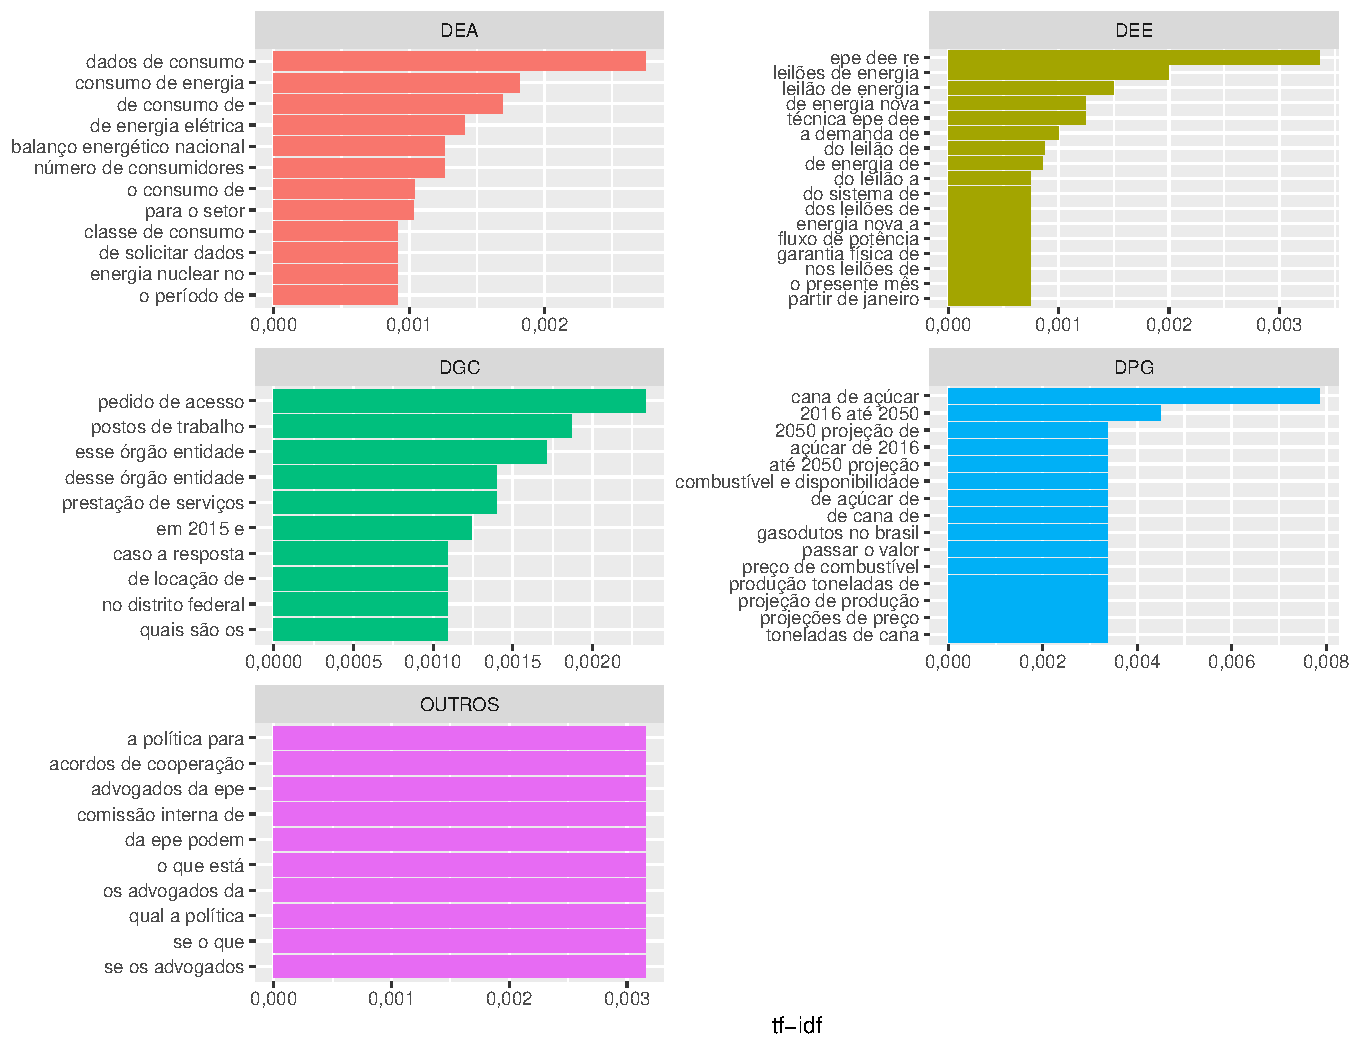
\includegraphics{markdown_v21_files/figure-latex/04_freq_palavras_dir-1.pdf}

\begin{Shaded}
\begin{Highlighting}[]
\CommentTok{#dev.off()}
\end{Highlighting}
\end{Shaded}

\subsection{tidy object into document-term
matrix}\label{tidy-object-into-document-term-matrix}

\begin{Shaded}
\begin{Highlighting}[]
\NormalTok{plot_diretoria_palavras <-}\StringTok{ }\NormalTok{diretoria_palavras }\OperatorTok
\StringTok{  }\KeywordTok{bind_tf_idf}\NormalTok{(palavra, DIRETORIA, n) }\OperatorTok
\StringTok{  }\KeywordTok{arrange}\NormalTok{(}\KeywordTok{desc}\NormalTok{(tf_idf)) }\OperatorTok
\StringTok{  }\KeywordTok{mutate}\NormalTok{(}\DataTypeTok{palavra =} \KeywordTok{factor}\NormalTok{(palavra, }\DataTypeTok{levels =} \KeywordTok{rev}\NormalTok{(}\KeywordTok{unique}\NormalTok{(palavra)))) }\OperatorTok
\StringTok{  }\KeywordTok{mutate}\NormalTok{(}\DataTypeTok{DIRETORIA =} \KeywordTok{factor}\NormalTok{(DIRETORIA, }\DataTypeTok{levels =} \KeywordTok{c}\NormalTok{(}\StringTok{"DEA"}\NormalTok{,}
                                                  \StringTok{"DEE"}\NormalTok{,}
                                                  \StringTok{"DGC"}\NormalTok{,}
                                                  \StringTok{"DPG"}\NormalTok{,}
                                                  \StringTok{"OUTROS"}\NormalTok{)))}

\NormalTok{dtm =}\StringTok{ }\NormalTok{plot_diretoria_palavras }\OperatorTok
\KeywordTok{cast_dtm}\NormalTok{(}\DataTypeTok{document =}\NormalTok{ DIRETORIA, }\DataTypeTok{term =}\NormalTok{ palavra, n)}
\end{Highlighting}
\end{Shaded}

\subsubsection{Nuvem de palavras}\label{nuvem-de-palavras}

\paragraph{Nuvem de palavras por diretoria - s/ steeming e/ c/ stopwords
-
onegram}\label{nuvem-de-palavras-por-diretoria---s-steeming-e-c-stopwords---onegram}

\begin{Shaded}
\begin{Highlighting}[]
\CommentTok{#View(head(plot_diretoria_palavras))}
\KeywordTok{library}\NormalTok{(wordcloud)}
\NormalTok{plot_diretorias_tf_dif =}\StringTok{ }\NormalTok{plot_diretoria_palavras }\OperatorTok
\StringTok{    }\KeywordTok{select}\NormalTok{(palavra, tf_idf, DIRETORIA) }\OperatorTok
\StringTok{    }\KeywordTok{mutate}\NormalTok{(}\DataTypeTok{palavra =} \KeywordTok{reorder}\NormalTok{(palavra, tf_idf))}

\NormalTok{## DEE}
\CommentTok{#jpeg("XX_wordclou_tfidf_dir01_DEE.jpeg")}
\NormalTok{nuvem1 =}\StringTok{ }
\NormalTok{plot_diretorias_tf_dif }\OperatorTok
\StringTok{  }\KeywordTok{filter}\NormalTok{(DIRETORIA }\OperatorTok{==}\StringTok{ "DEE"}\NormalTok{) }\OperatorTok
\StringTok{  }\KeywordTok{select}\NormalTok{(}\OperatorTok{-}\NormalTok{DIRETORIA, }\DataTypeTok{word =}\NormalTok{ palavra,}\DataTypeTok{freq =}\NormalTok{ tf_idf) }\OperatorTok
\StringTok{  }\CommentTok{#top_n(150, freq) %>%}
\StringTok{  }\KeywordTok{as.data.frame}\NormalTok{() }

\KeywordTok{set.seed}\NormalTok{(}\DecValTok{231321}\NormalTok{)}
\KeywordTok{wordcloud}\NormalTok{(}\DataTypeTok{words =}\NormalTok{ nuvem1}\OperatorTok{$}\NormalTok{word, }\DataTypeTok{freq =}\NormalTok{ nuvem1}\OperatorTok{$}\NormalTok{freq, }\DataTypeTok{min.freq =} \FloatTok{0.2}\NormalTok{,}
          \DataTypeTok{max.words=}\DecValTok{250}\NormalTok{, }\DataTypeTok{random.order=}\OtherTok{FALSE}\NormalTok{, }\DataTypeTok{rot.per=}\FloatTok{0.35}\NormalTok{, }
          \DataTypeTok{colors=}\KeywordTok{brewer.pal}\NormalTok{(}\DecValTok{10}\NormalTok{, }\StringTok{"Dark2"}\NormalTok{))}
\end{Highlighting}
\end{Shaded}

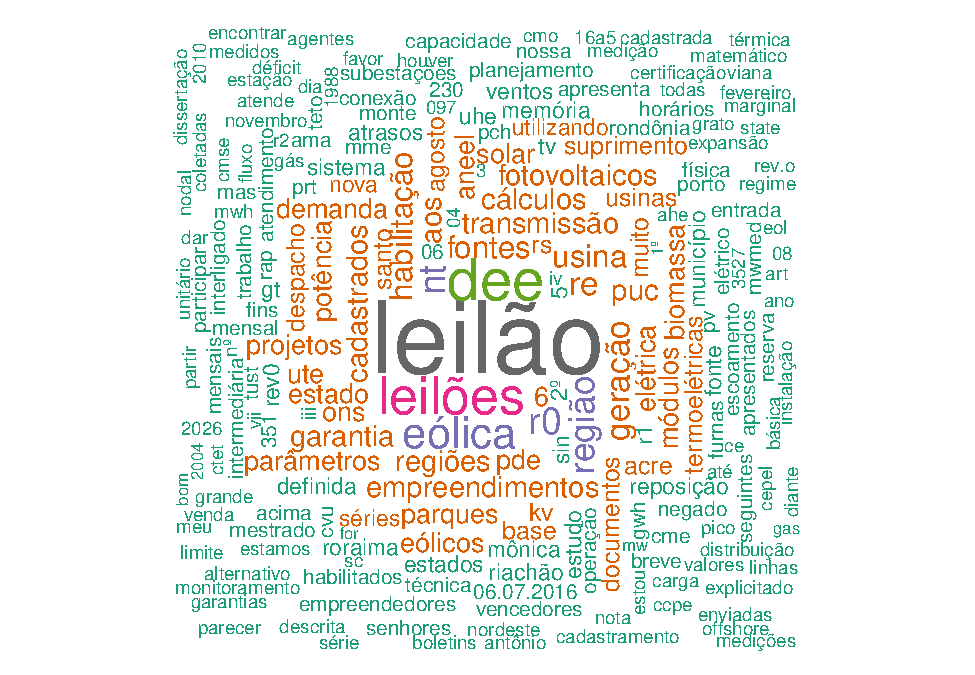
\includegraphics{markdown_v21_files/figure-latex/unnamed-chunk-39-1.pdf}

\begin{Shaded}
\begin{Highlighting}[]
\NormalTok{## DGC}
\CommentTok{#jpeg("XX_wordclou_tfidf_dir02_DGC.jpeg")}
\NormalTok{nuvem2 =}\StringTok{ }
\NormalTok{plot_diretorias_tf_dif }\OperatorTok
\StringTok{  }\KeywordTok{filter}\NormalTok{(DIRETORIA }\OperatorTok{==}\StringTok{ "DGC"}\NormalTok{) }\OperatorTok
\StringTok{  }\KeywordTok{select}\NormalTok{(}\OperatorTok{-}\NormalTok{DIRETORIA, }\DataTypeTok{word =}\NormalTok{ palavra,}\DataTypeTok{freq =}\NormalTok{ tf_idf) }\OperatorTok
\StringTok{  }\CommentTok{#top_n(150, freq) %>%}
\StringTok{  }\KeywordTok{as.data.frame}\NormalTok{() }

\KeywordTok{set.seed}\NormalTok{(}\DecValTok{75437}\NormalTok{)}
\KeywordTok{wordcloud}\NormalTok{(}\DataTypeTok{words =}\NormalTok{ nuvem2}\OperatorTok{$}\NormalTok{word, }\DataTypeTok{freq =}\NormalTok{ nuvem2}\OperatorTok{$}\NormalTok{freq, }\DataTypeTok{min.freq =} \FloatTok{0.2}\NormalTok{,}
          \DataTypeTok{max.words=}\DecValTok{250}\NormalTok{, }\DataTypeTok{random.order=}\OtherTok{FALSE}\NormalTok{, }\DataTypeTok{rot.per=}\FloatTok{0.35}\NormalTok{, }
          \DataTypeTok{colors=}\KeywordTok{brewer.pal}\NormalTok{(}\DecValTok{10}\NormalTok{, }\StringTok{"Dark2"}\NormalTok{))}
\end{Highlighting}
\end{Shaded}

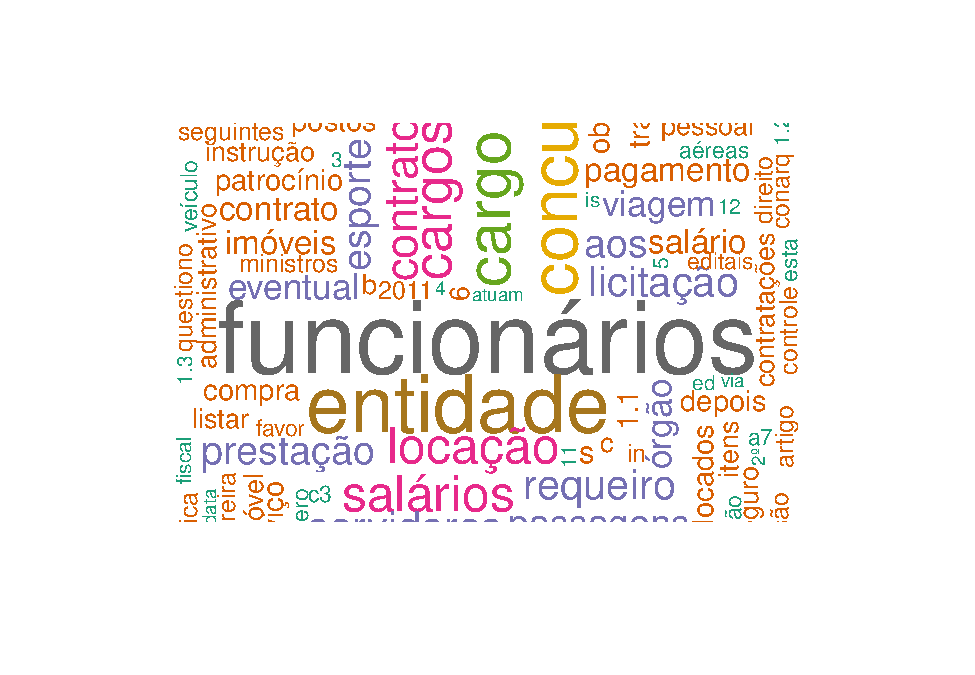
\includegraphics{markdown_v21_files/figure-latex/unnamed-chunk-39-2.pdf}

\begin{Shaded}
\begin{Highlighting}[]
\NormalTok{## DEA}
\CommentTok{#jpeg("XX_wordclou_tfidf_dir03_DEA.jpeg")}
\NormalTok{nuvem3 =}\StringTok{ }
\NormalTok{plot_diretorias_tf_dif }\OperatorTok
\StringTok{  }\KeywordTok{filter}\NormalTok{(DIRETORIA }\OperatorTok{==}\StringTok{ "DEA"}\NormalTok{) }\OperatorTok
\StringTok{  }\KeywordTok{select}\NormalTok{(}\OperatorTok{-}\NormalTok{DIRETORIA, }\DataTypeTok{word =}\NormalTok{ palavra,}\DataTypeTok{freq =}\NormalTok{ tf_idf) }\OperatorTok
\StringTok{  }\CommentTok{#top_n(150, freq) %>%}
\StringTok{  }\KeywordTok{as.data.frame}\NormalTok{() }

\KeywordTok{set.seed}\NormalTok{(}\DecValTok{231321}\NormalTok{)}
\KeywordTok{wordcloud}\NormalTok{(}\DataTypeTok{words =}\NormalTok{ nuvem3}\OperatorTok{$}\NormalTok{word, }\DataTypeTok{freq =}\NormalTok{ nuvem3}\OperatorTok{$}\NormalTok{freq, }\DataTypeTok{min.freq =} \FloatTok{0.2}\NormalTok{,}
          \DataTypeTok{max.words=}\DecValTok{250}\NormalTok{, }\DataTypeTok{random.order=}\OtherTok{FALSE}\NormalTok{, }\DataTypeTok{rot.per=}\FloatTok{0.35}\NormalTok{, }
          \DataTypeTok{colors=}\KeywordTok{brewer.pal}\NormalTok{(}\DecValTok{10}\NormalTok{, }\StringTok{"Dark2"}\NormalTok{))}
\end{Highlighting}
\end{Shaded}

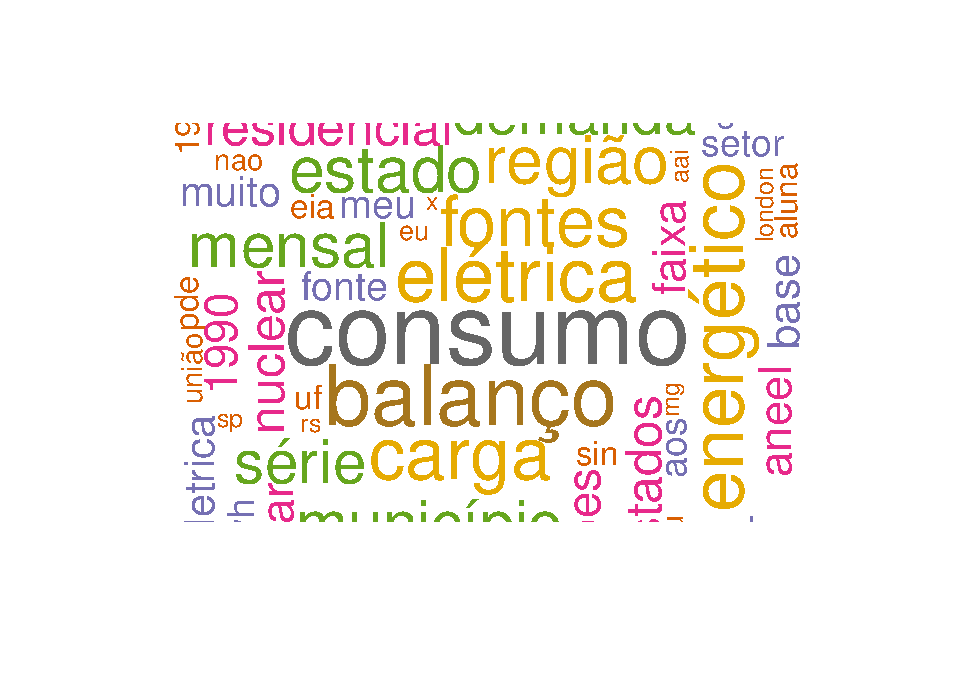
\includegraphics{markdown_v21_files/figure-latex/unnamed-chunk-39-3.pdf}

\begin{Shaded}
\begin{Highlighting}[]
\NormalTok{## DPG}
\CommentTok{#jpeg("XX_wordclou_tfidf_dir04_DPG.jpeg")}
\NormalTok{nuvem4 =}\StringTok{ }
\NormalTok{plot_diretorias_tf_dif }\OperatorTok
\StringTok{  }\KeywordTok{filter}\NormalTok{(DIRETORIA }\OperatorTok{==}\StringTok{ "DPG"}\NormalTok{) }\OperatorTok
\StringTok{  }\KeywordTok{select}\NormalTok{(}\OperatorTok{-}\NormalTok{DIRETORIA, }\DataTypeTok{word =}\NormalTok{ palavra,}\DataTypeTok{freq =}\NormalTok{ tf_idf) }\OperatorTok
\StringTok{  }\CommentTok{#top_n(150, freq) %>%}
\StringTok{  }\KeywordTok{as.data.frame}\NormalTok{() }

\KeywordTok{set.seed}\NormalTok{(}\DecValTok{75437}\NormalTok{)}
\KeywordTok{wordcloud}\NormalTok{(}\DataTypeTok{words =}\NormalTok{ nuvem4}\OperatorTok{$}\NormalTok{word, }\DataTypeTok{freq =}\NormalTok{ nuvem4}\OperatorTok{$}\NormalTok{freq, }\DataTypeTok{min.freq =} \FloatTok{0.1}\NormalTok{,}
          \DataTypeTok{max.words=}\DecValTok{250}\NormalTok{, }\DataTypeTok{random.order=}\OtherTok{FALSE}\NormalTok{, }\DataTypeTok{rot.per=}\FloatTok{0.35}\NormalTok{, }
          \DataTypeTok{colors=}\KeywordTok{brewer.pal}\NormalTok{(}\DecValTok{10}\NormalTok{, }\StringTok{"Dark2"}\NormalTok{))}
\end{Highlighting}
\end{Shaded}

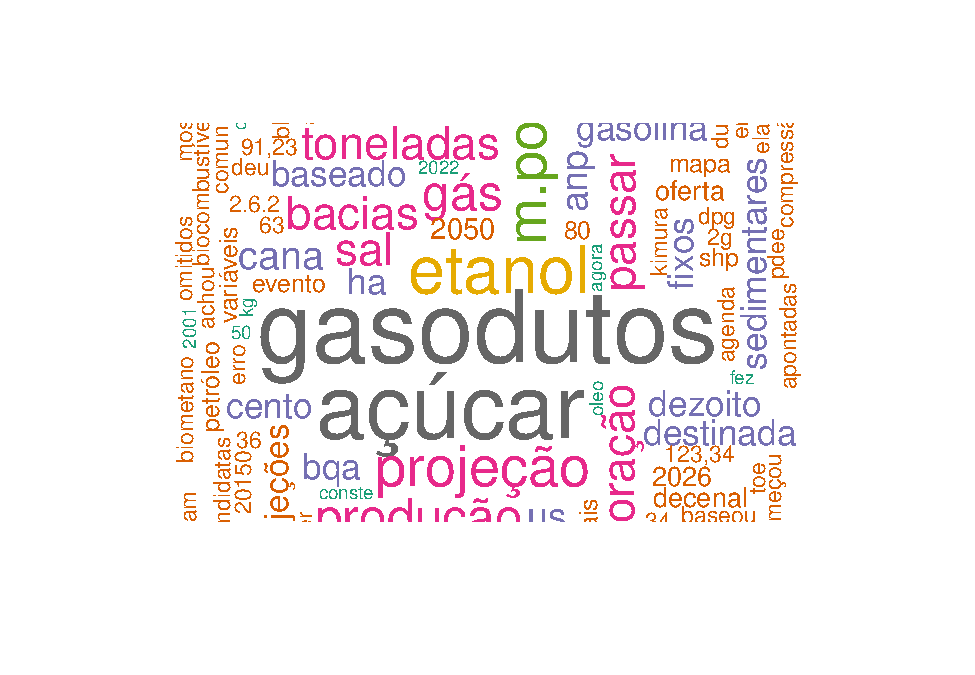
\includegraphics{markdown_v21_files/figure-latex/unnamed-chunk-39-4.pdf}

\begin{Shaded}
\begin{Highlighting}[]
\NormalTok{## OUTROS}
\CommentTok{#jpeg("XX_wordclou_tfidf_dir05_OUTROS.jpeg")}
\NormalTok{nuvem5 =}\StringTok{ }
\NormalTok{plot_diretorias_tf_dif }\OperatorTok
\StringTok{  }\KeywordTok{filter}\NormalTok{(DIRETORIA }\OperatorTok{==}\StringTok{ "OUTROS"}\NormalTok{) }\OperatorTok
\StringTok{  }\KeywordTok{select}\NormalTok{(}\OperatorTok{-}\NormalTok{DIRETORIA, }\DataTypeTok{word =}\NormalTok{ palavra,}\DataTypeTok{freq =}\NormalTok{ tf_idf) }\OperatorTok
\StringTok{  }\CommentTok{#top_n(150, freq) %>%}
\StringTok{  }\KeywordTok{as.data.frame}\NormalTok{() }

\KeywordTok{set.seed}\NormalTok{(}\DecValTok{75437}\NormalTok{)}
\KeywordTok{wordcloud}\NormalTok{(}\DataTypeTok{words =}\NormalTok{ nuvem5}\OperatorTok{$}\NormalTok{word, }\DataTypeTok{freq =}\NormalTok{ nuvem5}\OperatorTok{$}\NormalTok{freq, }\DataTypeTok{min.freq =} \FloatTok{0.1}\NormalTok{,}
          \DataTypeTok{max.words=}\DecValTok{250}\NormalTok{, }\DataTypeTok{random.order=}\OtherTok{FALSE}\NormalTok{, }\DataTypeTok{rot.per=}\FloatTok{0.35}\NormalTok{, }
          \DataTypeTok{colors=}\KeywordTok{brewer.pal}\NormalTok{(}\DecValTok{10}\NormalTok{, }\StringTok{"Dark2"}\NormalTok{))}
\end{Highlighting}
\end{Shaded}

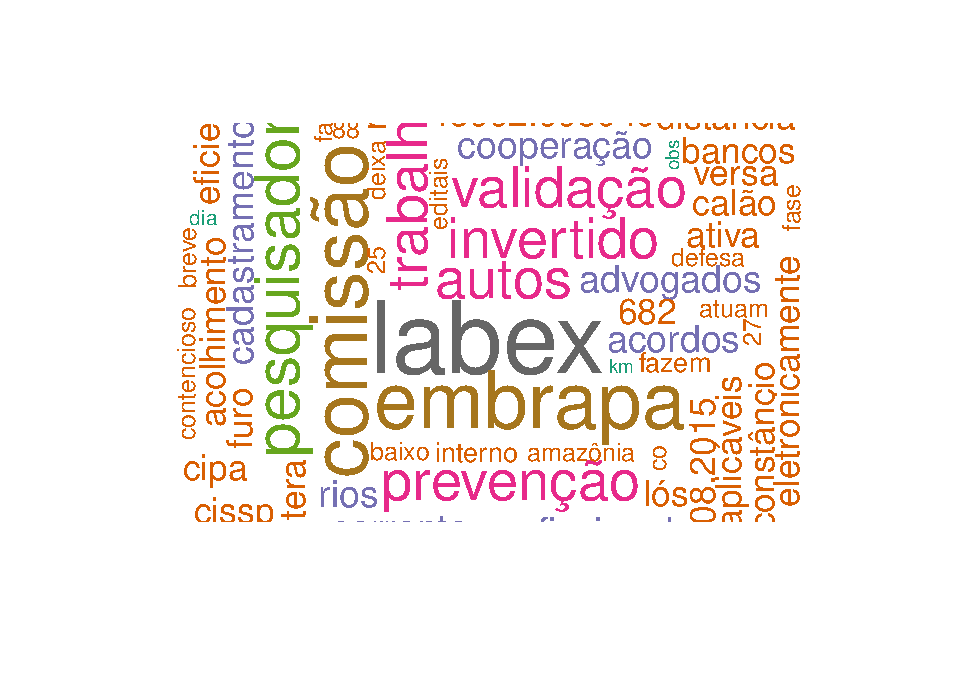
\includegraphics{markdown_v21_files/figure-latex/unnamed-chunk-39-5.pdf}

\begin{Shaded}
\begin{Highlighting}[]
\CommentTok{#View(head(plot_diretoria_palavras))}
\NormalTok{library(wordcloud2)}

\NormalTok{plot_diretorias_tf_dif = plot_diretoria_palavras %>%}
\NormalTok{    select(palavra, tf_idf, DIRETORIA) %>%}
\NormalTok{    mutate(palavra = reorder(palavra, tf_idf))}

\CommentTok{## DEE}
\CommentTok{#jpeg("XX_wordclou_tfidf_dir01_DEE.jpeg")}
\NormalTok{set.seed(233115)}
\NormalTok{plot_diretorias_tf_dif %>%}
\NormalTok{  filter(DIRETORIA == }\StringTok{"DEE"}\NormalTok{) %>%}
\NormalTok{  top_n(150, tf_idf) %>%}
\NormalTok{  wordcloud2(shuffle = TRUE, }
\NormalTok{             color = }\StringTok{"random-dark"}\NormalTok{,}
\NormalTok{             shape = }\StringTok{"circle"}\NormalTok{)}

\CommentTok{## DGC}
\CommentTok{#jpeg("XX_wordclou_tfidf_dir01_DGC.jpeg")}
\NormalTok{set.seed(233115)}
\NormalTok{plot_diretorias_tf_dif %>%}
\NormalTok{  filter(DIRETORIA == }\StringTok{"DGC"}\NormalTok{) %>%}
\NormalTok{  top_n(150, tf_idf) %>%}
\NormalTok{  wordcloud2()}

\CommentTok{## DEA}
\CommentTok{#jpeg("XX_wordclou_tfidf_dir01_DEA.jpeg")}
\NormalTok{set.seed(233115)}
\NormalTok{plot_diretorias_tf_dif %>%}
\NormalTok{  filter(DIRETORIA == }\StringTok{"DEA"}\NormalTok{) %>%}
\NormalTok{  top_n(150, tf_idf) %>%}
\NormalTok{  wordcloud2()}

\CommentTok{## DPG}
\CommentTok{#jpeg("XX_wordclou_tfidf_dir04_DPG.jpeg")}
\NormalTok{set.seed(233115)}
\NormalTok{plot_diretorias_tf_dif %>%}
\NormalTok{  filter(DIRETORIA == }\StringTok{"DPG"}\NormalTok{) %>%}
\NormalTok{  top_n(150, tf_idf) %>%}
\NormalTok{  wordcloud2()}
  
\CommentTok{## OUTROS}
\CommentTok{#jpeg("XX_wordclou_tfidf_dir01_OUTROS.jpeg")}
\NormalTok{set.seed(233115)}
\NormalTok{plot_diretorias_tf_dif %>%}
\NormalTok{  filter(DIRETORIA == }\StringTok{"OUTROS"}\NormalTok{) %>%}
\NormalTok{  top_n(150, tf_idf) %>%}
\NormalTok{  wordcloud2()}
\end{Highlighting}
\end{Shaded}

--\textgreater{}

\paragraph{Nuvem de palavras por diretoria - s/ steeming e/ou remoção de
stopwords -
bigram}\label{nuvem-de-palavras-por-diretoria---s-steeming-eou-remocao-de-stopwords---bigram}

\begin{Shaded}
\begin{Highlighting}[]
\NormalTok{plot_diretorias_tf_dif_bigram =}\StringTok{ }\NormalTok{DB }\OperatorTok
\StringTok{  }\KeywordTok{select}\NormalTok{(DESCRI_PEDIDO,DIRETORIA) }\OperatorTok
\StringTok{  }\KeywordTok{unnest_tokens}\NormalTok{(BIGRAM, DESCRI_PEDIDO, }\DataTypeTok{token =} \StringTok{"ngrams"}\NormalTok{, }\DataTypeTok{n =} \DecValTok{2}\NormalTok{) }\OperatorTok
\StringTok{  }\KeywordTok{count}\NormalTok{(DIRETORIA, BIGRAM, }\DataTypeTok{sort =} \OtherTok{TRUE}\NormalTok{) }\OperatorTok
\StringTok{  }\KeywordTok{bind_tf_idf}\NormalTok{(BIGRAM, DIRETORIA, n) }\OperatorTok
\StringTok{  }\KeywordTok{arrange}\NormalTok{(}\KeywordTok{desc}\NormalTok{(tf_idf)) }\OperatorTok
\StringTok{  }\KeywordTok{mutate}\NormalTok{(}\DataTypeTok{BIGRAM =} \KeywordTok{factor}\NormalTok{(BIGRAM, }\DataTypeTok{levels =} \KeywordTok{rev}\NormalTok{(}\KeywordTok{unique}\NormalTok{(BIGRAM)))) }\OperatorTok
\StringTok{  }\KeywordTok{mutate}\NormalTok{(}\DataTypeTok{DIRETORIA =} \KeywordTok{factor}\NormalTok{(DIRETORIA,}\DataTypeTok{levels=}\KeywordTok{c}\NormalTok{(}\StringTok{"DEA"}\NormalTok{,}\StringTok{"DEE"}\NormalTok{,}\StringTok{"DGC"}\NormalTok{,}\StringTok{"DPG"}\NormalTok{,}\StringTok{"OUTROS"}\NormalTok{))) }\OperatorTok
\StringTok{  }\KeywordTok{select}\NormalTok{(BIGRAM, tf_idf, DIRETORIA)}
\end{Highlighting}
\end{Shaded}

\begin{Shaded}
\begin{Highlighting}[]
\NormalTok{## DEE}
\CommentTok{#jpeg("XX_wordclou_tfidf_dir01_DEE.jpeg")}
\NormalTok{nuvem1.}\DecValTok{2}\NormalTok{ =}\StringTok{ }
\NormalTok{plot_diretorias_tf_dif_bigram }\OperatorTok
\StringTok{  }\KeywordTok{filter}\NormalTok{(DIRETORIA }\OperatorTok{==}\StringTok{ "DEE"}\NormalTok{) }\OperatorTok
\StringTok{  }\KeywordTok{select}\NormalTok{(}\OperatorTok{-}\NormalTok{DIRETORIA, }\DataTypeTok{word =}\NormalTok{ BIGRAM,}\DataTypeTok{freq =}\NormalTok{ tf_idf) }\OperatorTok
\StringTok{  }\CommentTok{#top_n(150, freq) %>%}
\StringTok{  }\KeywordTok{as.data.frame}\NormalTok{() }

\KeywordTok{set.seed}\NormalTok{(}\DecValTok{231321}\NormalTok{)}
\KeywordTok{wordcloud}\NormalTok{(}\DataTypeTok{words =}\NormalTok{ nuvem1.}\DecValTok{2}\OperatorTok{$}\NormalTok{word, }\DataTypeTok{freq =}\NormalTok{ nuvem1.}\DecValTok{2}\OperatorTok{$}\NormalTok{freq, }\DataTypeTok{min.freq =} \FloatTok{0.2}\NormalTok{,}
          \DataTypeTok{max.words=}\DecValTok{250}\NormalTok{, }\DataTypeTok{random.order=}\OtherTok{FALSE}\NormalTok{, }\DataTypeTok{rot.per=}\FloatTok{0.35}\NormalTok{, }
          \DataTypeTok{colors=}\KeywordTok{brewer.pal}\NormalTok{(}\DecValTok{10}\NormalTok{, }\StringTok{"Dark2"}\NormalTok{))}
\end{Highlighting}
\end{Shaded}

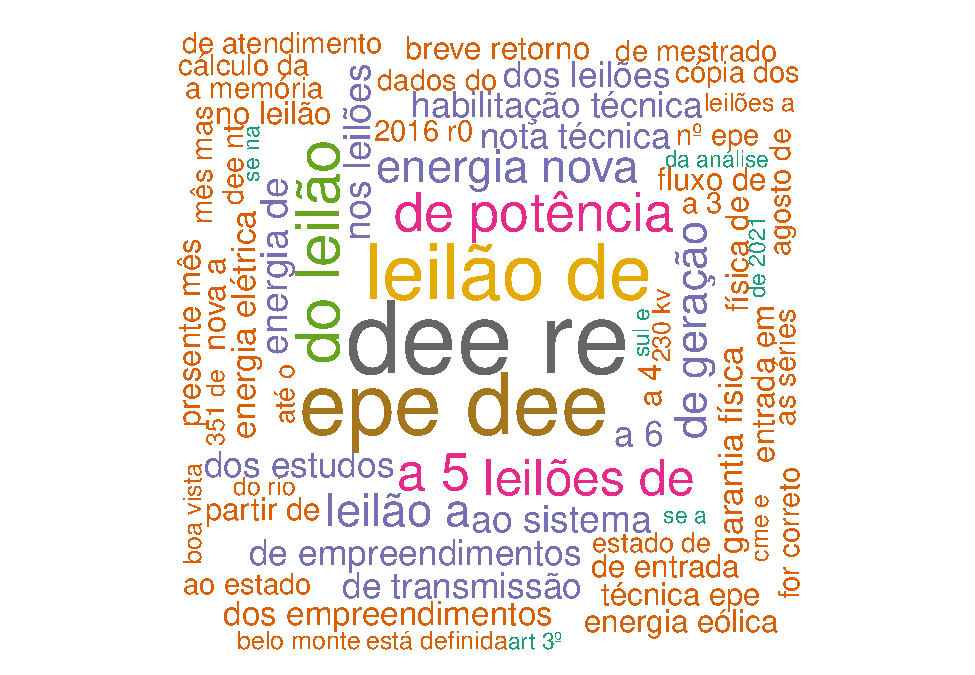
\includegraphics{markdown_v21_files/figure-latex/wordcloud_onegram_DIR01_semstopwords-1.pdf}

\begin{Shaded}
\begin{Highlighting}[]
\NormalTok{## DGC}
\CommentTok{#jpeg("XX_wordclou_tfidf_dir02_DGC.jpeg")}
\NormalTok{nuvem2.}\DecValTok{2}\NormalTok{ =}\StringTok{ }
\NormalTok{plot_diretorias_tf_dif_bigram }\OperatorTok
\StringTok{  }\KeywordTok{filter}\NormalTok{(DIRETORIA }\OperatorTok{==}\StringTok{ "DGC"}\NormalTok{) }\OperatorTok
\StringTok{  }\KeywordTok{select}\NormalTok{(}\OperatorTok{-}\NormalTok{DIRETORIA, }\DataTypeTok{word =}\NormalTok{ BIGRAM,}\DataTypeTok{freq =}\NormalTok{ tf_idf) }\OperatorTok
\StringTok{  }\CommentTok{#top_n(150, freq) %>%}
\StringTok{  }\KeywordTok{as.data.frame}\NormalTok{() }

\KeywordTok{set.seed}\NormalTok{(}\DecValTok{75437}\NormalTok{)}
\KeywordTok{wordcloud}\NormalTok{(}\DataTypeTok{words =}\NormalTok{ nuvem2.}\DecValTok{2}\OperatorTok{$}\NormalTok{word, }\DataTypeTok{freq =}\NormalTok{ nuvem2.}\DecValTok{2}\OperatorTok{$}\NormalTok{freq, }\DataTypeTok{min.freq =} \FloatTok{0.2}\NormalTok{,}
          \DataTypeTok{max.words=}\DecValTok{250}\NormalTok{, }\DataTypeTok{random.order=}\OtherTok{FALSE}\NormalTok{, }\DataTypeTok{rot.per=}\FloatTok{0.35}\NormalTok{, }
          \DataTypeTok{colors=}\KeywordTok{brewer.pal}\NormalTok{(}\DecValTok{10}\NormalTok{, }\StringTok{"Dark2"}\NormalTok{))}
\end{Highlighting}
\end{Shaded}

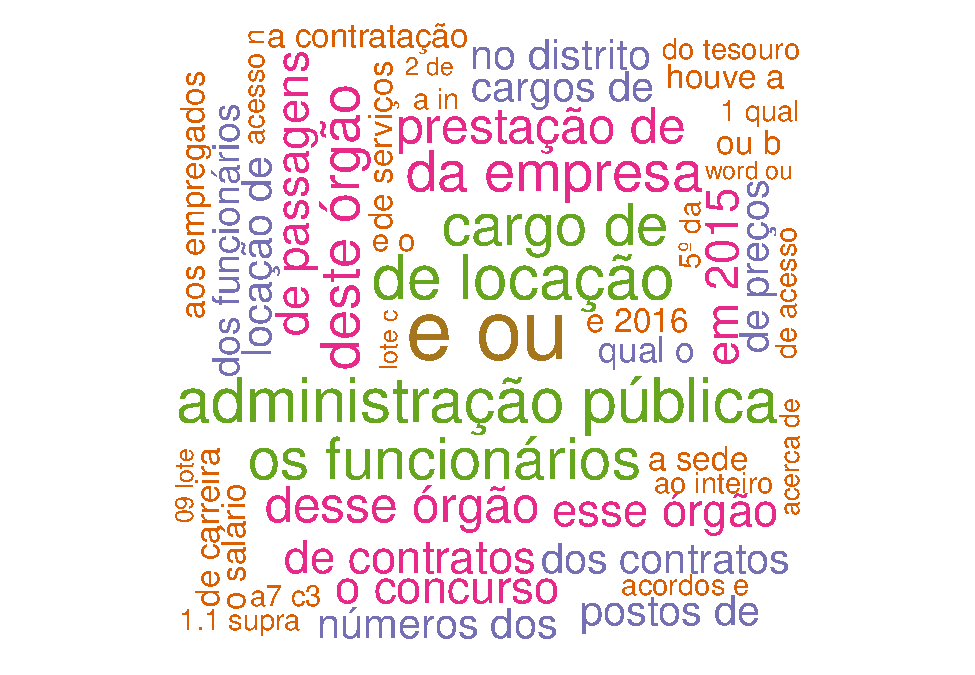
\includegraphics{markdown_v21_files/figure-latex/wordcloud_onegram_DIR02_semstopwords-1.pdf}

\begin{Shaded}
\begin{Highlighting}[]
\NormalTok{## DEA}
\CommentTok{#jpeg("XX_wordclou_tfidf_dir03_DEA.jpeg")}
\NormalTok{nuvem3.}\DecValTok{2}\NormalTok{ =}\StringTok{ }
\NormalTok{plot_diretorias_tf_dif_bigram }\OperatorTok
\StringTok{  }\KeywordTok{filter}\NormalTok{(DIRETORIA }\OperatorTok{==}\StringTok{ "DEA"}\NormalTok{) }\OperatorTok
\StringTok{  }\KeywordTok{select}\NormalTok{(}\OperatorTok{-}\NormalTok{DIRETORIA, }\DataTypeTok{word =}\NormalTok{ BIGRAM,}\DataTypeTok{freq =}\NormalTok{ tf_idf) }\OperatorTok
\StringTok{  }\CommentTok{#top_n(150, freq) %>%}
\StringTok{  }\KeywordTok{as.data.frame}\NormalTok{() }

\KeywordTok{set.seed}\NormalTok{(}\DecValTok{543453}\NormalTok{)}
\KeywordTok{wordcloud}\NormalTok{(}\DataTypeTok{words =}\NormalTok{ nuvem3.}\DecValTok{2}\OperatorTok{$}\NormalTok{word, }\DataTypeTok{freq =}\NormalTok{ nuvem3.}\DecValTok{2}\OperatorTok{$}\NormalTok{freq, }\DataTypeTok{min.freq =} \FloatTok{0.2}\NormalTok{,}
          \DataTypeTok{max.words=}\DecValTok{250}\NormalTok{, }\DataTypeTok{random.order=}\OtherTok{FALSE}\NormalTok{, }\DataTypeTok{rot.per=}\FloatTok{0.35}\NormalTok{, }
          \DataTypeTok{colors=}\KeywordTok{brewer.pal}\NormalTok{(}\DecValTok{10}\NormalTok{, }\StringTok{"Dark2"}\NormalTok{))}
\end{Highlighting}
\end{Shaded}

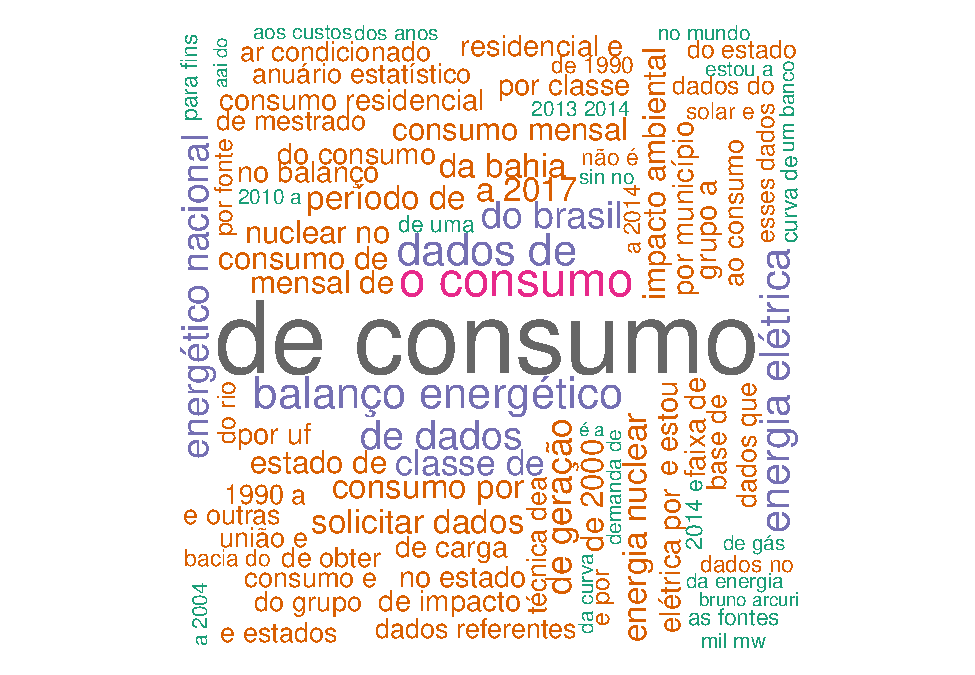
\includegraphics{markdown_v21_files/figure-latex/wordcloud_onegram_DIR03_semstopwords-1.pdf}

\begin{Shaded}
\begin{Highlighting}[]
\NormalTok{## DPG}
\CommentTok{#jpeg("XX_wordclou_tfidf_dir04_DPG.jpeg")}
\NormalTok{nuvem4.}\DecValTok{2}\NormalTok{ =}\StringTok{ }
\NormalTok{plot_diretorias_tf_dif_bigram }\OperatorTok
\StringTok{  }\KeywordTok{filter}\NormalTok{(DIRETORIA }\OperatorTok{==}\StringTok{ "DPG"}\NormalTok{) }\OperatorTok
\StringTok{  }\KeywordTok{select}\NormalTok{(}\OperatorTok{-}\NormalTok{DIRETORIA, }\DataTypeTok{word =}\NormalTok{ BIGRAM,}\DataTypeTok{freq =}\NormalTok{ tf_idf) }\OperatorTok
\StringTok{  }\CommentTok{#top_n(150, freq) %>%}
\StringTok{  }\KeywordTok{as.data.frame}\NormalTok{() }

\KeywordTok{set.seed}\NormalTok{(}\DecValTok{75437}\NormalTok{)}
\KeywordTok{wordcloud}\NormalTok{(}\DataTypeTok{words =}\NormalTok{ nuvem4.}\DecValTok{2}\OperatorTok{$}\NormalTok{word, }\DataTypeTok{freq =}\NormalTok{ nuvem4.}\DecValTok{2}\OperatorTok{$}\NormalTok{freq, }\DataTypeTok{min.freq =} \FloatTok{0.1}\NormalTok{,}
          \DataTypeTok{max.words=}\DecValTok{250}\NormalTok{, }\DataTypeTok{random.order=}\OtherTok{FALSE}\NormalTok{, }\DataTypeTok{rot.per=}\FloatTok{0.35}\NormalTok{, }
          \DataTypeTok{colors=}\KeywordTok{brewer.pal}\NormalTok{(}\DecValTok{10}\NormalTok{, }\StringTok{"Dark2"}\NormalTok{))}
\end{Highlighting}
\end{Shaded}

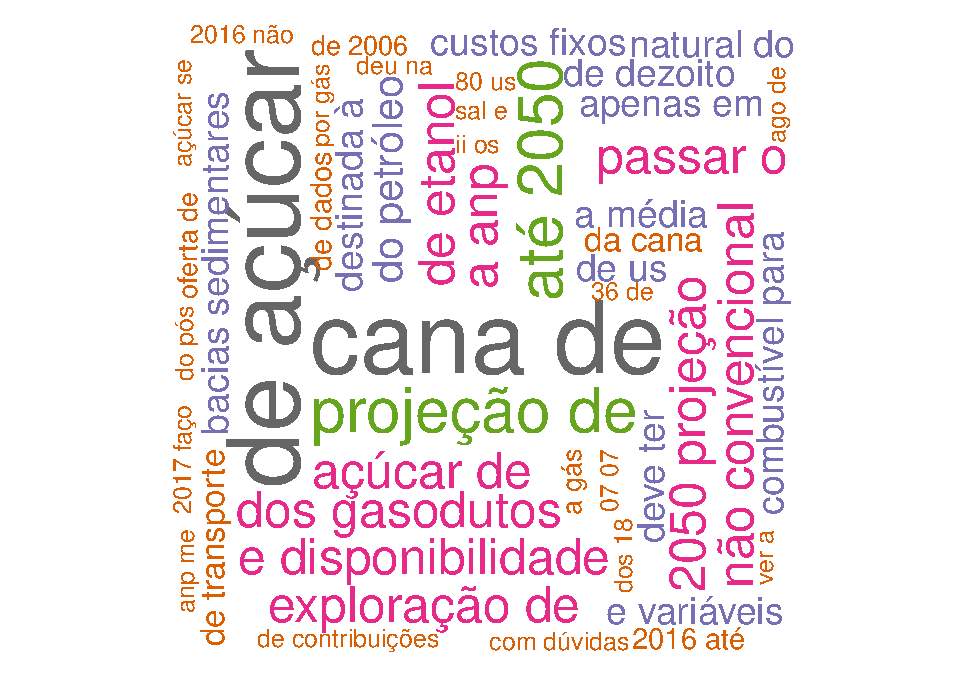
\includegraphics{markdown_v21_files/figure-latex/wordcloud_onegram_DIR04_semstopwords-1.pdf}

\begin{Shaded}
\begin{Highlighting}[]
\NormalTok{## OUTROS}
\CommentTok{#jpeg("XX_wordclou_tfidf_dir05_OUTROS.jpeg")}
\NormalTok{nuvem5.}\DecValTok{2}\NormalTok{ =}\StringTok{ }
\NormalTok{plot_diretorias_tf_dif_bigram }\OperatorTok
\StringTok{  }\KeywordTok{filter}\NormalTok{(DIRETORIA }\OperatorTok{==}\StringTok{ "OUTROS"}\NormalTok{) }\OperatorTok
\StringTok{  }\KeywordTok{select}\NormalTok{(}\OperatorTok{-}\NormalTok{DIRETORIA, }\DataTypeTok{word =}\NormalTok{ BIGRAM,}\DataTypeTok{freq =}\NormalTok{ tf_idf) }\OperatorTok
\StringTok{  }\CommentTok{#top_n(150, freq) %>%}
\StringTok{  }\KeywordTok{as.data.frame}\NormalTok{() }

\KeywordTok{set.seed}\NormalTok{(}\DecValTok{75437}\NormalTok{)}
\KeywordTok{wordcloud}\NormalTok{(}\DataTypeTok{words =}\NormalTok{ nuvem5.}\DecValTok{2}\OperatorTok{$}\NormalTok{word, }\DataTypeTok{freq =}\NormalTok{ nuvem5.}\DecValTok{2}\OperatorTok{$}\NormalTok{freq, }\DataTypeTok{min.freq =} \FloatTok{0.1}\NormalTok{,}
          \DataTypeTok{max.words=}\DecValTok{250}\NormalTok{, }\DataTypeTok{random.order=}\OtherTok{FALSE}\NormalTok{, }\DataTypeTok{rot.per=}\FloatTok{0.35}\NormalTok{, }
          \DataTypeTok{colors=}\KeywordTok{brewer.pal}\NormalTok{(}\DecValTok{10}\NormalTok{, }\StringTok{"Dark2"}\NormalTok{))}
\end{Highlighting}
\end{Shaded}

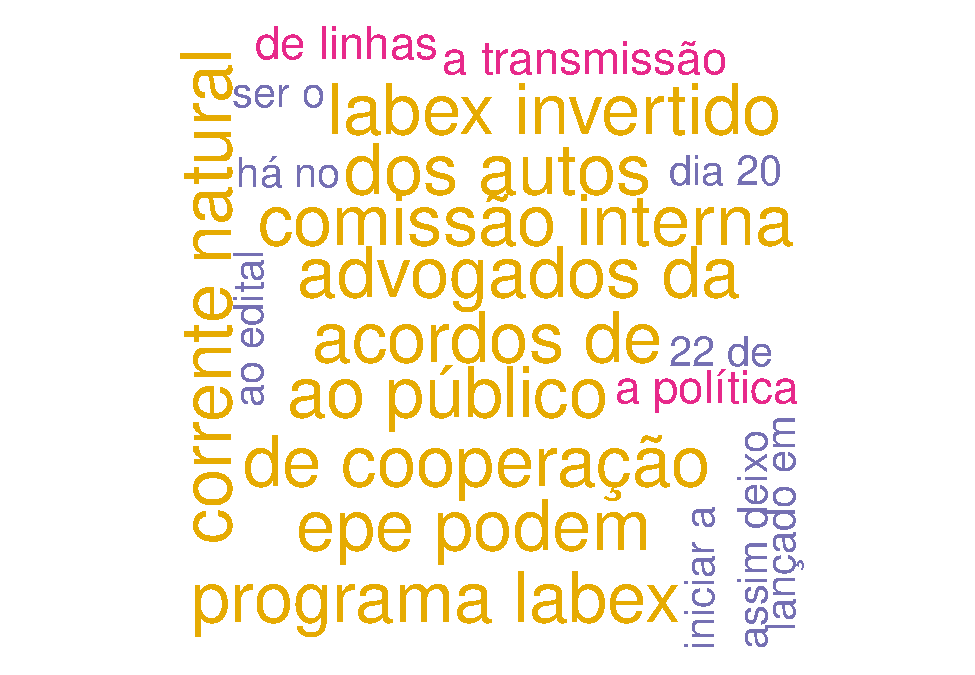
\includegraphics{markdown_v21_files/figure-latex/wordcloud_onegram_DIR05_semstopwords-1.pdf}

\begin{Shaded}
\begin{Highlighting}[]
\CommentTok{#View(head(plot_diretoria_palavras))}
\NormalTok{library(wordcloud2)}

\NormalTok{plot_diretorias_tf_dif_bigram = DB %>%}
\NormalTok{  select(DESCRI_PEDIDO,DIRETORIA) %>%}
\NormalTok{  unnest_tokens(BIGRAM, DESCRI_PEDIDO, token = }\StringTok{"ngrams"}\NormalTok{, n = 2) %>%}
\NormalTok{  count(DIRETORIA, BIGRAM, sort = TRUE) %>%}
\NormalTok{  bind_tf_idf(BIGRAM, DIRETORIA, n) %>%}
\NormalTok{  arrange(desc(tf_idf)) %>%}
\NormalTok{  mutate(BIGRAM = factor(BIGRAM, levels = rev(unique(BIGRAM)))) %>%}
\NormalTok{  mutate(DIRETORIA = factor(DIRETORIA,levels=c(}\StringTok{"DEA"}\NormalTok{,}\StringTok{"DEE"}\NormalTok{,}\StringTok{"DGC"}\NormalTok{,}\StringTok{"DPG"}\NormalTok{,}\StringTok{"OUTROS"}\NormalTok{))) %>%}
\NormalTok{  select(BIGRAM, tf_idf, DIRETORIA)}
  

\CommentTok{## DEE}
\CommentTok{#jpeg("XX_wordclou_tfidf_dir01_DEE.jpeg")}
\NormalTok{set.seed(233115)}
\NormalTok{plot_diretorias_tf_dif_bigram %>%}
\NormalTok{  filter(DIRETORIA == }\StringTok{"DEE"}\NormalTok{) %>%}
\NormalTok{  top_n(150, tf_idf) %>%}
\NormalTok{  wordcloud2(shuffle = TRUE, }
\NormalTok{             color = }\StringTok{"random-dark"}\NormalTok{,}
\NormalTok{             shape = }\StringTok{"circle"}\NormalTok{)}

\CommentTok{## DGC}
\CommentTok{#jpeg("XX_wordclou_tfidf_dir01_DGC.jpeg")}
\NormalTok{set.seed(233115)}
\NormalTok{plot_diretorias_tf_dif_bigram %>%}
\NormalTok{  filter(DIRETORIA == }\StringTok{"DGC"}\NormalTok{) %>%}
\NormalTok{  top_n(150, tf_idf) %>%}
\NormalTok{  wordcloud2()}

\CommentTok{## DEA}
\CommentTok{#jpeg("XX_wordclou_tfidf_dir01_DEA.jpeg")}
\NormalTok{set.seed(233115)}
\NormalTok{plot_diretorias_tf_dif_bigram %>%}
\NormalTok{  filter(DIRETORIA == }\StringTok{"DEA"}\NormalTok{) %>%}
\NormalTok{  top_n(150, tf_idf) %>%}
\NormalTok{  wordcloud2()}

\CommentTok{## DPG}
\CommentTok{#jpeg("XX_wordclou_tfidf_dir01_DPG.jpeg")}
\NormalTok{set.seed(233115)}
\NormalTok{plot_diretorias_tf_dif_bigram %>%}
\NormalTok{  filter(DIRETORIA == }\StringTok{"DPG"}\NormalTok{) %>%}
\NormalTok{  top_n(150, tf_idf) %>%}
\NormalTok{  wordcloud2()}
\end{Highlighting}
\end{Shaded}

\subparagraph{\texorpdfstring{Separando palavras de um bigram em
``palavra1'' e ``palavra2'' p/ remover
stopwords}{Separando palavras de um bigram em palavra1 e palavra2 p/ remover stopwords}}\label{separando-palavras-de-um-bigram-em-palavra1-e-palavra2-p-remover-stopwords}

Considerando já a exclusão de casos onde houver stopwords consecultivos
na ``palavra1'' e ``palavra2'', ou seja onde
\(palavra1=stopword \land palavra2=stopword\)

\begin{Shaded}
\begin{Highlighting}[]
\NormalTok{bigrams =}\StringTok{ }\NormalTok{DB }\OperatorTok
\StringTok{  }\KeywordTok{select}\NormalTok{(DESCRI_PEDIDO,DIRETORIA) }\OperatorTok
\StringTok{  }\KeywordTok{unnest_tokens}\NormalTok{(BIGRAM, DESCRI_PEDIDO, }\DataTypeTok{token =} \StringTok{"ngrams"}\NormalTok{, }\DataTypeTok{n =} \DecValTok{2}\NormalTok{) }\OperatorTok
\StringTok{  }\KeywordTok{count}\NormalTok{(DIRETORIA, BIGRAM, }\DataTypeTok{sort =} \OtherTok{TRUE}\NormalTok{) }

\NormalTok{separa_bigrams =}\StringTok{ }\NormalTok{bigrams }\OperatorTok
\StringTok{  }\KeywordTok{separate}\NormalTok{(BIGRAM, }\KeywordTok{c}\NormalTok{(}\StringTok{"palavra1"}\NormalTok{, }\StringTok{"palavra2"}\NormalTok{), }\DataTypeTok{sep =} \StringTok{" "}\NormalTok{)}

\NormalTok{junta_bigrams =}\StringTok{ }\NormalTok{separa_bigrams }\OperatorTok
\StringTok{  }\KeywordTok{unite}\NormalTok{(BIGRAM, palavra1, palavra2, }\DataTypeTok{sep =} \StringTok{" "}\NormalTok{)}
\CommentTok{# levels(as.factor(junta_bigrams$BIGRAM == bigrams$BIGRAM))   # CHECK}

\NormalTok{## remove stopwords  }
\NormalTok{bigrams2 =}\StringTok{ }\KeywordTok{cbind}\NormalTok{(separa_bigrams,}\DataTypeTok{BIGRAM =}\NormalTok{ junta_bigrams}\OperatorTok{$}\NormalTok{BIGRAM) }\OperatorTok
\StringTok{  }\KeywordTok{filter}\NormalTok{(}\OperatorTok{!}\NormalTok{palavra1 }\OperatorTok\StringTok{ }\NormalTok{mystopwords}\OperatorTok{$}\NormalTok{palavra) }\OperatorTok
\StringTok{  }\KeywordTok{filter}\NormalTok{(}\OperatorTok{!}\NormalTok{palavra2 }\OperatorTok\StringTok{ }\NormalTok{mystopwords}\OperatorTok{$}\NormalTok{palavra) }\OperatorTok\StringTok{  }
\StringTok{  }\KeywordTok{filter}\NormalTok{(}\OperatorTok{!}\NormalTok{palavra1 }\OperatorTok\StringTok{ "a"}\NormalTok{) }\OperatorTok
\StringTok{  }\KeywordTok{filter}\NormalTok{(}\OperatorTok{!}\NormalTok{palavra2 }\OperatorTok\StringTok{ "a"}\NormalTok{) }\OperatorTok
\StringTok{  }\KeywordTok{filter}\NormalTok{(}\OperatorTok{!}\NormalTok{palavra1 }\OperatorTok\StringTok{ "p"}\NormalTok{) }\OperatorTok
\StringTok{  }\KeywordTok{filter}\NormalTok{(}\OperatorTok{!}\NormalTok{palavra1 }\OperatorTok\StringTok{ "s"}\NormalTok{) }\OperatorTok
\StringTok{  }\KeywordTok{filter}\NormalTok{(}\OperatorTok{!}\NormalTok{palavra1 }\OperatorTok\StringTok{ "d"}\NormalTok{) }\OperatorTok
\StringTok{  }\KeywordTok{filter}\NormalTok{(}\OperatorTok{!}\NormalTok{palavra2 }\OperatorTok\StringTok{ "p"}\NormalTok{) }\OperatorTok
\StringTok{  }\KeywordTok{filter}\NormalTok{(}\OperatorTok{!}\NormalTok{palavra2 }\OperatorTok\StringTok{ "s"}\NormalTok{) }\OperatorTok
\StringTok{  }\KeywordTok{filter}\NormalTok{(}\OperatorTok{!}\NormalTok{palavra2 }\OperatorTok\StringTok{ "d"}\NormalTok{) }\OperatorTok
\StringTok{  }\KeywordTok{filter}\NormalTok{(}\OperatorTok{!}\NormalTok{palavra2 }\OperatorTok\StringTok{ "s.a"}\NormalTok{) }\OperatorTok
\StringTok{  }\KeywordTok{filter}\NormalTok{(}\OperatorTok{!}\KeywordTok{str_detect}\NormalTok{(palavra1, }\StringTok{"0"}\NormalTok{)) }\OperatorTok
\StringTok{  }\KeywordTok{filter}\NormalTok{(}\OperatorTok{!}\KeywordTok{str_detect}\NormalTok{(palavra1, }\StringTok{"1"}\NormalTok{)) }\OperatorTok
\StringTok{  }\KeywordTok{filter}\NormalTok{(}\OperatorTok{!}\KeywordTok{str_detect}\NormalTok{(palavra1, }\StringTok{"2"}\NormalTok{)) }\OperatorTok
\StringTok{  }\KeywordTok{filter}\NormalTok{(}\OperatorTok{!}\KeywordTok{str_detect}\NormalTok{(palavra1, }\StringTok{"3"}\NormalTok{)) }\OperatorTok
\StringTok{  }\KeywordTok{filter}\NormalTok{(}\OperatorTok{!}\KeywordTok{str_detect}\NormalTok{(palavra1, }\StringTok{"4"}\NormalTok{)) }\OperatorTok
\StringTok{  }\KeywordTok{filter}\NormalTok{(}\OperatorTok{!}\KeywordTok{str_detect}\NormalTok{(palavra1, }\StringTok{"5"}\NormalTok{)) }\OperatorTok
\StringTok{  }\KeywordTok{filter}\NormalTok{(}\OperatorTok{!}\KeywordTok{str_detect}\NormalTok{(palavra1, }\StringTok{"6"}\NormalTok{)) }\OperatorTok
\StringTok{  }\KeywordTok{filter}\NormalTok{(}\OperatorTok{!}\KeywordTok{str_detect}\NormalTok{(palavra1, }\StringTok{"7"}\NormalTok{)) }\OperatorTok
\StringTok{  }\KeywordTok{filter}\NormalTok{(}\OperatorTok{!}\KeywordTok{str_detect}\NormalTok{(palavra1, }\StringTok{"8"}\NormalTok{)) }\OperatorTok
\StringTok{  }\KeywordTok{filter}\NormalTok{(}\OperatorTok{!}\KeywordTok{str_detect}\NormalTok{(palavra1, }\StringTok{"9"}\NormalTok{)) }\OperatorTok
\StringTok{  }\KeywordTok{filter}\NormalTok{(}\OperatorTok{!}\KeywordTok{str_detect}\NormalTok{(palavra2, }\StringTok{"0"}\NormalTok{)) }\OperatorTok
\StringTok{  }\KeywordTok{filter}\NormalTok{(}\OperatorTok{!}\KeywordTok{str_detect}\NormalTok{(palavra2, }\StringTok{"1"}\NormalTok{)) }\OperatorTok
\StringTok{  }\KeywordTok{filter}\NormalTok{(}\OperatorTok{!}\KeywordTok{str_detect}\NormalTok{(palavra2, }\StringTok{"2"}\NormalTok{)) }\OperatorTok
\StringTok{  }\KeywordTok{filter}\NormalTok{(}\OperatorTok{!}\KeywordTok{str_detect}\NormalTok{(palavra2, }\StringTok{"3"}\NormalTok{)) }\OperatorTok
\StringTok{  }\KeywordTok{filter}\NormalTok{(}\OperatorTok{!}\KeywordTok{str_detect}\NormalTok{(palavra2, }\StringTok{"4"}\NormalTok{)) }\OperatorTok
\StringTok{  }\KeywordTok{filter}\NormalTok{(}\OperatorTok{!}\KeywordTok{str_detect}\NormalTok{(palavra2, }\StringTok{"5"}\NormalTok{)) }\OperatorTok
\StringTok{  }\KeywordTok{filter}\NormalTok{(}\OperatorTok{!}\KeywordTok{str_detect}\NormalTok{(palavra2, }\StringTok{"6"}\NormalTok{)) }\OperatorTok
\StringTok{  }\KeywordTok{filter}\NormalTok{(}\OperatorTok{!}\KeywordTok{str_detect}\NormalTok{(palavra2, }\StringTok{"7"}\NormalTok{)) }\OperatorTok
\StringTok{  }\KeywordTok{filter}\NormalTok{(}\OperatorTok{!}\KeywordTok{str_detect}\NormalTok{(palavra2, }\StringTok{"8"}\NormalTok{)) }\OperatorTok
\StringTok{  }\KeywordTok{filter}\NormalTok{(}\OperatorTok{!}\KeywordTok{str_detect}\NormalTok{(palavra2, }\StringTok{"9"}\NormalTok{))}
  \CommentTok{#count(DIRETORIA, BIGRAM) }
\end{Highlighting}
\end{Shaded}

\paragraph{Nuvem de palavras por diretoria - s/ steeming c/ remoção de
stopwords -
bigram}\label{nuvem-de-palavras-por-diretoria---s-steeming-c-remocao-de-stopwords---bigram}

\begin{Shaded}
\begin{Highlighting}[]
\CommentTok{#View(head(plot_diretoria_palavras))}
\KeywordTok{library}\NormalTok{(wordcloud2)}
\KeywordTok{library}\NormalTok{(wordcloud)}
\NormalTok{plot_diretorias_tf_dif_bigram2 =}\StringTok{ }\NormalTok{bigrams2 }\OperatorTok
\StringTok{  }\KeywordTok{select}\NormalTok{(BIGRAM,n,DIRETORIA) }\OperatorTok
\StringTok{  }\KeywordTok{bind_tf_idf}\NormalTok{(BIGRAM, DIRETORIA, n) }\OperatorTok
\StringTok{  }\KeywordTok{arrange}\NormalTok{(}\KeywordTok{desc}\NormalTok{(tf_idf)) }\OperatorTok
\StringTok{  }\KeywordTok{mutate}\NormalTok{(}\DataTypeTok{BIGRAM =} \KeywordTok{factor}\NormalTok{(BIGRAM, }\DataTypeTok{levels =} \KeywordTok{rev}\NormalTok{(}\KeywordTok{unique}\NormalTok{(BIGRAM)))) }\OperatorTok
\StringTok{  }\KeywordTok{mutate}\NormalTok{(}\DataTypeTok{DIRETORIA =} \KeywordTok{factor}\NormalTok{(DIRETORIA,}\DataTypeTok{levels=}\KeywordTok{c}\NormalTok{(}\StringTok{"DEA"}\NormalTok{,}\StringTok{"DEE"}\NormalTok{,}\StringTok{"DGC"}\NormalTok{,}\StringTok{"DPG"}\NormalTok{,}\StringTok{"OUTROS"}\NormalTok{))) }\OperatorTok
\StringTok{  }\KeywordTok{select}\NormalTok{(BIGRAM, tf_idf, DIRETORIA)}
\end{Highlighting}
\end{Shaded}

\begin{Shaded}
\begin{Highlighting}[]
\NormalTok{## DEE}
\CommentTok{#jpeg("XX_wordclou_tfidf_dir01_DEE.jpeg")}
\NormalTok{nuvem1.}\DecValTok{2}\NormalTok{ =}\StringTok{ }
\NormalTok{plot_diretorias_tf_dif_bigram2 }\OperatorTok
\StringTok{  }\KeywordTok{filter}\NormalTok{(DIRETORIA }\OperatorTok{==}\StringTok{ "DEE"}\NormalTok{) }\OperatorTok
\StringTok{  }\KeywordTok{select}\NormalTok{(}\OperatorTok{-}\NormalTok{DIRETORIA, }\DataTypeTok{word =}\NormalTok{ BIGRAM,}\DataTypeTok{freq =}\NormalTok{ tf_idf) }\OperatorTok
\StringTok{  }\CommentTok{#top_n(150, freq) %>%}
\StringTok{  }\KeywordTok{as.data.frame}\NormalTok{() }

\KeywordTok{set.seed}\NormalTok{(}\DecValTok{231321}\NormalTok{)}
\KeywordTok{wordcloud}\NormalTok{(}\DataTypeTok{words =}\NormalTok{ nuvem1.}\DecValTok{2}\OperatorTok{$}\NormalTok{word, }\DataTypeTok{freq =}\NormalTok{ nuvem1.}\DecValTok{2}\OperatorTok{$}\NormalTok{freq, }\DataTypeTok{min.freq =} \FloatTok{0.2}\NormalTok{,}
          \DataTypeTok{max.words=}\DecValTok{250}\NormalTok{, }\DataTypeTok{random.order=}\OtherTok{FALSE}\NormalTok{, }\DataTypeTok{rot.per=}\FloatTok{0.35}\NormalTok{, }
          \DataTypeTok{colors=}\KeywordTok{brewer.pal}\NormalTok{(}\DecValTok{10}\NormalTok{, }\StringTok{"Dark2"}\NormalTok{))}
\end{Highlighting}
\end{Shaded}

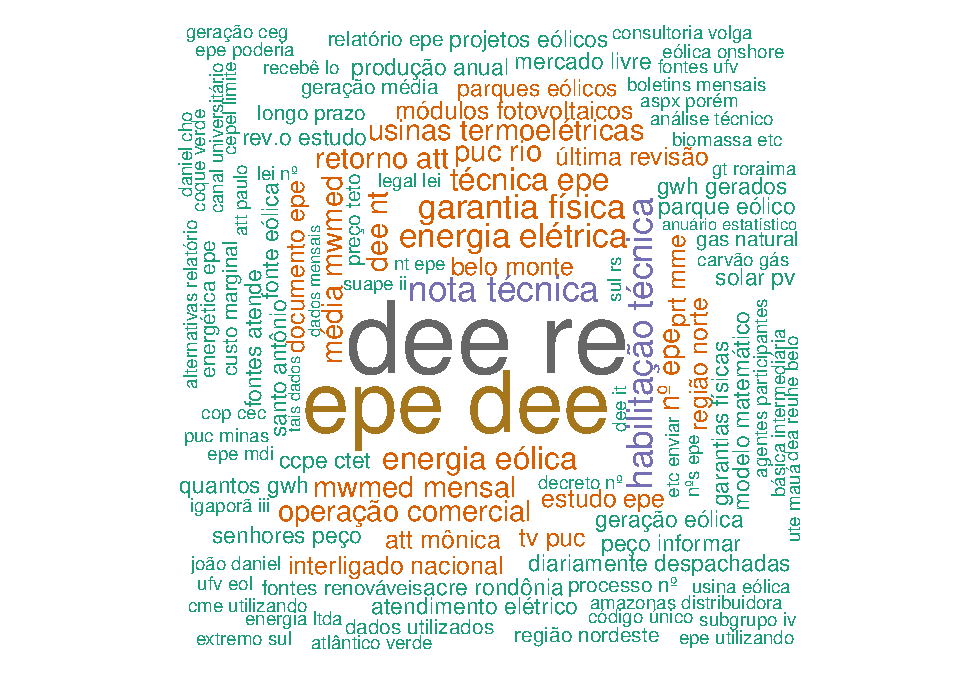
\includegraphics{markdown_v21_files/figure-latex/wordcloud_bigram_DIR01_semstopwords-1.pdf}

\begin{Shaded}
\begin{Highlighting}[]
\NormalTok{## DGC}
\CommentTok{#jpeg("XX_wordclou_tfidf_dir02_DGC.jpeg")}
\NormalTok{nuvem2.}\DecValTok{2}\NormalTok{ =}\StringTok{ }
\NormalTok{plot_diretorias_tf_dif_bigram2 }\OperatorTok
\StringTok{  }\KeywordTok{filter}\NormalTok{(DIRETORIA }\OperatorTok{==}\StringTok{ "DGC"}\NormalTok{) }\OperatorTok
\StringTok{  }\KeywordTok{select}\NormalTok{(}\OperatorTok{-}\NormalTok{DIRETORIA, }\DataTypeTok{word =}\NormalTok{ BIGRAM,}\DataTypeTok{freq =}\NormalTok{ tf_idf) }\OperatorTok
\StringTok{  }\CommentTok{#top_n(150, freq) %>%}
\StringTok{  }\KeywordTok{as.data.frame}\NormalTok{() }

\KeywordTok{set.seed}\NormalTok{(}\DecValTok{95654}\NormalTok{)}
\KeywordTok{wordcloud}\NormalTok{(}\DataTypeTok{words =}\NormalTok{ nuvem2.}\DecValTok{2}\OperatorTok{$}\NormalTok{word, }\DataTypeTok{freq =}\NormalTok{ nuvem2.}\DecValTok{2}\OperatorTok{$}\NormalTok{freq,}
          \DataTypeTok{max.words=}\DecValTok{250}\NormalTok{, }\DataTypeTok{random.order=}\OtherTok{FALSE}\NormalTok{, }\DataTypeTok{rot.per=}\FloatTok{0.35}\NormalTok{, }
          \DataTypeTok{colors=}\KeywordTok{brewer.pal}\NormalTok{(}\DecValTok{10}\NormalTok{, }\StringTok{"Dark2"}\NormalTok{))}
\end{Highlighting}
\end{Shaded}


\includegraphics{markdown_v21_files/figure-latex/wordcloud_bigram_DIR02_semstopwords-1.pdf}

\begin{Shaded}
\begin{Highlighting}[]
\NormalTok{## DEA}
\CommentTok{#jpeg("XX_wordclou_tfidf_dir03_DEA.jpeg")}
\NormalTok{nuvem3.}\DecValTok{2}\NormalTok{ =}\StringTok{ }
\NormalTok{plot_diretorias_tf_dif_bigram2 }\OperatorTok
\StringTok{  }\KeywordTok{filter}\NormalTok{(DIRETORIA }\OperatorTok{==}\StringTok{ "DEA"}\NormalTok{) }\OperatorTok
\StringTok{  }\KeywordTok{select}\NormalTok{(}\OperatorTok{-}\NormalTok{DIRETORIA, }\DataTypeTok{word =}\NormalTok{ BIGRAM,}\DataTypeTok{freq =}\NormalTok{ tf_idf) }\OperatorTok
\StringTok{  }\CommentTok{#top_n(150, freq) %>%}
\StringTok{  }\KeywordTok{as.data.frame}\NormalTok{() }

\KeywordTok{set.seed}\NormalTok{(}\DecValTok{543453}\NormalTok{)}
\KeywordTok{wordcloud}\NormalTok{(}\DataTypeTok{words =}\NormalTok{ nuvem3.}\DecValTok{2}\OperatorTok{$}\NormalTok{word, }\DataTypeTok{freq =}\NormalTok{ nuvem3.}\DecValTok{2}\OperatorTok{$}\NormalTok{freq,}
          \DataTypeTok{max.words=}\DecValTok{250}\NormalTok{, }\DataTypeTok{random.order=}\OtherTok{FALSE}\NormalTok{, }\DataTypeTok{rot.per=}\FloatTok{0.35}\NormalTok{, }
          \DataTypeTok{colors=}\KeywordTok{brewer.pal}\NormalTok{(}\DecValTok{10}\NormalTok{, }\StringTok{"Dark2"}\NormalTok{))}
\end{Highlighting}
\end{Shaded}

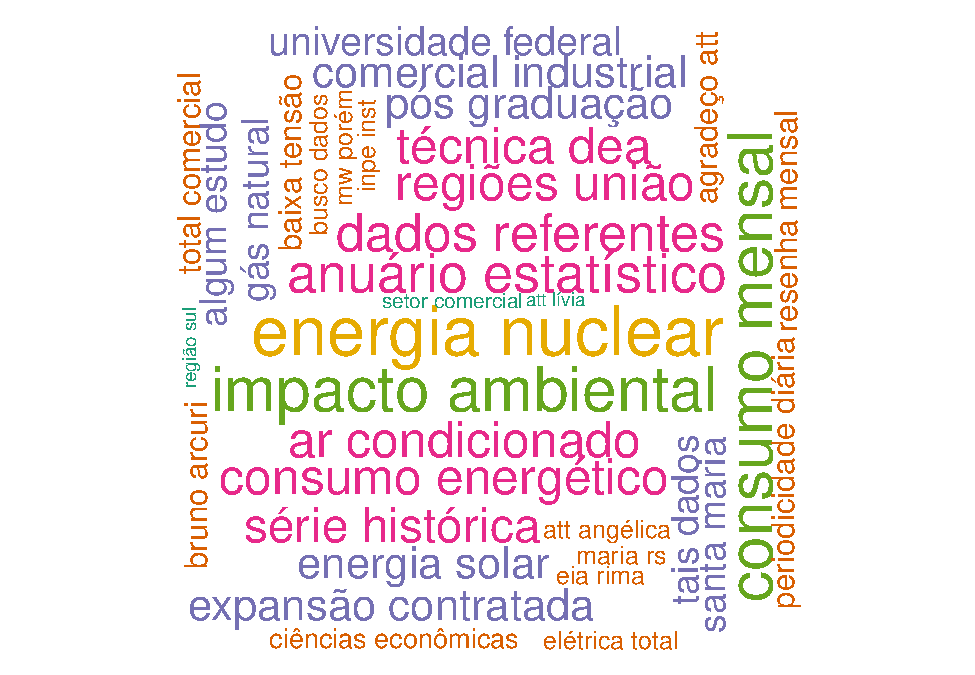
\includegraphics{markdown_v21_files/figure-latex/wordcloud_bigram_DIR03_semstopwords-1.pdf}

\begin{Shaded}
\begin{Highlighting}[]
\NormalTok{## DPG}
\CommentTok{#jpeg("XX_wordclou_tfidf_dir04_DPG.jpeg")}
\NormalTok{nuvem4.}\DecValTok{2}\NormalTok{ =}\StringTok{ }
\NormalTok{plot_diretorias_tf_dif_bigram2 }\OperatorTok
\StringTok{  }\KeywordTok{filter}\NormalTok{(DIRETORIA }\OperatorTok{==}\StringTok{ "DPG"}\NormalTok{) }\OperatorTok
\StringTok{  }\KeywordTok{select}\NormalTok{(}\OperatorTok{-}\NormalTok{DIRETORIA, }\DataTypeTok{word =}\NormalTok{ BIGRAM,}\DataTypeTok{freq =}\NormalTok{ tf_idf) }\OperatorTok
\StringTok{  }\CommentTok{#top_n(150, freq) %>%}
\StringTok{  }\KeywordTok{as.data.frame}\NormalTok{() }

\KeywordTok{set.seed}\NormalTok{(}\DecValTok{75437}\NormalTok{)}
\KeywordTok{wordcloud}\NormalTok{(}\DataTypeTok{words =}\NormalTok{ nuvem4.}\DecValTok{2}\OperatorTok{$}\NormalTok{word, }\DataTypeTok{freq =}\NormalTok{ nuvem4.}\DecValTok{2}\OperatorTok{$}\NormalTok{freq, }\DataTypeTok{min.freq =} \FloatTok{0.1}\NormalTok{,}
          \DataTypeTok{max.words=}\DecValTok{250}\NormalTok{, }\DataTypeTok{random.order=}\OtherTok{FALSE}\NormalTok{, }\DataTypeTok{rot.per=}\FloatTok{0.35}\NormalTok{, }
          \DataTypeTok{colors=}\KeywordTok{brewer.pal}\NormalTok{(}\DecValTok{10}\NormalTok{, }\StringTok{"Dark2"}\NormalTok{))}
\end{Highlighting}
\end{Shaded}

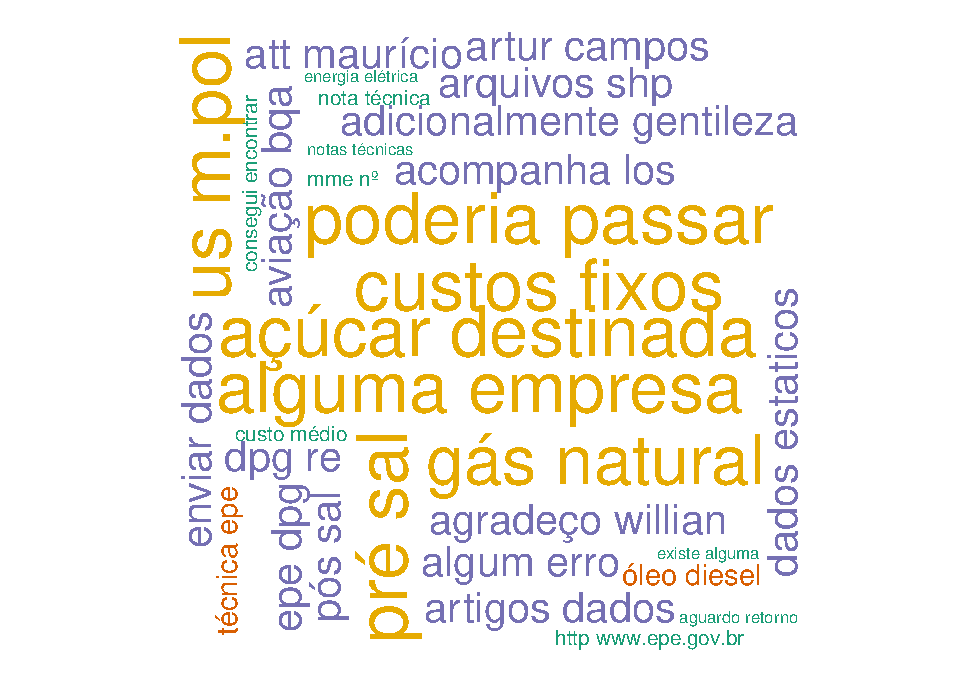
\includegraphics{markdown_v21_files/figure-latex/wordcloud_bigram_DIR04_semstopwords-1.pdf}

\begin{Shaded}
\begin{Highlighting}[]
\NormalTok{## OUTROS}
\CommentTok{#jpeg("XX_wordclou_tfidf_dir05_OUTROS.jpeg")}
\NormalTok{nuvem5.}\DecValTok{2}\NormalTok{ =}\StringTok{ }
\NormalTok{plot_diretorias_tf_dif_bigram2 }\OperatorTok
\StringTok{  }\KeywordTok{filter}\NormalTok{(DIRETORIA }\OperatorTok{==}\StringTok{ "OUTROS"}\NormalTok{) }\OperatorTok
\StringTok{  }\KeywordTok{select}\NormalTok{(}\OperatorTok{-}\NormalTok{DIRETORIA, }\DataTypeTok{word =}\NormalTok{ BIGRAM,}\DataTypeTok{freq =}\NormalTok{ tf_idf) }\OperatorTok
\StringTok{  }\CommentTok{#top_n(150, freq) %>%}
\StringTok{  }\KeywordTok{as.data.frame}\NormalTok{() }

\KeywordTok{set.seed}\NormalTok{(}\DecValTok{75437}\NormalTok{)}
\KeywordTok{wordcloud}\NormalTok{(}\DataTypeTok{words =}\NormalTok{ nuvem5.}\DecValTok{2}\OperatorTok{$}\NormalTok{word, }\DataTypeTok{freq =}\NormalTok{ nuvem5.}\DecValTok{2}\OperatorTok{$}\NormalTok{freq, }\DataTypeTok{min.freq =} \FloatTok{0.1}\NormalTok{,}
          \DataTypeTok{max.words=}\DecValTok{250}\NormalTok{, }\DataTypeTok{random.order=}\OtherTok{FALSE}\NormalTok{, }\DataTypeTok{rot.per=}\FloatTok{0.35}\NormalTok{, }
          \DataTypeTok{colors=}\KeywordTok{brewer.pal}\NormalTok{(}\DecValTok{10}\NormalTok{, }\StringTok{"Dark2"}\NormalTok{))}
\end{Highlighting}
\end{Shaded}

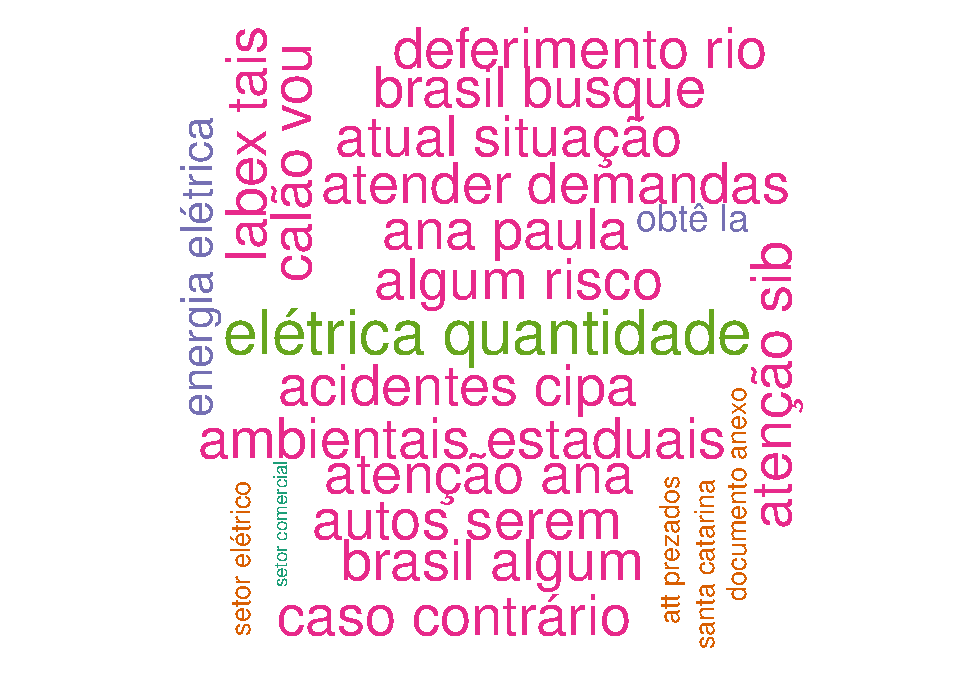
\includegraphics{markdown_v21_files/figure-latex/wordcloud_bigram_DIR05_semstopwords-1.pdf}

\begin{Shaded}
\begin{Highlighting}[]
\CommentTok{#View(head(plot_diretoria_palavras))}
\NormalTok{library(wordcloud2)}

\NormalTok{plot_diretorias_tf_dif_bigram2 = bigrams2 %>%}
\NormalTok{  select(BIGRAM,n,DIRETORIA) %>%}
\NormalTok{  bind_tf_idf(BIGRAM, DIRETORIA, n) %>%}
\NormalTok{  arrange(desc(tf_idf)) %>%}
\NormalTok{  mutate(BIGRAM = factor(BIGRAM, levels = rev(unique(BIGRAM)))) %>%}
\NormalTok{  mutate(DIRETORIA = factor(DIRETORIA,levels=c(}\StringTok{"DEA"}\NormalTok{,}\StringTok{"DEE"}\NormalTok{,}\StringTok{"DGC"}\NormalTok{,}\StringTok{"DPG"}\NormalTok{,}\StringTok{"OUTROS"}\NormalTok{))) %>%}
\NormalTok{  select(BIGRAM, tf_idf, DIRETORIA)}
  

\CommentTok{## DEE}
\CommentTok{#jpeg("XX_wordclou_tfidf_dir01_DEE.jpeg")}
\NormalTok{set.seed(233115)}
\NormalTok{plot_diretorias_tf_dif_bigram2 %>%}
\NormalTok{  filter(DIRETORIA == }\StringTok{"DEE"}\NormalTok{) %>%}
\NormalTok{  top_n(150, tf_idf) %>%}
\NormalTok{  wordcloud2(shuffle = TRUE, }
\NormalTok{             color = }\StringTok{"random-dark"}\NormalTok{,}
\NormalTok{             shape = }\StringTok{"circle"}\NormalTok{)}

\CommentTok{## DGC}
\CommentTok{#jpeg("XX_wordclou_tfidf_dir02_DGC.jpeg")}
\NormalTok{set.seed(233115)}
\NormalTok{plot_diretorias_tf_dif_bigram2 %>%}
\NormalTok{  filter(DIRETORIA == }\StringTok{"DGC"}\NormalTok{) %>%}
\NormalTok{  top_n(150, tf_idf) %>%}
\NormalTok{  wordcloud2()}

\CommentTok{## DEA}
\CommentTok{#jpeg("XX_wordclou_tfidf_dir03_DEA.jpeg")}
\NormalTok{set.seed(233115)}
\NormalTok{plot_diretorias_tf_dif_bigram2 %>%}
\NormalTok{  filter(DIRETORIA == }\StringTok{"DEA"}\NormalTok{) %>%}
\NormalTok{  top_n(150, tf_idf) %>%}
\NormalTok{  wordcloud2()}

\CommentTok{## DPG}
\CommentTok{#jpeg("XX_wordclou_tfidf_dir04_DPG.jpeg")}
\NormalTok{set.seed(233115)}
\NormalTok{plot_diretorias_tf_dif_bigram2 %>%}
\NormalTok{  filter(DIRETORIA == }\StringTok{"DPG"}\NormalTok{) %>%}
\NormalTok{  top_n(150, tf_idf) %>%}
\NormalTok{  wordcloud2()}

\CommentTok{## OUTROS}
\CommentTok{#jpeg("XX_wordclou_tfidf_dir05_OUTROS.jpeg")}
\NormalTok{set.seed(233115)}
\NormalTok{plot_diretorias_tf_dif_bigram2 %>%}
\NormalTok{  filter(DIRETORIA == }\StringTok{"OUTROS"}\NormalTok{) %>%}
\NormalTok{  top_n(150, tf_idf) %>%}
\NormalTok{  wordcloud2()}
\end{Highlighting}
\end{Shaded}

\paragraph{Gráfico da estatística tf\_idf c/ remoção de
stopwords}\label{grafico-da-estatistica-tf_idf-c-remocao-de-stopwords}

\begin{Shaded}
\begin{Highlighting}[]
\NormalTok{plot_diretorias_tf_dif_bigram2 }\OperatorTok
\KeywordTok{group_by}\NormalTok{(DIRETORIA) }\OperatorTok
\KeywordTok{top_n}\NormalTok{(}\DecValTok{10}\NormalTok{, tf_idf) }\OperatorTok
\KeywordTok{ungroup}\NormalTok{() }\OperatorTok
\KeywordTok{mutate}\NormalTok{(}\DataTypeTok{BIGRAM =} \KeywordTok{reorder}\NormalTok{(BIGRAM, tf_idf)) }\OperatorTok
\KeywordTok{ggplot}\NormalTok{(}\KeywordTok{aes}\NormalTok{(BIGRAM, tf_idf, }\DataTypeTok{fill =}\NormalTok{ DIRETORIA)) }\OperatorTok{+}
\KeywordTok{geom_col}\NormalTok{(}\DataTypeTok{show.legend =} \OtherTok{FALSE}\NormalTok{) }\OperatorTok{+}
\KeywordTok{labs}\NormalTok{(}\DataTypeTok{x =} \OtherTok{NULL}\NormalTok{, }\DataTypeTok{y =} \StringTok{"tf-idf"}\NormalTok{) }\OperatorTok{+}
\KeywordTok{facet_wrap}\NormalTok{(}\OperatorTok{~}\NormalTok{DIRETORIA, }\DataTypeTok{ncol =} \DecValTok{2}\NormalTok{, }\DataTypeTok{scales =} \StringTok{"free"}\NormalTok{) }\OperatorTok{+}
\KeywordTok{coord_flip}\NormalTok{() }\OperatorTok{+}\StringTok{ }
\KeywordTok{scale_y_continuous}\NormalTok{(}\DataTypeTok{labels=}\NormalTok{gcomma)}
\end{Highlighting}
\end{Shaded}

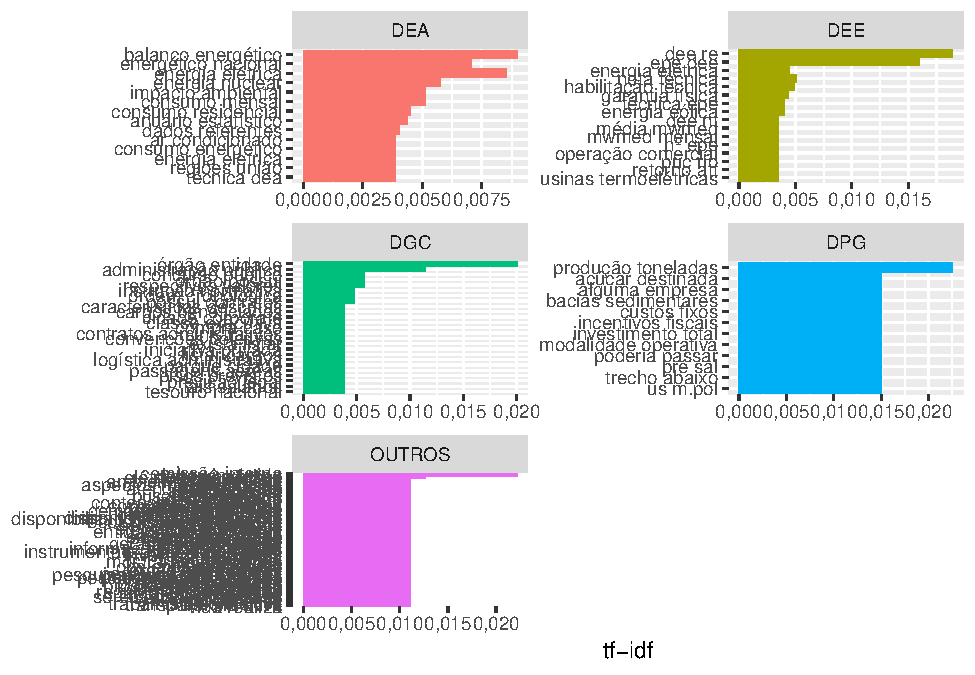
\includegraphics{markdown_v21_files/figure-latex/unnamed-chunk-43-1.pdf}

\paragraph{Nuvem de palavras por diretoria - s/ steeming e/ou stopwords
-
trigram}\label{nuvem-de-palavras-por-diretoria---s-steeming-eou-stopwords---trigram}

\begin{Shaded}
\begin{Highlighting}[]
\CommentTok{#View(head(plot_diretoria_palavras))}
\KeywordTok{library}\NormalTok{(wordcloud)}
\NormalTok{plot_diretorias_tf_dif_trigram =}\StringTok{ }\NormalTok{DB }\OperatorTok
\StringTok{  }\KeywordTok{select}\NormalTok{(DESCRI_PEDIDO,DIRETORIA) }\OperatorTok
\StringTok{  }\KeywordTok{unnest_tokens}\NormalTok{(TRIGRAM, DESCRI_PEDIDO, }\DataTypeTok{token =} \StringTok{"ngrams"}\NormalTok{, }\DataTypeTok{n =} \DecValTok{3}\NormalTok{) }\OperatorTok
\StringTok{  }\KeywordTok{count}\NormalTok{(DIRETORIA, TRIGRAM, }\DataTypeTok{sort =} \OtherTok{TRUE}\NormalTok{) }\OperatorTok
\StringTok{  }\KeywordTok{bind_tf_idf}\NormalTok{(TRIGRAM, DIRETORIA, n) }\OperatorTok
\StringTok{  }\KeywordTok{arrange}\NormalTok{(}\KeywordTok{desc}\NormalTok{(tf_idf)) }\OperatorTok
\StringTok{  }\KeywordTok{mutate}\NormalTok{(}\DataTypeTok{TRIGRAM =} \KeywordTok{factor}\NormalTok{(TRIGRAM, }\DataTypeTok{levels =} \KeywordTok{rev}\NormalTok{(}\KeywordTok{unique}\NormalTok{(TRIGRAM)))) }\OperatorTok
\StringTok{  }\KeywordTok{mutate}\NormalTok{(}\DataTypeTok{DIRETORIA =} \KeywordTok{factor}\NormalTok{(DIRETORIA,}\DataTypeTok{levels=}\KeywordTok{c}\NormalTok{(}\StringTok{"DEA"}\NormalTok{,}\StringTok{"DEE"}\NormalTok{,}\StringTok{"DGC"}\NormalTok{,}\StringTok{"DPG"}\NormalTok{,}\StringTok{"OUTROS"}\NormalTok{))) }\OperatorTok
\StringTok{  }\KeywordTok{select}\NormalTok{(TRIGRAM, tf_idf, DIRETORIA)}
\end{Highlighting}
\end{Shaded}

\begin{Shaded}
\begin{Highlighting}[]
\NormalTok{## DEE}
\CommentTok{#jpeg("wordcloud_tfidf_dir01_DEE_trigram_comstop_semstemming.jpeg")}
\NormalTok{nuvem1.}\DecValTok{3}\NormalTok{ =}\StringTok{ }
\NormalTok{plot_diretorias_tf_dif_trigram }\OperatorTok
\StringTok{  }\KeywordTok{filter}\NormalTok{(DIRETORIA }\OperatorTok{==}\StringTok{ "DEE"}\NormalTok{) }\OperatorTok
\StringTok{  }\KeywordTok{select}\NormalTok{(}\OperatorTok{-}\NormalTok{DIRETORIA, }\DataTypeTok{word =}\NormalTok{ TRIGRAM,}\DataTypeTok{freq =}\NormalTok{ tf_idf) }\OperatorTok
\StringTok{  }\CommentTok{#top_n(150, freq) %>%}
\StringTok{  }\KeywordTok{as.data.frame}\NormalTok{() }

\KeywordTok{set.seed}\NormalTok{(}\DecValTok{8835}\NormalTok{)}
\KeywordTok{wordcloud}\NormalTok{(}\DataTypeTok{words =}\NormalTok{ nuvem1.}\DecValTok{3}\OperatorTok{$}\NormalTok{word, }\DataTypeTok{freq =}\NormalTok{ nuvem1.}\DecValTok{3}\OperatorTok{$}\NormalTok{freq, }\DataTypeTok{min.freq =} \FloatTok{0.2}\NormalTok{,}
          \DataTypeTok{max.words=}\DecValTok{250}\NormalTok{, }\DataTypeTok{random.order=}\OtherTok{FALSE}\NormalTok{, }\DataTypeTok{rot.per=}\FloatTok{0.35}\NormalTok{, }
          \DataTypeTok{colors=}\KeywordTok{brewer.pal}\NormalTok{(}\DecValTok{10}\NormalTok{, }\StringTok{"Dark2"}\NormalTok{))}
\end{Highlighting}
\end{Shaded}

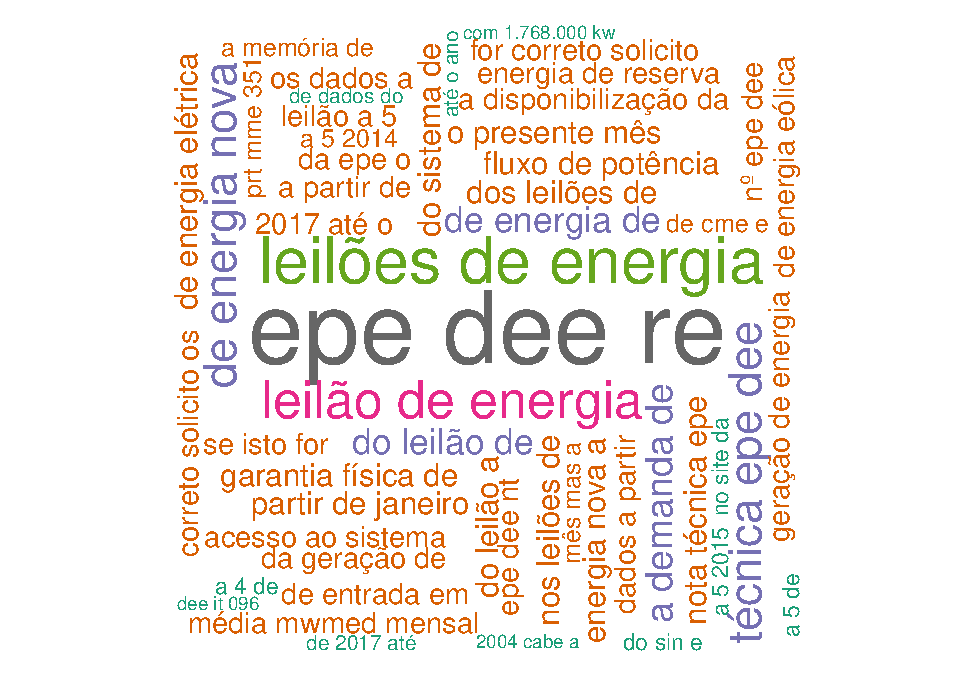
\includegraphics{markdown_v21_files/figure-latex/wordcloud_trigram_DIR01_comstopwords-1.pdf}

\begin{Shaded}
\begin{Highlighting}[]
\CommentTok{#dev.off()}
\end{Highlighting}
\end{Shaded}

\begin{Shaded}
\begin{Highlighting}[]
\NormalTok{## DGC}
\CommentTok{#jpeg("wordcloud_tfidf_dir02_DGC_trigram_comstop_semstemming.jpeg")}
\NormalTok{nuvem2.}\DecValTok{3}\NormalTok{ =}\StringTok{ }
\NormalTok{plot_diretorias_tf_dif_trigram }\OperatorTok
\StringTok{  }\KeywordTok{filter}\NormalTok{(DIRETORIA }\OperatorTok{==}\StringTok{ "DGC"}\NormalTok{) }\OperatorTok
\StringTok{  }\KeywordTok{select}\NormalTok{(}\OperatorTok{-}\NormalTok{DIRETORIA, }\DataTypeTok{word =}\NormalTok{ TRIGRAM,}\DataTypeTok{freq =}\NormalTok{ tf_idf) }\OperatorTok
\StringTok{  }\CommentTok{#top_n(150, freq) %>%}
\StringTok{  }\KeywordTok{as.data.frame}\NormalTok{() }

\KeywordTok{set.seed}\NormalTok{(}\DecValTok{1273}\NormalTok{)}
\KeywordTok{wordcloud}\NormalTok{(}\DataTypeTok{words =}\NormalTok{ nuvem2.}\DecValTok{3}\OperatorTok{$}\NormalTok{word, }\DataTypeTok{freq =}\NormalTok{ nuvem2.}\DecValTok{3}\OperatorTok{$}\NormalTok{freq, }\DataTypeTok{min.freq =} \FloatTok{0.2}\NormalTok{,}
          \DataTypeTok{max.words=}\DecValTok{250}\NormalTok{, }\DataTypeTok{random.order=}\OtherTok{FALSE}\NormalTok{, }\DataTypeTok{rot.per=}\FloatTok{0.35}\NormalTok{, }
          \DataTypeTok{colors=}\KeywordTok{brewer.pal}\NormalTok{(}\DecValTok{10}\NormalTok{, }\StringTok{"Dark2"}\NormalTok{))}
\end{Highlighting}
\end{Shaded}

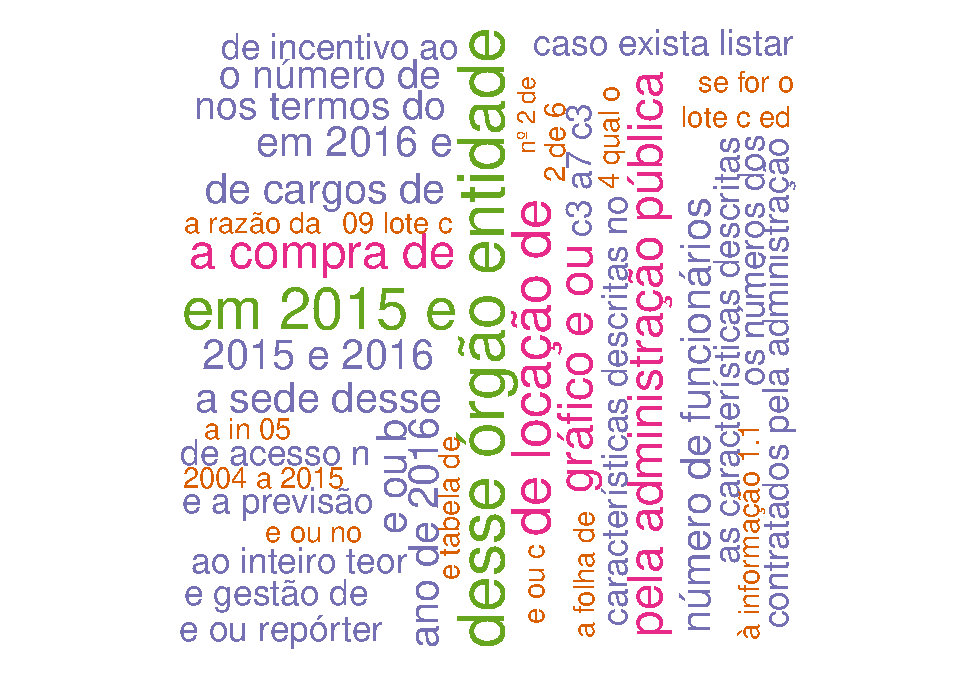
\includegraphics{markdown_v21_files/figure-latex/wordcloud_trigram_DIR02_comstopwords-1.pdf}

\begin{Shaded}
\begin{Highlighting}[]
\NormalTok{## DEA}
\CommentTok{#jpeg("XX_wordclou_tfidf_dir03_DEA_trigram_comstop_semstemming.jpeg")}
\NormalTok{nuvem3.}\DecValTok{3}\NormalTok{ =}\StringTok{ }
\NormalTok{plot_diretorias_tf_dif_trigram }\OperatorTok
\StringTok{  }\KeywordTok{filter}\NormalTok{(DIRETORIA }\OperatorTok{==}\StringTok{ "DEA"}\NormalTok{) }\OperatorTok
\StringTok{  }\KeywordTok{select}\NormalTok{(}\OperatorTok{-}\NormalTok{DIRETORIA, }\DataTypeTok{word =}\NormalTok{ TRIGRAM,}\DataTypeTok{freq =}\NormalTok{ tf_idf) }\OperatorTok
\StringTok{  }\CommentTok{#top_n(150, freq) %>%}
\StringTok{  }\KeywordTok{as.data.frame}\NormalTok{() }

\KeywordTok{set.seed}\NormalTok{(}\DecValTok{543453}\NormalTok{)}
\KeywordTok{wordcloud}\NormalTok{(}\DataTypeTok{words =}\NormalTok{ nuvem3.}\DecValTok{3}\OperatorTok{$}\NormalTok{word, }\DataTypeTok{freq =}\NormalTok{ nuvem3.}\DecValTok{3}\OperatorTok{$}\NormalTok{freq,}
          \DataTypeTok{max.words=}\DecValTok{250}\NormalTok{, }\DataTypeTok{random.order=}\OtherTok{FALSE}\NormalTok{, }\DataTypeTok{rot.per=}\FloatTok{0.35}\NormalTok{, }
          \DataTypeTok{colors=}\KeywordTok{brewer.pal}\NormalTok{(}\DecValTok{10}\NormalTok{, }\StringTok{"Dark2"}\NormalTok{))}
\end{Highlighting}
\end{Shaded}

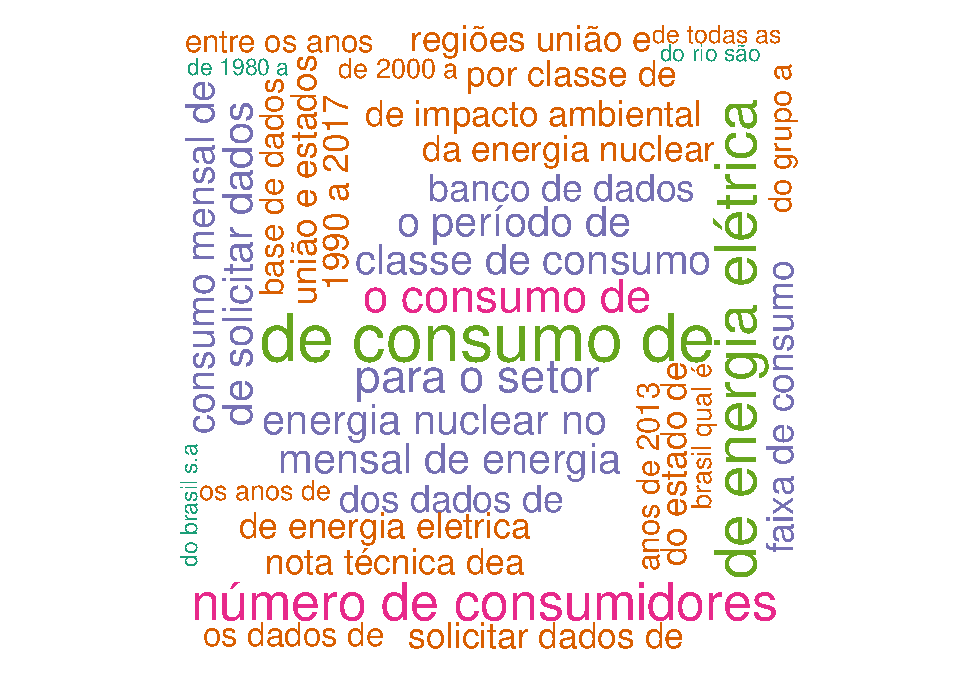
\includegraphics{markdown_v21_files/figure-latex/wordcloud_trigram_DIR03_comstopwords-1.pdf}

\begin{Shaded}
\begin{Highlighting}[]
\NormalTok{## DPG}
\CommentTok{#jpeg("XX_wordclou_tfidf_dir04_DPG_trigram_comstop_semstemming.jpeg")}
\NormalTok{nuvem4.}\DecValTok{3}\NormalTok{ =}\StringTok{ }
\NormalTok{plot_diretorias_tf_dif_trigram }\OperatorTok
\StringTok{  }\KeywordTok{filter}\NormalTok{(DIRETORIA }\OperatorTok{==}\StringTok{ "DPG"}\NormalTok{) }\OperatorTok
\StringTok{  }\KeywordTok{select}\NormalTok{(}\OperatorTok{-}\NormalTok{DIRETORIA, }\DataTypeTok{word =}\NormalTok{ TRIGRAM,}\DataTypeTok{freq =}\NormalTok{ tf_idf) }\OperatorTok
\StringTok{  }\CommentTok{#top_n(150, freq) %>%}
\StringTok{  }\KeywordTok{as.data.frame}\NormalTok{() }

\KeywordTok{set.seed}\NormalTok{(}\DecValTok{75437}\NormalTok{)}
\KeywordTok{wordcloud}\NormalTok{(}\DataTypeTok{words =}\NormalTok{ nuvem4.}\DecValTok{3}\OperatorTok{$}\NormalTok{word, }\DataTypeTok{freq =}\NormalTok{ nuvem4.}\DecValTok{3}\OperatorTok{$}\NormalTok{freq, }\DataTypeTok{min.freq =} \FloatTok{0.1}\NormalTok{,}
          \DataTypeTok{max.words=}\DecValTok{250}\NormalTok{, }\DataTypeTok{random.order=}\OtherTok{FALSE}\NormalTok{, }\DataTypeTok{rot.per=}\FloatTok{0.35}\NormalTok{, }
          \DataTypeTok{colors=}\KeywordTok{brewer.pal}\NormalTok{(}\DecValTok{10}\NormalTok{, }\StringTok{"Dark2"}\NormalTok{))}
\end{Highlighting}
\end{Shaded}

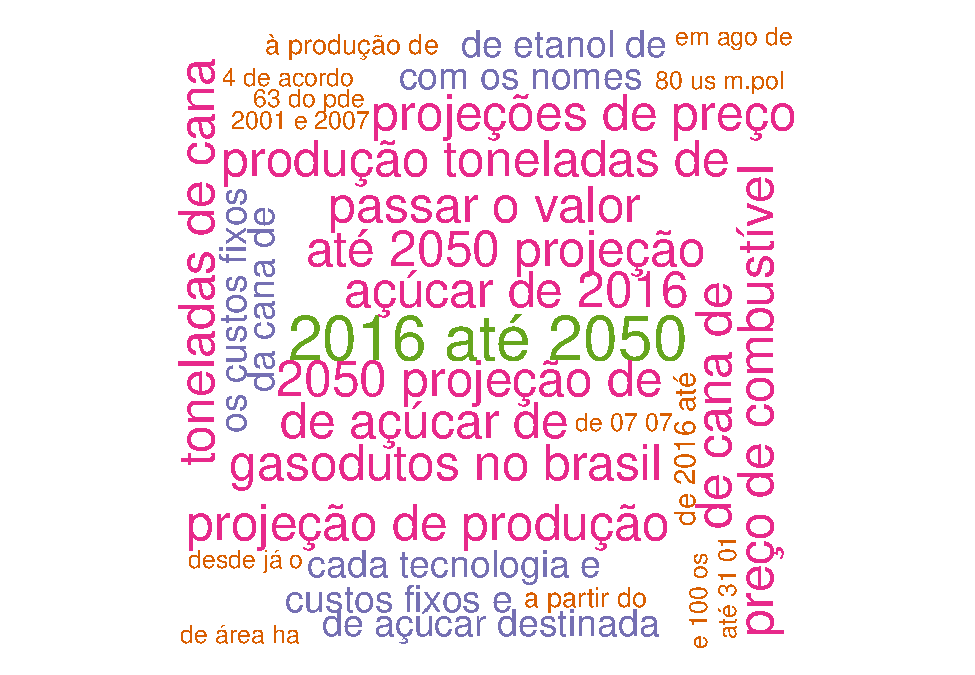
\includegraphics{markdown_v21_files/figure-latex/wordcloud_trigram_DIR04_comstopwords-1.pdf}

\begin{Shaded}
\begin{Highlighting}[]
\NormalTok{## OUTROS}
\CommentTok{#jpeg("XX_wordclou_tfidf_dir05_OUTROS_trigram_comstop_semstemming.jpeg")}
\NormalTok{nuvem5.}\DecValTok{3}\NormalTok{ =}\StringTok{ }
\NormalTok{plot_diretorias_tf_dif_trigram }\OperatorTok
\StringTok{  }\KeywordTok{filter}\NormalTok{(DIRETORIA }\OperatorTok{==}\StringTok{ "OUTROS"}\NormalTok{) }\OperatorTok
\StringTok{  }\KeywordTok{select}\NormalTok{(}\OperatorTok{-}\NormalTok{DIRETORIA, }\DataTypeTok{word =}\NormalTok{ TRIGRAM,}\DataTypeTok{freq =}\NormalTok{ tf_idf) }\OperatorTok
\StringTok{  }\CommentTok{#top_n(150, freq) %>%}
\StringTok{  }\KeywordTok{as.data.frame}\NormalTok{() }

\KeywordTok{set.seed}\NormalTok{(}\DecValTok{1235}\NormalTok{)}
\KeywordTok{wordcloud}\NormalTok{(}\DataTypeTok{words =}\NormalTok{ nuvem5.}\DecValTok{3}\OperatorTok{$}\NormalTok{word, }\DataTypeTok{freq =}\NormalTok{ nuvem5.}\DecValTok{3}\OperatorTok{$}\NormalTok{freq,}
          \DataTypeTok{max.words=}\DecValTok{100}\NormalTok{, }\DataTypeTok{random.order=}\OtherTok{FALSE}\NormalTok{, }\DataTypeTok{rot.per=}\FloatTok{0.35}\NormalTok{, }
          \DataTypeTok{colors=}\KeywordTok{brewer.pal}\NormalTok{(}\DecValTok{10}\NormalTok{, }\StringTok{"Dark2"}\NormalTok{))}
\end{Highlighting}
\end{Shaded}

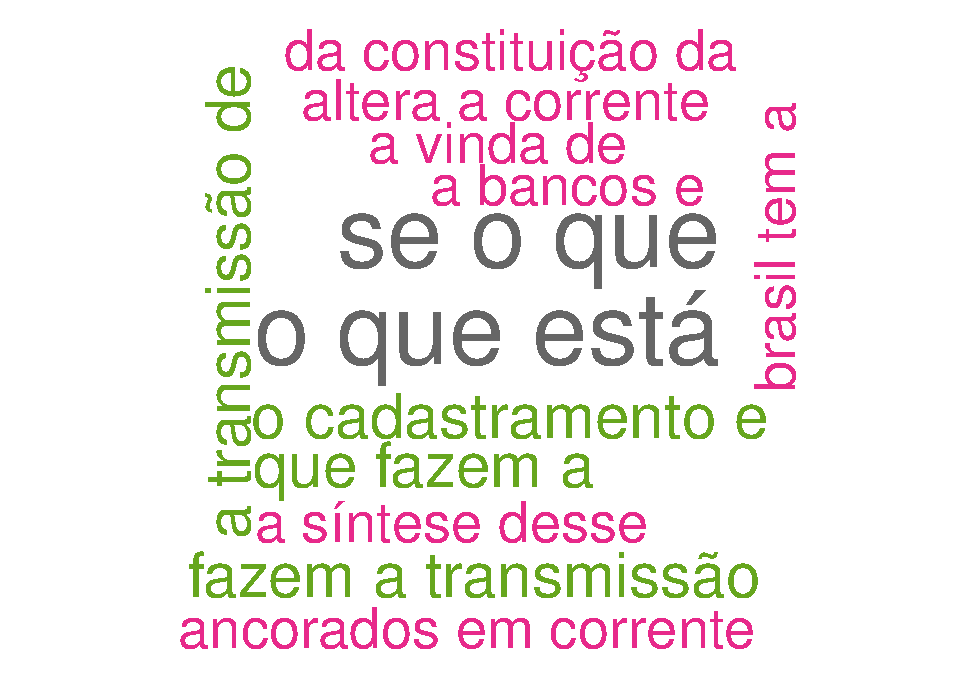
\includegraphics{markdown_v21_files/figure-latex/wordcloud_trigram_DIR05_comstopwords-1.pdf}

\begin{Shaded}
\begin{Highlighting}[]
\CommentTok{#View(head(plot_diretoria_palavras))}
\NormalTok{library(wordcloud2)}

\NormalTok{plot_diretorias_tf_dif_trigram = DB %>%}
\NormalTok{  select(DESCRI_PEDIDO,DIRETORIA) %>%}
\NormalTok{  unnest_tokens(TRIGRAM, DESCRI_PEDIDO, token = }\StringTok{"ngrams"}\NormalTok{, n = 3) %>%}
\NormalTok{  count(DIRETORIA, TRIGRAM, sort = TRUE) %>%}
\NormalTok{  bind_tf_idf(TRIGRAM, DIRETORIA, n) %>%}
\NormalTok{  arrange(desc(tf_idf)) %>%}
\NormalTok{  mutate(TRIGRAM = factor(TRIGRAM, levels = rev(unique(TRIGRAM)))) %>%}
\NormalTok{  mutate(DIRETORIA = factor(DIRETORIA,levels=c(}\StringTok{"DEA"}\NormalTok{,}\StringTok{"DEE"}\NormalTok{,}\StringTok{"DGC"}\NormalTok{,}\StringTok{"DPG"}\NormalTok{,}\StringTok{"OUTROS"}\NormalTok{))) %>%}
\NormalTok{  select(TRIGRAM, tf_idf, DIRETORIA)}
  

\CommentTok{## DEE}
\CommentTok{#jpeg("XX_wordclou_tfidf_dir01_DEE.jpeg")}
\NormalTok{set.seed(233115)}
\NormalTok{plot_diretorias_tf_dif_trigram %>%}
\NormalTok{  filter(DIRETORIA == }\StringTok{"DEE"}\NormalTok{) %>%}
\NormalTok{  top_n(150, tf_idf) %>%}
\NormalTok{  wordcloud2(shuffle = TRUE, }
\NormalTok{             color = }\StringTok{"random-dark"}\NormalTok{,}
\NormalTok{             shape = }\StringTok{"circle"}\NormalTok{)}

\CommentTok{## DGC}
\CommentTok{#jpeg("XX_wordclou_tfidf_dir02_DGC.jpeg")}
\NormalTok{set.seed(233115)}
\NormalTok{plot_diretorias_tf_dif_trigram %>%}
\NormalTok{  filter(DIRETORIA == }\StringTok{"DGC"}\NormalTok{) %>%}
\NormalTok{  top_n(150, tf_idf) %>%}
\NormalTok{  wordcloud2()}

\CommentTok{## DEA}
\CommentTok{#jpeg("XX_wordclou_tfidf_dir03_DEA.jpeg")}
\NormalTok{set.seed(233115)}
\NormalTok{plot_diretorias_tf_dif_trigram %>%}
\NormalTok{  filter(DIRETORIA == }\StringTok{"DEA"}\NormalTok{) %>%}
\NormalTok{  top_n(150, tf_idf) %>%}
\NormalTok{  wordcloud2()}

\CommentTok{## DPG}
\CommentTok{#jpeg("XX_wordclou_tfidf_dir04_DPG.jpeg")}
\NormalTok{set.seed(233115)}
\NormalTok{plot_diretorias_tf_dif_trigram %>%}
\NormalTok{  filter(DIRETORIA == }\StringTok{"DPG"}\NormalTok{) %>%}
\NormalTok{  top_n(150, tf_idf) %>%}
\NormalTok{  wordcloud2()}
  
\CommentTok{## OUTROS}
\CommentTok{#jpeg("XX_wordclou_tfidf_dir05_OUTROS.jpeg")}
\NormalTok{set.seed(233115)}
\NormalTok{plot_diretorias_tf_dif_trigram %>%}
\NormalTok{  filter(DIRETORIA == }\StringTok{"OUTROS"}\NormalTok{) %>%}
\NormalTok{  top_n(150, tf_idf) %>%}
\NormalTok{  wordcloud2()  }
\end{Highlighting}
\end{Shaded}

\subsection{ANEXOS}\label{anexos}

\begin{itemize}
\tightlist
\item
  Anexo 01: Tabela - Exemplo amostral da tabela unificada
\end{itemize}

\begin{Shaded}
\begin{Highlighting}[]
\NormalTok{DB[}\KeywordTok{c}\NormalTok{(}\DecValTok{32}\NormalTok{,}\DecValTok{50}\NormalTok{,}\DecValTok{66}\NormalTok{),}\KeywordTok{c}\NormalTok{(}\OperatorTok{-}\DecValTok{1}\NormalTok{,}\OperatorTok{-}\DecValTok{3}\NormalTok{,}\OperatorTok{-}\DecValTok{5}\NormalTok{,}\OperatorTok{-}\DecValTok{6}\NormalTok{,}\OperatorTok{-}\DecValTok{9}\NormalTok{)] }\OperatorTok
\StringTok{  }\KeywordTok{select}\NormalTok{(DATA_PEDIDO, DATA_RESPOSTA, DIRETORIA, DESCRI_PEDIDO) }\OperatorTok
\KeywordTok{kable}\NormalTok{(}\StringTok{"latex"}\NormalTok{, }\DataTypeTok{caption =} \StringTok{"Amostra dos dados a serem pré-processados"}\NormalTok{, }\DataTypeTok{booktabs =}\NormalTok{ T) }\OperatorTok
\StringTok{  }\KeywordTok{kable_styling}\NormalTok{(}\DataTypeTok{latex_options =} \KeywordTok{c}\NormalTok{(}\StringTok{"striped"}\NormalTok{, }\StringTok{"hold_position"}\NormalTok{), }\DataTypeTok{full_width =}\NormalTok{ F) }\OperatorTok
\StringTok{  }\KeywordTok{column_spec}\NormalTok{(}\DecValTok{4}\OperatorTok{:}\DecValTok{4}\NormalTok{, }\DataTypeTok{width =} \StringTok{"2cm"}\NormalTok{) }\OperatorTok
\StringTok{  }\KeywordTok{column_spec}\NormalTok{(}\DecValTok{5}\OperatorTok{:}\DecValTok{5}\NormalTok{, }\DataTypeTok{width =} \StringTok{"10cm"}\NormalTok{) }\OperatorTok
\KeywordTok{landscape}\NormalTok{()}
\end{Highlighting}
\end{Shaded}

\begin{landscape}\rowcolors{2}{gray!6}{white}
\begin{table}[!h]

\caption{\label{tab:unnamed-chunk-45}Amostra dos dados a serem pré-processados}
\centering
\begin{tabular}[t]{lll>{\raggedright\arraybackslash}p{2cm}>{\raggedright\arraybackslash}p{10cm}}
\hiderowcolors
\toprule
  & DATA\_PEDIDO & DATA\_RESPOSTA & DIRETORIA & DESCRI\_PEDIDO\\
\midrule
\showrowcolors
32 & 30/08/2018 16:44 & 2018-08-31 & DEA & Boa tarde, 

Gostaria de solicitar os dados históricos de Estatísticas do Consumo de Energia Elétrica (GWh), divulgados pela ONS na Resenha Mensal. 

A finalidade é estudo econométrico da série histórica de consumo de energia no Brasil e nos setores da economia. 

Obrigada.\\
50 & 25/08/2015 18:35 & 2015-09-04 & DEE & Prezados, boa tarde!

Solicito a cópia da NT EPE-DEE-RE-077/2008.

Estou realizando alguns estudos pertinentes a CUR e preciso deste arquivo de referência.

Grato pela atenção!

Thiago Paulino\\
66 & 21/10/2015 14:53 & 2015-10-26 & DEE & Prezados, bom dia!

Sirvo-me do presente para solicitar o COP CEC - Suape II - Leilão 01/2007.\\
\bottomrule
\end{tabular}
\end{table}
\rowcolors{2}{white}{white}
\end{landscape}


\end{document}
